\documentclass[titlepage,a4paper,12pt]{report}
\usepackage{amssymb,amsfonts,amsmath}
\usepackage{tikz}
\usetikzlibrary{arrows}
\newcommand\Interval[4]{%
  \begin{tikzpicture}[text height=1ex]%
    \draw[<-] (0,0) -- (1,0);
    \draw[{#3-#4}] (1,0) node[label=below:{#1}] {} -- (2,0) node[label=below:{#2}] {};
    \draw[->] (2,0) -- (3,0);
  \end{tikzpicture}
}
%\usepackage{fullpage}
\usepackage{graphicx}
%\usepackage[cc]{titlepic}
\usepackage{amsthm}
\newtheorem{definition}{Definition}[section]
\newtheorem{example}{Example}[section]
\newtheorem{theorem}{Theorem}[section]
\newtheorem{exercise}{Exercise}[section]
\newtheorem{corollary}{Corollary}[section]
\newtheorem{proposition}{Proposition}[section]
\pdfpagewidth 8.5in
\pdfpageheight 11in
\setlength\topmargin{-0.5in}
\setlength\headheight{0in}
\setlength\headsep{0in}
\setlength\textheight{9.5in}
\setlength\textwidth{7.0in}
\setlength\oddsidemargin{-0.5in}
\setlength\evensidemargin{1.0in}
\setlength\parindent{0.25in}
\setlength\parskip{0.25in}
%\begin{titlepage}
%\usepackage{titlepic}
%\titlepic{
\includegraphics[width=0.2\textwidth]{uz1.png}}
%
%\title{\textbf{HMTH111 Calculus 2}}
%\author{Nhawu. G\\
%		Department of Mathematics\\
%		University of Zimbabwe, ZIM}
%
%\end{titlepage}

\begin{document}
\begin{titlepage}
 
\begin{center}
 
 
% Upper part of the page

\includegraphics[width=0.15\textwidth]{uz1.png}\\[1cm]
 
\textsc{\LARGE University of Zimbabwe}\\[1.5cm]
 
\textsc{\Large HMTH101 CALCULUS 1}\\[0.5cm]
 
 
% Title

{ \huge \bfseries Calculus of Single Variables}\\[0.4cm]
 

 
% Author and supervisor
\begin{minipage}{0.4\textwidth}
\begin{center} \large
\emph{Author:}\\
G. \textsc{Nhawu}
\end{center}
\end{minipage}
\begin{minipage}{0.4\textwidth}
\begin{flushright} \large
\emph{Department:} \\
\textsc{Mathematics}
\end{flushright}
\end{minipage}

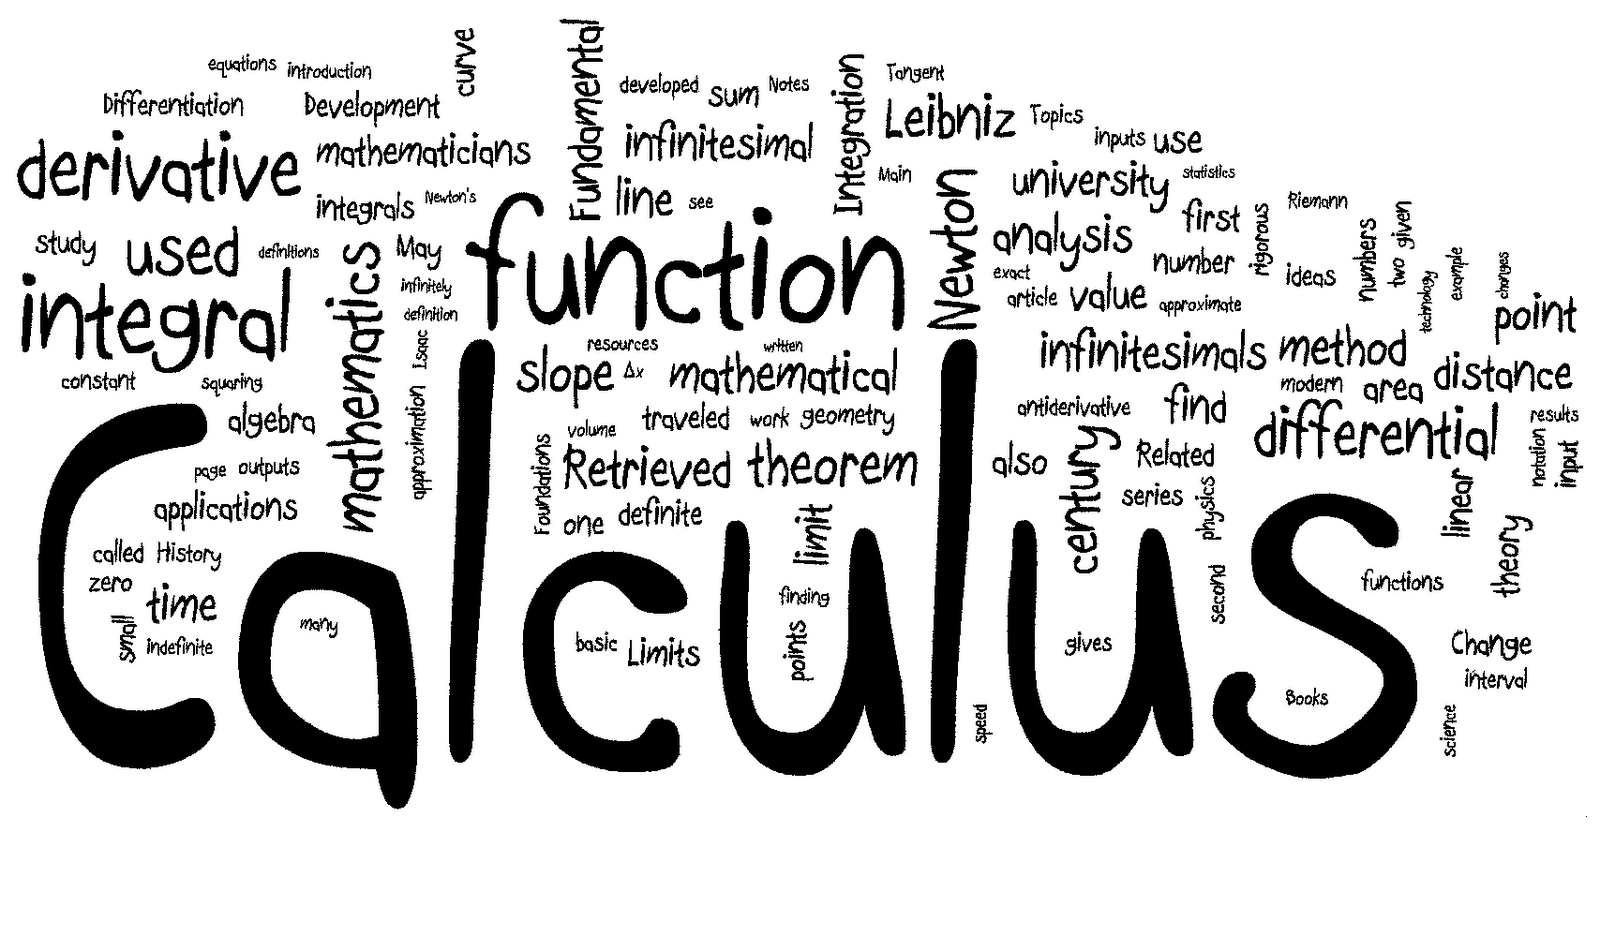
\includegraphics[width=0.98\textwidth]{calculus2.png}\\[1cm]
 \vfill
 
 
% Bottom of the page
{\large \today}
 
\end{center}
 
\end{titlepage}

\tableofcontents
\begin{abstract}
\begin{center}
	\small{\parbox{20cm}{
		\begin{raggedright}
		{\small
		\textit{Everybody is a genius. But if you judge a fish by its ability to climb a tree, it will live its whole life believing that it is stupid.}
 }
 
				\vspace{.5cm}\hfill{---Albert Einstein}
		\end{raggedright}
	}
} 
\end{center}
Calculus is one of the milestones of Western thought. Building on ideas of
Archimedes, Fermat, Newton, Leibniz, Cauchy, and many others, the calculus is
arguably the cornerstone of modern science. Any well-educated person should
at least be acquainted with the ideas of calculus, and a scientifically literate person
must know calculus solidly. Calculus has two main aspects: differential calculus and integral calculus.
Differential calculus concerns itself with rates of change. Various types of change,
both mathematical and physical, are described by a mathematical quantity called
the derivative. Integral calculus is concerned with a generalized type of addition,
or amalgamation, of quantities. Many kinds of summation, both mathematical and
physical, are described by a mathematical quantity called the integral.

\noindent Calculus is one of the most important parts of mathematics. It is fundamental to all
of modern science. How could one part of mathematics be of such central importance?
It is because calculus gives us the tools to study rates of change and motion.
All analytical subjects, from biology to physics to chemistry to engineering to mathematics,
involve studying quantities that are growing or shrinking or moving, in
other words, they are changing. Astronomers study the motions of the planets,
chemists study the interaction of substances, physicists study the interactions of
physical objects. All of these involve change and motion.
\footnote{To Archimedes, Pierre de Fermat, Isaac Newton, and Gottfried Wilhelm
von Leibniz, the fathers of calculus}
\footnote{The true sign of intelligence is not knowledge but imagination------
Albert Einstein }
\end{abstract}
\chapter{The Basics}
\begin{center}
	\small{\parbox{20cm}{
		\begin{raggedright}
		{\small
		\textit{Learning never exhausts the mind.}
 }
 
				\vspace{.5cm}\hfill{---Leonardo da Vinci}
		\end{raggedright}
	}
} 
\end{center}
\section{Number Systems}
Mathematics has its own language with numbers as the alphabet. The language is given structure
with the aid of connective symbols, rules of operation, and a rigorous mode of thought (logic). The number systems that we use in calculus are the \textit{natural numbers}, the \textit{integers}, the \textit{rational numbers}, and the \textit{real numbers}. Let us describe each of these :
\begin{enumerate}
\item  The \textbf{natural numbers} are the system of positive counting numbers $1,2,3\dots .$ We denote the set of all natural numbers by $\mathbb{N}$.
\[\mathbb{N}=\{1,2,3,4,5,6,7,8,\dots\}.\]
\item The \textbf{integers} are the positive and negative whole numbers and zero, $\dots ,-3,-2,-1,0,1,2,3,\dots .$ We denote the set of all integers by $\mathbb{Z}$.
\[\mathbb{Z}=\{\dots, -4,-3,-2,-1,0,1,2,3,4,\dots\}.\]
\item The \textbf{rational numbers} are quotients of integers or \textbf{fractions}, such as $\frac{2}{3}, -\frac{5}{4}$. Any number of the form $\dfrac{p}{q}$, with $p,q \in \mathbb{Z}$ and $q\neq 0$, is a rational number. We denote the set of all rational numbers by $\mathbb{Q}$.
\[\mathbb{Q}=\left\{\dfrac{p}{q}\biggl|p,q\in \mathbb{Z}, q\neq 0\right\}.\]
\item The \textbf{real numbers} are the set of all decimals, both terminating and non-terminating. We denote the set of all real numbers by $\mathbb{R}$. A decimal number of the form $x=3.16792$ is actually a rational number, for it represents 
\begin{equation*}
x=3.16792=\dfrac{316792}{100000}.
\end{equation*}
A decimal number of the form 
\begin{equation*}
m=4.27519191919\dots ,
\end{equation*}
with a group of digits that repeats itself interminably, is also a rational number.
To see this, notice that 
\begin{equation*}
100\cdot m=427.519191919\dots 
\end{equation*}  
and therefore we may subtract
\begin{eqnarray*}
100m=427.519191919\dots \\
m=4.27519191919\dots
\end{eqnarray*}
Subtracting, we see that 
\begin{equation*}
99m=423.244
\end{equation*}
or 
\begin{equation*}
m=\dfrac{423244}{99000}.
\end{equation*}
So, as we asserted, $m$ is a rational number  or quotient of integers. To  indicate recurring decimals we sometimes place dots over the repeating cycle of digits, e.g., $m=4.275\dot{1}\dot{9},\\ \frac{19}{6}=3.1\dot{6}$.

Another kind of decimal number is one which has a non-terminating decimal expansion \textit{that does not keep repeating}. An example is $\pi=3.14159265\dots $. Such a number is \textit{irrational}, that is, it \textit{cannot} be expressed as the quotient of two integers. 

In summary : There are three types of real numbers : (i)\, terminating decimals, \quad (ii)\, non-terminating decimals that repeat, \quad (iii)\, non-terminating decimals that do not repeat. Types (i) and (ii) are rational numbers. Type (iii) are irrational numbers.
 
The geometric representation of real numbers as points on a line is called the \textit{real axis}. Between any two rational numbers on the line there are infinitely many rational numbers. This leads us to call the set of rational numbers an \textit{everywhere dense set}.

Real numbers are characterised by three fundamental \textit{properties} :\\
\begin{enumerate}
\item \textbf{algebraic} means formalisations of the rules of calculation (addition, subtraction, multiplication, division). Example : $2(3+5)=2\cdot3 +2\cdot 5=6+10=16 $.
\item \textbf{order} denote inequalities. Example : $-\dfrac{3}{4}<\dfrac{1}{3}$.
\item \textbf{completeness} implies that there are ``no gaps'' on the real line.
\end{enumerate}
\textbf{Algebraic properties} of the reals for \textit{addition} ($a,b,c\in \mathbb{R}$) are :
\begin{itemize}
\item[(A1)] $a+(b+c)=(a+b)+c$. \textit{associativity}
\item[(A2)] $a+b=b+a$. \textit{commutativity}
\item[(A3)] There is a $0$ such that $a+0=a$.\quad  \textit{identity}
\item[(A4)] There is an $x$ such that $a+x=0$. \quad \textit{inverse}
\end{itemize}
Why these rules? They define an \textit{algebraic structure} (commutative group). Now define analogous algebraic properties for \textit{multiplication} :
\begin{itemize}
\item[(M1)] $a(bc)=(ab)c$.
\item[(M2)] $ab=ba$.
\item[(M3)] There is a $1$ such that $a\cdot 1=a$.
\item[(M4)] There is an $x$ such that $ax=1$ for $a\neq 0$.
\end{itemize}
Finally, connect \textit{multiplication} and \textit{addition} :
\begin{itemize}
\item[(D)] $a(b+c)=ab+ac$. \textit{distributivity}
\end{itemize}
These $9$ rules define an algebraic structure called a \textit{field}.

\textbf{Order properties} of the reals are :
\begin{itemize}
\item[(O1)] for any $a,b\in \mathbb{R}, \, a\leq b$ or $b\leq a$. \textit{totality of ordering I}
\item[(O2)] if $a\leq b$ and $b\leq a$, then $a=b$. \textit{totality of ordering II}
\item[(O3)] if $a\leq b$ and $b\leq c$, then $a\leq c$. \textit{transitivity}
\item[(O4)] if $a\leq b$, then $a+c\leq b+c$. \textit{order under addition}
\item[(O5)] if $a\leq b$ and $c\geq 0$, then $ac\leq bc$. \textit{order under multiplication} 
\end{itemize}
Some useful rules for calculations with inequalities are : If $a,b,c$ are real numbers, then :
\begin{enumerate}
\item if $a<b$ and $c<0 \Rightarrow bc<ac$.
\item if $a<b \Rightarrow -b<-a$.
\item if $a>0\Rightarrow \dfrac{1}{a}>0$.
\item if $a$ and $b$ are both positive or negative, then $a<b\Rightarrow \dfrac{1}{b} <\dfrac{1}{a}$.
\end{enumerate}
The \textbf{completeness property} can be understood by the following construction of the real numbers :
Start with the counting numbers $1,2,3,\dots .$
\begin{itemize}
\item $\mathbb{N}=\{1,2,3,4,\dots \}$ natural numbers $\Rightarrow$ Can we solve $a+x=b$ for $x$?
\item $\mathbb{Z}=\{\dots , -2,-1,0,1,2,\dots\}$ integers $\Rightarrow$ Can we solve  $ax=b$ for $x$?
\item $\mathbb{Q} =\{\frac{p}{q} | p,q \in \mathbb{Z}, q\neq 0\}$ rational numbers $\Rightarrow$ Can we solve $x^2=2$ for $x$?
\item $\mathbb{R}$ real numbers, for example : The positive solution to the equation $x^2=2$ is $\sqrt{2}$. This is an irrational number whose decimal representation is not eventually repeating.
\end{itemize}

\begin{equation*}
\Rightarrow \boxed {\mathbb{N}\subset \mathbb{Z}\subset \mathbb{Q}\subset \mathbb{R}}
\end{equation*}
In summary, the real numbers $\mathbb{R}$ are \textit{complete} in the sense that they correspond to all points on the real line, i.e., there are no ``holes'' or ``gaps'', whereas the rationals have ``holes'' (namely the irrationals).

\textbf{You Try It :} What type of real number is $3.41287548754875\dots$? Can you express this number in more compact form?
\end{enumerate}
\section{Intervals}
\begin{definition}
A subset of the real line is called an interval if it contains at least two numbers and all the real numbers between any of its elements.
\end{definition}
\textbf{Examples :} 
\begin{enumerate}
\item $x>-2$ defines an \textit{infinite interval}. Geometrically, it corresponds to a \textit{ray} on the real line.
\item $3\leq x\leq 6$ defines a \textit{finite interval}. Geometrically, it corresponds to a \textit{line segment} on the real line.
\end{enumerate}
\textbf{Finite Intervals.} Let $a$ and $b$ be two points such that $a<b$. By the \textit{open interval} $(a,b)$ we mean the set of all points between $a$ and $b$, that is, the set of all $x$ such that $a<x<b$. By the \textit{closed interval} $[a,b]$ we mean the set of all points between $a$ and $b$ or equal to $a$ or $b$, that is, the set of all $x$ such that $a\leq x\leq b$. The points $a$ and $b$ are called the \textit{endpoints} of the intervals $(a,b)$ and $[a,b]$.
\begin{center}
 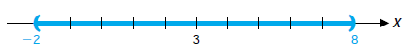
\includegraphics[width=0.4\textwidth]{open.png}\\[1cm]
  \end{center}
\noindent By a \textit{half-open interval} we mean an open interval $(a,b)$ together with one of its endpoints. There are two such intervals : $[a,b)$ is the set of all $x$ such that $a\leq x<b$ and $(a,b]$ is the set of all $x$ such that $a<x\leq b$.

\noindent \textbf{Infinite Intervals.} Let $a$ be any number. The set of all points $x$ such that $a<x$ is denoted by $(a,\infty)$, the set of all points $x$ such that $a\leq x$ is denoted by $[a,\infty)$. Similarly, $(-\infty ,b )$ denotes the set of all points $x$ such that $x<b$ and $(-\infty ,b]$ denotes the set of all $x$ such that $x\leq b$.
\begin{center}
 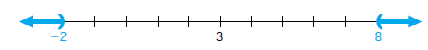
\includegraphics[width=0.4\textwidth]{infinite.png}\\[1cm]
  \end{center}
\section{Solving Inequalities}
Solve inequalities to find intervals of $x\in \mathbb{R}$. Set of all solutions is the \textit{solution set} of the inequality.
\textbf{Examples:}
\begin{enumerate}
\item \begin{eqnarray*}
2x-1 &<& x+3 \\
2x &<& x+4\\
x &<& 4.
\end{eqnarray*}
\item For what values of $x$ is $x+3(2-x)\geq 4-x$?
\begin{eqnarray*}
x+3(2-x) &\geq &  4-x \quad \hbox{when} \\
x+6-3x &\geq &  4-x\\
6-2x &\geq &  4-x\\
2 &\geq & x \Rightarrow x\leq 2.
\end{eqnarray*}
\item For what values of $x$ is $(x-4)(x+3)<0$?

\noindent \textbf{Case 1:}  \quad  $(x-4)>0$ \quad \hbox{and} \quad $(x+3)<0, \Longrightarrow x>4$ \quad \hbox{and}\quad $x<-3$. \\
\noindent \textbf{Impossible} \quad \hbox{since $x$ cannot be both greater than $4$ and less than $-3$}.\\
\noindent \textbf{Case 2:}  \quad $(x-4)<0$ \quad \hbox{and} \quad $(x+3)>0, \Longrightarrow x<4$ \quad \hbox{and} \quad $x>-3\Longrightarrow -3<x<4$.

\end{enumerate}
\textbf{You Try It:} Solve the inequality $\dfrac{2}{x-1}<\dfrac{3}{2x+1}$.
\section{The Absolute Value}
It is a quantity that gives the \textit{magnitude} or \textit{size} of a real number. The \textbf{absolute value} or \textbf{modulus} of a real number $x$, denoted by $|x|$, is given by 
\[|x| = \left\{ 
\begin{array}{l l}
  x, & \quad \hbox{if}~~~ x\geq 0 \\
 -x, & \quad \hbox{if}~~~ x<0.\\ \end{array} \right. \]
 Geometrically, $|x|$ is the distance between $x$ and $0$.  For example, $|-6|=6, \, |5|=5, \, |0|=0$.
 \begin{center}
 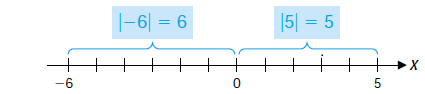
\includegraphics[width=0.4\textwidth]{absolute.png}\\[1cm]
  \end{center}
 \subsection{Properties of the Absolute Value }
 \begin{enumerate}
 \item The absolute value of a real number $x$ is non-negative, that is, $|x|\geq 0$.
 \item The absolute value of a real number $x$ is zero if and only if $x=0$, that is, $|x|=0\Longleftrightarrow x=0$.
 \item In general, if $x$ and $y$ are any two numbers, then 
 \begin{enumerate}
 \item $-|x|\leq x\leq |x|$.
 \item $|-x|=|x|$ and $|x-y|=|y-x|$.
 \item $|x|=|y|$ implies $x=\pm y$.
 \item $|xy|=|x|\cdot |y|$ and $\left|\dfrac{x}{y}\right|=\dfrac{|x|}{|y|}$ if $y\neq 0$.
 \item $|x+y|\leq |x|+|y|$. (Triangle inequality)
 \end{enumerate}
 \item If $a$ is any positive number, then 
 \begin{enumerate}
 \item $|x|=a$ if and only if $x=\pm a$.
 \item $|x|<a$ if and only if $-a<x<a$.
 \item $|x|>a$ if and only if $x>a$ or $x<-a$.
 \item $|x|\leq a$ if and only if $-a\leq x\leq a$.
 \item $|x|\geq a$ if and only if $x\geq a$ or $x\leq -a$.
 \end{enumerate}
 \end{enumerate}
 \textbf{Example:} Show that for all real numbers $x$, $|-x|=|x|$.\\
 \textbf{Solution:} If $x\in \mathbb{R}$, then either $x>0, x=0$ or $x<0$. If $x>0$, then $-x<0$. Thus, $|-x|=-(-x)=x=|x|$, that is, $|-x|=|x|$. \\
If $x=0$, then $|-x|=|-0|=|0|=0$, that is, $|-x|=|x|$.\\
If $x<0$, then $-x>0$. Now $|x|=-x=|-x|$ since $-x>0$.\\
Therefore in all cases $|-x|=|x|$.

\noindent \textbf{Solving an Equation with Absolute Values:} Solve the equation $|2x-3|=7$.

\noindent \textbf{Solution:} Hence $2x-3=\pm 7$, so there are two possibilities, 
\begin{eqnarray*}
2x-3 &=& 7 \quad  \quad 2x-3 =-7\\
2x &=& 10 \quad \quad 2x = -4\\
x &=& 5 \quad \quad x = -2
\end{eqnarray*}
The solutions of $|2x-3|=7$ are $x=5$ and $x=-2$.

\noindent \textbf{Solving Inequalities Involving Absolute values:} Sole the inequality $\left |5-\dfrac{2}{x}\right |<1$.

\textbf{Solution:} We have  
\begin{eqnarray*}
\left |5-\dfrac{2}{x}\right |<1 & \Longleftrightarrow &  -1<5-\dfrac{2}{x}<1\\
& \Longleftrightarrow & -6<-\dfrac{2}{x}<-4\\
 & \Longleftrightarrow & 3>\dfrac{1}{x}> 2\\
& \Longleftrightarrow  & \dfrac{1}{3}<x<\dfrac{1}{2}.
\end{eqnarray*}
Solve the inequalities and show the solution set on the real line. (a)\, $|2x-3|\leq 1$ \quad (b)\, $|2x-3|\geq 1$.

\noindent \textbf{Solution:} (a)\begin{eqnarray*}
|2x-3|\leq 1  & \Longleftrightarrow & -1\leq 2x-3 \leq 1\\
& \Longleftrightarrow &  2\leq 2x\leq 4\\
 &\Longleftrightarrow & 1\leq x\leq 2.
\end{eqnarray*}
The solution set is the closed interval $[1,2]$.

\noindent (b)\begin{eqnarray*}
|2x-3|\geq 1\Longleftrightarrow 2x-3\geq 1 \quad \hbox{or} \quad 2x-3 \leq -1 \\
\Longleftrightarrow x \geq 2 \quad \hbox{or} \quad x\leq 1.
\end{eqnarray*}
The solution set is $(-\infty , 1]\cup [2, \infty )$.

\noindent \textbf{You Try It:} Solve the inequality $4|x|<7x-6$.
\section{The Principle of Mathematical Induction}
It is an important property of the positive integers (natural numbers) and is used in proving statements involving all positive integers when it is known for, for example, that the statements are valid for $n=1,2,3,\dots $ but it is \textit{suspected} or \textit{conjectured} that they hold for all positive integers.
\subsection{Steps}
\begin{enumerate}
\item Prove the statement for $n=1$ or some other positive integer. (Initial Step)
\item Assume the statement true for $n=k$, where $k\in \mathbb{Z}^+$. (Inductive Hypothesis)
\item From the assumption in $2$ prove the statement must be true for $n=k+1$.
\item Since the statement is true for $n=1$ (from $1$) it must (from $3$) be true for $n=1+1=2$ and from this for $n=2+1=3$, and so on, so must be true for all positive integers. (Conclusion)
\end{enumerate}
\textbf{Example:} For any positive integer $n$, 
\[1+2+\cdots + n=\dfrac{n(n+1)}{2}.\]
\textbf{Solution:} \begin{enumerate}
\item Prove for $n=1$, $1=\dfrac{1(1+1)}{2}=\dfrac{2}{2}=1$, which is clearly true.
\item Assume that the statement holds for $n=k$, that is, 
\[1+2+\cdots +k =\dfrac{k(k+1)}{2}.\]
\item Prove for $n=k+1$. So 
\begin{eqnarray*}
1+2+\cdots + k+(k+1) &=& \dfrac{k(k+1)}{2}+(k+1)\quad \hbox{(by inductive hypothesis)}\\
&=& \dfrac{k(k+1)+2(k+1)}{2}\\
&=& \dfrac{k^2+3k+2}{2}\\
&=& \dfrac{(k+1)(k+2)}{2}
\end{eqnarray*}
so holds for $n=k+1$.
\item Hence by induction, $1+2+\cdots +n=\dfrac{n(n+1)}{2}$ is true for any positive integer $n$.
\end{enumerate}
\textbf{Example:} Prove that for any natural number 
\begin{equation*}
1+3+5+\cdots + 2n-1=n^2.
\end{equation*}
\textbf{Solution:} \begin{enumerate}
\item Prove for $n=1$, $1=1^2=1$, so it is true.
\item Assume that the statement holds for $n=k$, that is, 
\begin{equation*}
1+3+5+\cdots +2k-1=k^2.
\end{equation*} 
\item Prove for $n=k+1$. We have 
\begin{eqnarray*}
1+3+5+\cdots +(2k-1)+2(k+1)-1 &=& k^2+2k+1\quad \hbox{(by inductive hypothesis)}\\
&=& (k+1)^2.
\end{eqnarray*}
So it is true for $n=k+1$. 
\item Hence by induction  $1+3+5+\cdots + 2n-1=n^2$ is true for all natural numbers $n$.
\end{enumerate}
\newpage
\textbf{Example:} Prove that $3^n>2^n$ for all natural numbers $n$.\\

 \textbf{Solution:} 
\begin{enumerate}
\item Prove for $n=1 \Longrightarrow 3^1=3>2^1=2$, which is true.
\item Assume the statements holds for $n=k$, that is, $3^k>2^k$.
\item Prove for $n=k+1$. 
\begin{eqnarray*}
3^{k+1} &=& 3^k\cdot 3\\
&>& 2^k \cdot 3 \quad \hbox{by inductive hypothesis}\\
&>& 2^k\cdot 2 \quad \hbox{since $3>2$}\\
&>& 2^{k+1},
\end{eqnarray*}
which is true.
\item Hence, by induction $3^n>2^n$ for all natural numbers $n$.
\end{enumerate}
\textbf{Example:} Prove that for any integer $n\geq 1$, $2^{2n}-1$ is divisible by $3$.\\
\textbf{Solution:}
\begin{enumerate}
\item Prove for $n=1 \Longrightarrow 2^2-1=3$ and is divisible by $3$, hence its true.
\item Assume that the statement holds for $n=k$, that is, for $k\geq 1$, $2^{2k}-1$ is divisible by $3$, i.e., $2^{2k}-1=3l$, for some $l\in \mathbb{Z}$.
\item Prove for $n=k+1$.
\begin{eqnarray*}
2^{2(k+1)}-1 &=& 4\cdot 2^{2k} -1 \quad \hbox{but $2^{2k}=3l+1$ by the inductive hypothesis}\\
&=& 4(3l+1)-1\\
&=& 12l+4-1\\
&=& 12l+3\\
&=& 3(4l+1), 
\end{eqnarray*}
which is true.
\item Hence, by induction $2^{2n}-1$ is divisible by $3$ for all $n\geq 1$.
\end{enumerate}
\section{Tutorial Questions}
\begin{enumerate}
\item Find a rational number whose decimal expansion is $1.63636363\dots$.
\item Explain why $\pi \neq \frac{22}{7}$.
\item State, giving a reason, whether each of the following numbers is rational or irrational.\\
(i)\, $0.20200200020\dots$ \quad (ii)\, $537.137137137\dots$.
\item Show that $a^2+b^2 \geq 2ab$, for all $a,b \in \mathbb{R}$.
\item Show that if $a^2+b^2=1$ and $c^2+d^2=1$, then $ac+bd \leq 1$.
\item Show that if $0<a<b$ then $a^2<b^2$. If $a^2<b^2$, is it necessarily true that $a<b$? Give an example to illustrate your answer.
\item Solve the following inequalities.\\
(i)\, $|x+1| \geq 3$ \quad (ii)\, $\dfrac{2x+3}{x-5}>3$ \quad (iii)\, $2|x|>3x-10$ \quad (iv)\, $x^2+x-2>0$ \\ (v)\, $2|x|-1>3|x|-3$ \quad (vi)\, $4|x|<7x-6$ \quad (vii)\, $\dfrac{|x|+2}{x-2}<4$ \quad (viii)\, $|x-4|=9$. 
\item Prove that $|ab|=|a||b|$ for all $a,b \in \mathbb{R}$.
\item Show that $|a+b|\leq |a|+|b|$ for all $a,b \in \mathbb{R}$.
\item Prove that $|x|^2=x^2$ for any real number $x$.
\item If $x$ and $y$ are real numbers, prove that $|x|-|y|\leq |x-y|$.
\item Prove the following by induction.
\begin{itemize}
\item[(a)] $n! >2^n$ for all $n \geq 4$.
\item[(b)] For all $n\geq 1$ and $f(x)=x^n$, then $f'(x)=nx^{n-1}$.
\item[(c)] $n^2 \leq 2^n$ for all $n \geq 5$.
\item[(d)] The sum of terms in a geometric series is $\displaystyle \sum _{i=0}^{n}{r^i}=\dfrac{r^{n+1}-1}{r-1}$, if $r \neq 0, r \neq 1, n\in \mathbb{N}$.
\item[(e)] $1+2+ \cdots +n =\dfrac{n(n+1)}{2}$.
\item[(f)] For any positive integer $n$, $n^3+2n$ is divisible by $3$.
\item[(g)] $3^n>n^2$ for $n>2$.
\item[(h)] $7^{2n}-48n-1$ is divisible by $2304$.
\item[(i)] All numbers of the form $8^n-2^n$ are divisible by $6$.
\item[(j)] $11^n-4^n$ is divisible by $7$ for all $n \in \mathbb{Z ^+}$.
\item[(k)] $|\sin nx| \leq n|\sin x|$ for all $x \in \mathbb{R}, n \in \mathbb{Z ^+}$.
\item[(l)] $1^3+2^3+3^3+\cdots +n^3=\dfrac{n^2(n+1)^2}{4}$.
\item[(m)] Prove \textit{Bernoulli's inequality}, $(1+x)^n>1+nx$, for $n=2,3,\dots$, if $x>-1, \, x\neq 0$.
\item[(n)] $1^2+2^2+3^2+\cdots +n^2=\dfrac{1}{6}n(n+1)(2n+1)$.
\item[(o)] Prove that if $a_1, a_2, a_3, \dots , a_n$ are real numbers, then 
\begin{equation*}
|a_1+a_2+\cdots +a_n|\leq |a_1| +|a_2|+\cdots +|a_n|.
\end{equation*}
\item[(p)] Prove that, if $\sin x \neq 0$ and $n$ is a natural number, then 
\begin{equation*}
\cos x \cdot \cos 2x \cdot \cdots \cos 2^{n-1} x =\dfrac{\sin 2^n x}{2^n\sin x}.
\end{equation*} 
\end{itemize}
\end{enumerate}
\chapter{Functions}
\begin{center}
	\small{\parbox{18cm}{
		\begin{raggedright}
		{\small
		\textit{We know that God exists because Mathematics is consistent and we know that the devil exists because we cannot prove the consistency.}
 }
 
				\vspace{.5cm}\hfill{---Andre Weil}
		\end{raggedright}
	}
} 
\end{center}
\section{What is a Function?}
\noindent A function is a \textit{rule} or a \textit{correspondence}, relating two sets in such a manner that each element in the first set corresponds to one and only one element in the second set. What do we mean when we say $\boxed{y ~~is~~ a ~~function~~ of~~ x?}$ Symbolically, we write $y=f(x)$, where 
\begin{enumerate}
\item $x$ is the \textit{independent variable}. (input value of $f$)
\item $y$ is the \textit{dependent variable}. (output value of $f$ at $x$)
\item $f$ is a \textit{function}. (rule that assigns $x$ to $y$)
\end{enumerate}
\begin{definition}
A function $f$ from a set $X$ to a set $Y$ is a rule that assigns to each element $x$ in $X$ a unique element $y$ in $Y$.
\end{definition}
The set $X$ is called the \textbf{domain} of $f$ and the set of corresponding elements $y$ in $Y$ is called the \textbf{range} of $f$ where sets $X$ and $Y$ consists of real numbers. We write $f :X\to Y$.

\noindent \textbf{Examples:} Stock market index depending on time, volume of sphere depending on radius, circle of a given radius has only one area.

\noindent Let $f$ be a function. The number $y$ in the range that corresponds to a selected number $x$ in the domain is said to be the value of the function at $x$, or \textbf{image} of $x$, written $f(x)$, so $y=f(x)$.

\noindent \textbf{Examples:} $f(x)=3x^4+2$, $g(t)=4-t^2$, $h(s)=2s^2+7$.

\noindent The \textbf{domain} of a function $f$ is the largest set of real numbers for which the rule makes sense.
\begin{center}
 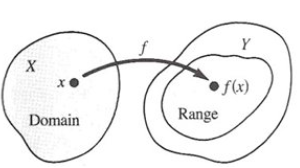
\includegraphics[width=0.4\textwidth]{function1.png}\\[1cm]
  \end{center}
 \textbf{Example:} Let $f(x)=\dfrac{1}{x}$, we cannot compute $f(0)$, since $\dfrac{1}{0}$ is not defined. Then the domain of $f(x)=\dfrac{1}{x}$ is the set of all real numbers except $0$.

\begin{table}[h]
\centering
\begin{tabular}{|l|c|c|}
\hline
\textbf{Function} & \textbf{Domain} $x\in X$ & \textbf{Range} $y\in Y$\\
\hline
$y=x^2$ & $(-\infty , \infty)$ & $[0,\infty)$ \\
$y=\dfrac{1}{x}$ & $(-\infty , 0)\cup (0, \infty)$ & $(-\infty , 0)\cup (0, \infty)$\\
$y=\sqrt{x}$ & $[0,\infty )$ &$[0,\infty )$\\
 $y=\sqrt{1-x^2}$ & $[-1,1]$ & $[0,1]$\\
\hline
\end{tabular}
\caption{Examples of functions}
\label{tab:template}
\end{table}

\noindent \textbf{You Try It:} Let 
\begin{equation*}
g(x)=\dfrac{x}{x^2+4x+3}.
\end{equation*}
What is the domain and range of this function?
\section{Graphs of Functions}
It is useful to draw pictures which represent functions. These pictures, or \textit{graphs}, are a device for helping us to think about functions. We graph functions in the $x-y$ pane. The elements of the domain of the function are thought of as points of the $x-$axis. The values of a function are measured on the $y-$axis.The graph of $f$ associates to $x$ a unique $y$ value that the function $f$ assigns to $x$. 
The \textbf{graph} of a function $f$ is the set of points $\{(x,y)| y=f(x) \quad \hbox{in the domain of $f$}\}$ in the Cartesian plane.

\noindent As a consequence, a function is characterised geometrically by the fact that any vertical line intersecting its graph does so in \textit{exactly one point}.
\begin{center}
 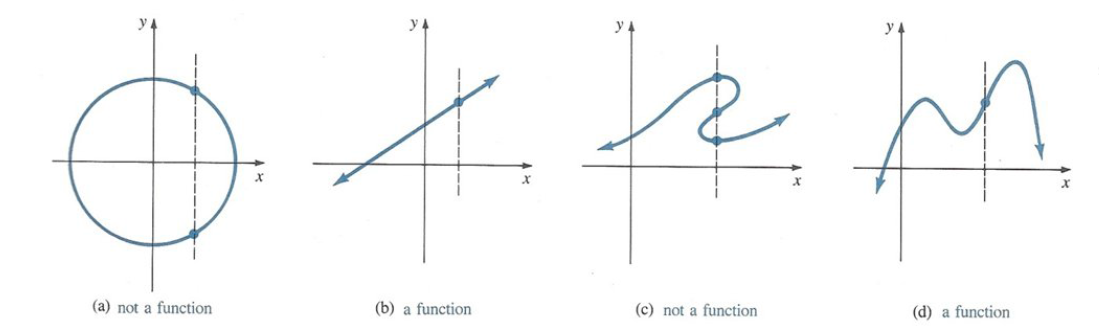
\includegraphics[width=0.89\textwidth]{2.png}\\[1cm]
  \end{center}

\section{Bounded Functions}
If there is a constant $M$ such that $f(x)\leq M$ for all $x$ in the interval (or other set of numbers), we say that $f$ is \textit{bounded above} in the interval (or the set) and call $M$ an \textit{upper bound} of the function. If a constant $m$ exists such that $f(x)\geq m$ for all $x$ in an interval, we sat that $f(x)$ is \textit{bounded below} in the interval and call $m$ a \textit{lower bound}. If $m\leq f(x)\leq M$ in an interval, we call $f(x)$ \textit{bounded}.

\noindent \textbf{Examples:} $f(x)=x+3$ is bounded in $-1\leq x\leq 1$. An upper bound is $4$ (or any number grater than $4$). A lower bound is $2$ (or any number less than $2$).  
\section{Types of Functions}
\subsection{Elementary Functions}
\subsubsection{Polynomial Function}
Have the form $f(x)=a_0x^n+a_1x^{n-1}+\cdots + a_{n-1}x+a_n$ where $a_0, a_1, \dots , a_n$ are constants and $n$ is a positive integer called the degree of the polynomial provided $a_0\neq 0$. 

\noindent \textbf{Examples:} $x^5+10x^3-2x+1$ is a polynomial of degree $5$.
\subsubsection{Rational Functions}
A function $f(x)=\dfrac{P(x)}{Q(x)}$ where $P(x)$ and $Q(x)$ are polynomial functions.

\noindent \textbf{Example:} $f(x)=\dfrac{x^3+x+5}{x^2-3x-4}$ is a rational function. Since $(x+1)(x-4)$ and $(x+1)(x-4)=0$ for $x=-1$ and $x=4$, the domain of $f$ is the set of all real numbers except $-1$ and $4$.  
\subsubsection{Power Function}
$f(x)=kx^n$, $n$ a real number and $k$ a constant. 
\begin{center}
 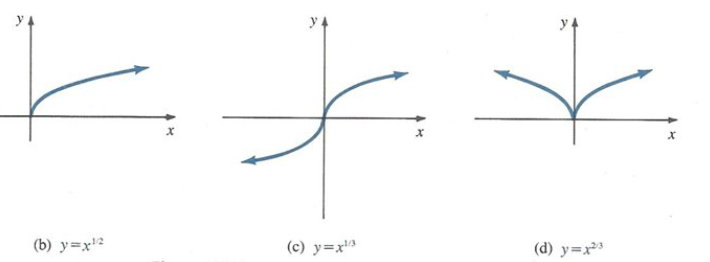
\includegraphics[width=0.6\textwidth]{power.png}\\[1cm]
  \end{center}
\noindent \textbf{Examples:} $y=\dfrac{1}{x}$, $y=x^{\frac{1}{2}}$, $y=x^{\frac{2}{3}}$.
\subsubsection{Piecewise Defined Functions}
A function need not be defined by a single formula. A piecewise defined function is a function described by using \textit{different formula on different parts of its domain}.

\noindent \textbf{Examples:} (a)\,  $f(x) = \left\{ 
\begin{array}{l l}
  -1, & \quad  x<0 \\
 0, & \quad x=0\\
 x+2, & \quad x>0\\ \end{array} \right. $ \quad (b)\, $f(x) = \left\{ 
\begin{array}{l l}
  -x, & \quad  x< 0 \\
 x^2, & \quad 0\leq x\leq 1\\
 1, & \quad x>1.\\ \end{array} \right. $
 \begin{center}
 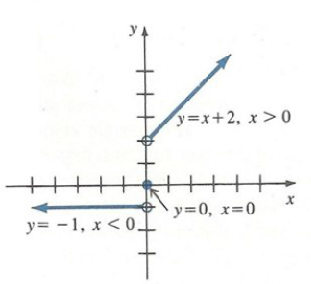
\includegraphics[width=0.6\textwidth]{piece.png}\\[1cm]
  \end{center}
 \subsubsection*{Transcendental  Functions}
 The following are sometimes called \textit{elementary transcendental functions}.
 \begin{enumerate}
 \item  Exponential function, $f(x)=a^x, a\neq 0,1$.
 \item Logarithmic  function, $f(x)=\log _a x, a\neq 0,1$.
 \item Trigonometric functions (also called circular functions because of their geometric interpretation with respect to the unit circle), e.g., $\sin x, \cos x, \tan x =\dfrac{\sin x}{\cos x}, \csc x, \cot x, \sec x$.
 \item Inverse trigonometric functions, e.g., $y=\sin ^{-1} x, y=\cos ^{-1} x$.
 \item Hyperbolic Functions, e.g., $\sinh x, \cosh x, \tanh x, \coth x$.
  \end{enumerate}
  \subsubsection{Even and Odd Functions}
  Let $f(x)$ be a \textit{real-valued} function of a real variable. Then $f$ is \textit{even} if $f(x)=f(-x)$. (Symmetric with respect to the $y-$axis)
  
\noindent \textbf{Examples:} $|x|, x^2, x^4, \cos x, \cosh x$.

\noindent Let $f(x)$ be a real-valued function of a real variable. Then $f$ is \textit{odd} if $-f(x)=f(-x)$ or \\$f(x)+f(-x)=0$. (Symmetric with respect to the origin)

\noindent \textbf{Examples:} $x, x^3, \sin x, \sinh x$.

\noindent \textbf{Example:} Determine whether the following function is odd or even $f(x)=\dfrac{3x}{x^2+1}$.

\noindent \textbf{Solution:} \begin{equation*}
f(-x)=\dfrac{3(-x)}{(-x)^2+1}=-\dfrac{3x}{x^2+1}=-f(x).
\end{equation*}
The function is odd.
\section{Combining Functions}
A function $f$ can be combined with another function $g$ by means of arithmetic operations to form other functions, the \textbf{sum} $f+g$, \textbf{difference} $f-g$, \textbf{product} $fg$ and \textbf{quotient} $\dfrac{f}{g}$ are defined as : Let $f$ and $g$ denote functions, then 
\begin{enumerate}
\item \underline{Sum} : $(f+g)(x)=f(x)+g(x)$.
\item \underline{Difference} : $(f-g)(x)=f(x)-g(x)$.
\item \underline{Product} : $(fg)(x)=f(x)g(x)$.
\item \underline{Quotient} : $\left(\dfrac{f}{g}\right )(x)=\dfrac{f(x)}{g(x)}$.
\end{enumerate}
\textbf{Example:} If $f(x)=2x^2-5$ and $g(x)=3x+4$. Find $f+g, f-g, fg, \dfrac{f}{g}$.

\noindent \textbf{Solution:} \begin{eqnarray*}
(f+g)(x) &=& (2x^2-5)+(3x+4)= 2x^2+3x-1.\\
(f-g)(x)&=& (2x^2-5)-(3x+4)= 2x^2-3x-9.\\
(fg)(x)&=&(2x^2-5)(3x+4) = 6x^3+8x^2-15x-20\\
\left(\dfrac{f}{g}\right)(x)&=& \dfrac{2x^2-5}{3x+4}.\\
\end{eqnarray*}
\section{Composition of Functions}
Let $f$ and $g$ denote functions. The \textbf{composition } of $f$ and $g$, written $f\circ g$ is the function $(f\circ g)(x)=f(g(x))$ and the composition of $g$ and $f$, written $g\circ f$, is the function $(g\circ f)(x)=g(f(x))$.

\noindent \textbf{Example:} If $f(x)=x^2$ and $g(x)=x^2+1$, find $f\circ g$ and $g \circ f$.

\noindent \textbf{Solution:} \begin{equation*}
(f\circ g)(x)=f(g(x))=f(x^2+1)=(x^2+1)^2=x^4+2x^2+1.
\end{equation*}
and \begin{equation*}
(g\circ f)(x)=g(f(x))=g(x^2)=(x^2)^2+1=x^4+1.
\end{equation*}
In general, $f\circ g \neq g\circ f$.
\section{Bijection, Injection and Surjection}
Classes of functions may be distinguished by the manner in which arguments and images are related or \textit{mapped} to each other.

\noindent A function $f:X\to Y$ is \textbf{injective (one-to-one, $1-1$)} if every element of the range corresponds to exactly one element in its domain $X$.

\noindent For all $x,y\in X$, $f(x)=f(y)\Longrightarrow x=y$ or equivalently

\noindent For all $x,y\in X$, $x\neq y\Longrightarrow f(x)\neq f(y)$.  An injective function is an \textbf{injection}.

\begin{center}
 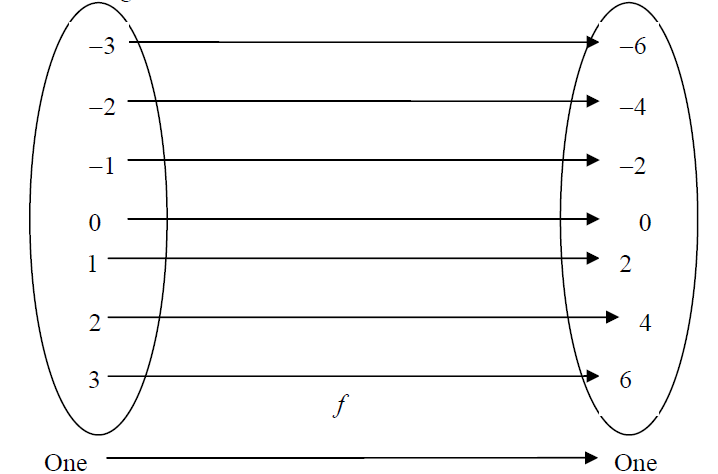
\includegraphics[width=0.6\textwidth]{one.png}\\[1cm]
  \end{center}
\noindent \textbf{Example:} Show that the functions $f(x)=2x+3$ and $g(x)=x^3-2$ are injective.

\noindent \textbf{Solution:} Need to show that $f(x)=f(y)\Longrightarrow x=y$.
\begin{eqnarray*}
2x+3 &=& 2y+3 \\
2x &=& 2y \Longrightarrow x =y.\\
\end{eqnarray*}
Hence $f(x)=2x+3$ is injective.

\noindent Need to show that $g(x)=g(y)\Longrightarrow x=y$.
\begin{eqnarray*}
x^3-2 &=& y^3-2 \\
x^3 &=& y^3 \quad  \hbox{taking cube roots}\\
x &=& y.
\end{eqnarray*}
Hence $g(x)=x^3-2$ is injective.

\noindent A function $f:X\to Y$ is called \textbf{onto} if for all $y$ in $Y$ there is an $x$ in $X$ such that $f(x)=y$. All elements in $Y$ are used. Such functions are referred to as \textbf{surjective}.
\begin{center}
 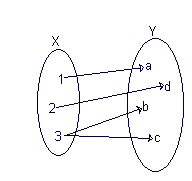
\includegraphics[width=0.2\textwidth]{save.png}\\[1cm]
  \end{center}
\noindent \textbf{Example:} Show that $f(x)=3x-5$ is onto.

\noindent \textbf{Solution:} For \textit{onto} $f(x)=y$, i.e., $3x-5=y$. Solve for $x$, $\Longrightarrow x=\dfrac{y+5}{3}$.\\ So $f\left (\dfrac{y+5}{3}\right)=3\left(\dfrac{y+5}{3} \right)-5=y$. Therefore $f$ is onto.

\noindent  Let $X$ and $Y$ be sets. A function $f:X\to Y$ that is one-to-one and onto is called a \textit{bijection} or \textit{bijective function from $X$ to $Y$}. If $f$ is both one-to-one and onto, then we call $f$ a $1-1$ correspondence.

\noindent \textbf{Inverse of a Function.} Suppose $f$ is a $1-1$ function that has domain $X$ and range $Y$. Since every element $y\in Y$ corresponds with precisely one element $x$ of $X$, the function $f$ must actually determine a \textit{reverse} function $g$ whose domain is $Y$ and range is $X$, where $f$ and $g$ must satisfy $f(x)=y$ and $g(y)=x$. The function $g$ is given the formal name \textit{inverse} of $f$ and usually written $f^{-1}$ and read $f$ inverse. Not all functions have inverses, those that do are called \textit{invertible functions}.
\begin{center}
 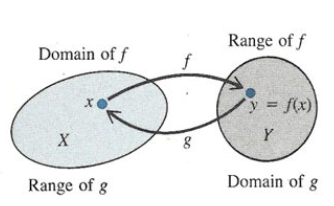
\includegraphics[width=0.6\textwidth]{inverse.png}\\[1cm]
  \end{center}
\noindent \textbf{Example:} Find the inverse of the function $f(x)=(2x+8)^3$.

\noindent \textbf{Solution:} We must solve the equation $y=(2x+8)^3$ for $x$.
\begin{eqnarray*}
y &=& (2x+8)^3\\
\sqrt[3]{y} &=& 2x+8 \\
\sqrt[3]{y}-8 &=& 2x \\
x &=& \dfrac{\sqrt[3]{y}-8}{2}.
\end{eqnarray*}
Hence the inverse function $f^{-1}$ is given by $f^{-1}(x)= \dfrac{\sqrt[3]{x}-8}{2}$.

\noindent A $1-1$ function $f$ can have only one inverse, i.e., $f^{-1}$ is unique. A function $f:X\to Y$ is \textbf{invertible} if and only if $f$ is one-to-one and maps $X$ onto $Y$.

\section{Operations on Functions}
\subsubsection{Equality of Functions}
Equality of functions does not mean the same as equality of two numbers (numbers have a fixed value but values of functions vary). Each function is a relationship between $x$ and $y$, the two relationships are the same if for every value of $x$ we get the same value of $y$.

\noindent \textbf{Example:} The functions $(x-1)(x+2)$ and $x^2+x-2$ are equal.

\noindent \textbf{Example:} Equal functions for positive values of $x$,
\begin{equation*}
|x| =\sqrt{x^2}.
\end{equation*}
\subsubsection{Identity Function}
Generally, an identity function is one which does not change the domain values at all. Its the function $f(x)=x$. Denoted by $I_X$.
\begin{center}
 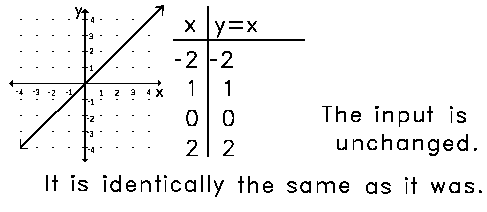
\includegraphics[width=0.6\textwidth]{identity.png}\\[1cm]
  \end{center}
\subsubsection{Monotonic Functions}
A function is called \textit{monotonic increasing} in an interval, if for any two points $x_1$ and $x_2$ in the interval such that if $x_1<x_2, \, f(x_1)\leq f(x_2)$. If $f(x_1)<f(x_2)$ the function is called \textit{strictly increasing}.

\noindent \textbf{Similarly}, if $f(x_1)\geq f(x_2)$ whenever $x_1< x_2$, then $f(x)$ is \textit{monotonic decreasing},  while if \\$f(x_1)>f(x_2)$ it is \textit{strictly decreasing}.
\section{Tutorial Questions}
\begin{enumerate}
\item Find the domain of each of the following functions.\\
(i)\, $-\sqrt{9-x^2}$  \quad (ii)\, $\dfrac{1}{\sqrt{1-x}}$ \quad (iii)\, $\dfrac{1}{2x+3}$ \quad (iv)\, $\sqrt{(3-x)(2x+4)}$ \quad (v)\, $\dfrac{x-2}{x^2-4}$ \\ (vi)\, $\ln (x^3-3x^2-4x+12)$ \quad (vii)\, $\dfrac{x^3-8}{x^2-4}$ \quad (viii)\, $\sqrt{\sin 5x}$ \quad  (ix)\, $\ln (2x^2-5x-12)$ \\(x)\, $\dfrac{1}{\sqrt{9-x^2}}$ \quad (xi)\, $\sqrt{x^2-4}$ \quad (xii)\, $x^2+4$ \quad (xiii)\, $\sqrt{\dfrac{x}{2-x}}$.
\item If $f(x)=\dfrac{x-1}{x+1}$, find (i)\, $f(0)$ \quad (ii)\, $f(1)$ \quad (iii)\, $f(-2)$. Show that $f\left(\dfrac{1}{x}\right)=-f(x)$ and $f\left(-\dfrac{1}{x}\right)=-\dfrac{1}{f(x)}$.
\item If $f(x)=\dfrac{1}{x}$, show that $f(a)-f(b)=f\left(\dfrac{ab}{b-a} \right)$.
\item If $f(x)=x^2-x$, show that $f(x+1)=f(-x)$.
\item If $y=f(x)=\dfrac{5x+3}{4x-5}$, show that $x=f(y)$.
\item Determine whether or not each of the following correspondences is a function.\\
(i)\, $x^2+y=1$ \quad (ii)\, $x^2y^2=5$ \quad (iii)\, $x^2y=4$ \quad (iv)\, $\{(1,5), (2,5), (5,1)\}$.
\item For each of the following pairs of functions, calculate $f\circ g$ and $g\circ f$.
\begin{itemize}
\item[(i)] $f(x)=\sin (x+3x^2)$ and $g(x)=\cos (x^2-x)$.
\item[(ii)] $f(x)=e^{x^2}$ and $g(x)=e^{-x^2}$.
\item[(iii)] $f(x)=x(x+1)(x+2)$ and $g(x)=(2x-3)(x+4)$.
\end{itemize}
\item Determine whether each of the pairs of the following functions are equal and if they are not equal, give where they are equal.\\
(i)\, $f(x)=\sqrt{x^2}, \quad g(x)=(\sqrt{x})^2$ \quad (ii)\, $f(x)=x^2, \quad g(x)=x|x|$.
\item Show that if $ad-bc\neq 0$, then the function $f(x)=\dfrac{ax+b}{cx+d}$ is one-to-one and find its inverse, stating the domains of both the function and its inverse. What happens if $ad-bc=0$?
\item Show that these functions are a one-to-one correspondence. Find their inverses.\\
(i)\, $f(x)=2x+3$ \quad (ii)\, $g(x)=x^3-2$ \quad (iii)\, $h(x)=(x-2)^2$ \quad (iv)\, $k(x)=\sqrt[3]{x}+7$.
\item Show that the function $f(x)=\ln (x+\sqrt{x^2+1})$ is an odd function and find the inverse function of $f(x)$.
\end{enumerate}
\chapter{Sequences}
\begin{center}
	\small{\parbox{18cm}{
		\begin{raggedright}
		{\small
		\textit{A girl and a boy jump into a river. The boy swims over to the girl and says, ``God, it's cold." What's the probability they will kiss?}
 }
 
				\vspace{.5cm}\hfill{---Jenny Downham, You Against Me }
		\end{raggedright}
	}
} 
\end{center}
\begin{definition}
A \textbf{sequence} is a set of numbers $u_1, u_2, u_3, \dots$ in a definite order of arrangement and formed according to a definite rule.
\end{definition}
\noindent Each number in the sequence is called a \textit{term} and $u_n$ is called the \textit{$n$th term}. The sequence $u_1,u_2,u_3, \dots$ is written briefly as  $\{u_n\}$, e.g., $\{u_n\}=2n$, where $u_1=2$, $u_2=4$, $u_3=6$ and so on. A sequence can be \textit{finite} or \textit{infinite}. A finite sequence has only definite number of terms. An infinite sequence is non-terminating, e.g., $u_n=\dfrac{1}{2n-1}$.

\noindent \textbf{Recursive Definitions.} The values of the terms in a sequence may be given explicitly by formulas such as $u_n=n^3-73n$. 

\noindent A \textbf{recursive calculation} finds the value of $u_n$ by looking to see which terms $u_n$ depends on, then which terms depend, and so on.

\noindent \textbf{Example:} $u_0=1, \quad u_{n+1}=\dfrac{2}{u_n}, \quad n\in \mathbb{N}$.

\noindent \textbf{Solution:} 
\begin{eqnarray*}
u_1 &=& u_{0+1} = \dfrac{2}{u_0}=\dfrac{2}{1}=2\\
u_2 &=& u_{1+1}= \dfrac{2}{u_1} =\dfrac{2}{2}=1\\
u_3 &=& u_{2+1} = \dfrac{2}{u_2} =\dfrac{2}{1}=2.
\end{eqnarray*} 
\textbf{You Try It:} Define recursively 
\begin{equation*}
a_0=a_1=1, \quad \hbox{and} \quad a_n=a_{n-1}+2a_{n-2}, \, n\geq 2.
\end{equation*}
Find $a_6$ recursively.
\section{Limits of Sequences}
Lets consider the sequence $u_n=\dfrac{1}{n}$. The sequence has the terms $1, \frac{1}{2}, \frac{1}{3}, \frac{1}{4}, \dots$. We see that the terms of the sequence \textit{tend to} or \textit{approach} $0$.

\begin{definition}
A number $L$ is called the \textbf{limit} of an infinite sequence $a_1, a_2,a_3, \dots$ or $\{a_n\}$, if for any positive number $\varepsilon$, we can find a positive number $N$ depending on $\varepsilon$ such that $|a_n-L|<\varepsilon$ for all integers $n>N$. We write $\displaystyle \lim _{n\rightarrow \infty} a_n=L$.
\end{definition}
\noindent If $\{a_n\}$ is a convergent sequence, it means that the terms $a_n$ can be made arbitrarily close to $L$ for $n$ sufficiently large.
\begin{center}
 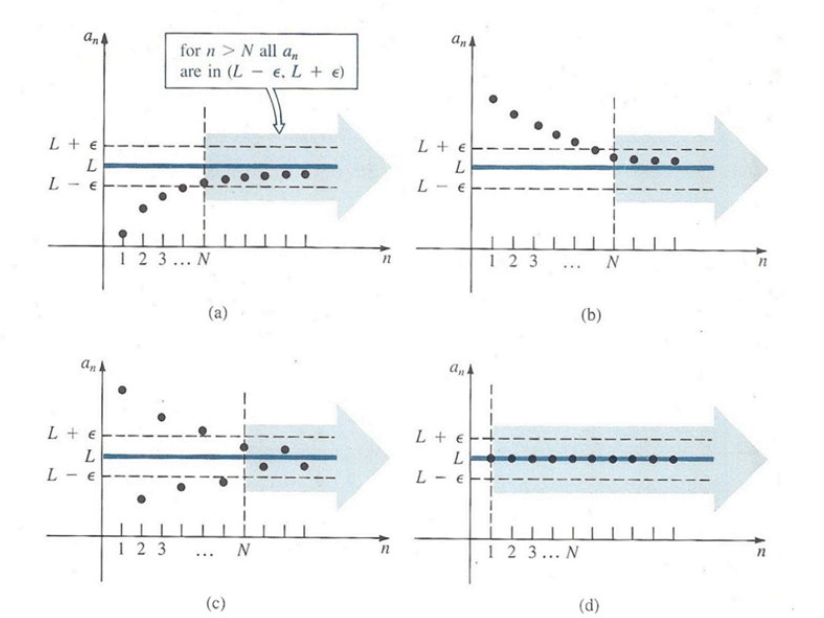
\includegraphics[width=0.7\textwidth]{seq.png}\\[1cm]
  \end{center}
\noindent \textbf{Example:} If $u_n=3+\dfrac{1}{n}=\dfrac{3n+1}{n}$, the sequence is $4, \frac{7}{2}, \frac{10}{3}, \dots$and we can show that \\ $\displaystyle \lim _{n\rightarrow \infty} u_n=3$.

\noindent If the limit of a sequence exists, the sequence is called \textbf{convergent}, otherwise, it is called \textbf{divergent}.

\noindent \textbf{Example:} Prove that $\displaystyle \lim _{n\rightarrow \infty} \frac{1}{n}=0$.

\noindent \textbf{Proof:} Let $\varepsilon >0$, we can find $N(\varepsilon)$ such that $\left|\dfrac{1}{n}-0\right|=\left|\dfrac{1}{n}\right|=\dfrac{1}{n} <\varepsilon$.  But $n>\dfrac{1}{\varepsilon}$. So $N=\dfrac{1}{\varepsilon}$. Taking $N$ to be the smallest integer greater than $ \dfrac{1}{\varepsilon}$, we have, $\displaystyle \lim _{n\rightarrow \infty} \dfrac{1}{n}=0$.

\noindent \textbf{You Try It:} Prove that $\displaystyle \lim _{n\rightarrow 0} \dfrac{1}{n^p}=0$ if $p\in \mathbb{N}$.

\noindent \textbf{Example:} Use the definition of a limit to prove that $\displaystyle \lim _{n\rightarrow \infty} \dfrac{2n-1}{3n+2}=\dfrac{2}{3}$.

\noindent \textbf{Proof:} Let $\varepsilon >0$, we can find $N(\varepsilon)$ such that 
\begin{equation*}
\left|\dfrac{2n-1}{3n+2}-\dfrac{2}{3}\right| =\left|\dfrac{3(2n-1)-2(3n+3)}{3(3n+2)}\right| =\left|\dfrac{6n-3-6n-4}{3(3n+2)}\right|=\left|\dfrac{-7}{3(3n+2)}\right|= \left|\dfrac{7}{3(3n+2)}\right|<\varepsilon 
\end{equation*}
\begin{eqnarray*}
\dfrac{7}{3(3n+2)} &<& \varepsilon \\
n &>& \dfrac{7-6\varepsilon}{9\varepsilon}.
\end{eqnarray*}
Take $N=\dfrac{7-6\varepsilon}{9\varepsilon}$. So taking $N$ to be the smallest integer greater than $\dfrac{7-6\varepsilon}{9\varepsilon}$, we have \\ $\left|\dfrac{2n-1}{3n+2}-\dfrac{2}{3}\right|<\varepsilon$ , i.e., $\displaystyle \lim _{n\rightarrow \infty} \dfrac{2n-1}{3n+2}=\dfrac{2}{3}$.
\section{Theorems on Limits}
If $\displaystyle \lim _{n\rightarrow \infty} a_n =A$ and $\displaystyle \lim _{n\rightarrow \infty} b_n =B$, then 
\begin{enumerate}
\item $\displaystyle \lim _{n\rightarrow \infty} (a_n +b_n) = \lim _{n\rightarrow \infty} a_n + \lim _{n\rightarrow \infty} b_n =A +B$.
\item $\displaystyle \lim _{n\rightarrow \infty} (a_n-b_n) = \lim _{n\rightarrow \infty} a_n-\displaystyle \lim _{n\rightarrow \infty} b_n =A-B$.
\item $\displaystyle \lim _{n\rightarrow \infty} (a_n\cdot b_n)=(\lim _{n\rightarrow \infty} a_n)(\lim _{n\rightarrow \infty} b_n)=AB$.
\item $\displaystyle \lim _{n\rightarrow \infty} \dfrac{a_n}{b_n}=\dfrac{\displaystyle \lim _{n\rightarrow \infty} a_n}{\displaystyle \lim _{n\rightarrow \infty} b_n} =\dfrac{A}{B}$ if $\displaystyle \lim _{n\rightarrow \infty} b_n =B\neq 0$.
\item The limit of a convergent sequence $\{u_n\}$ of real numbers is unique. 
\end{enumerate}
\noindent \textbf{Proof:} We must show that if $\displaystyle \lim _{n\rightarrow \infty} u_n=l_1$ and $\displaystyle \lim _{n\rightarrow \infty} u_n=l_2$, then $l_1=l_2$. By \textit{hypothesis}, given any $\varepsilon >0$, we can find $N$ such that $|u_n-l_1|<\dfrac{\varepsilon}{2}$ when $n>N$ and $|u_n-l_2|<\dfrac{\varepsilon}{2}$ when $n>N$. Then 
\begin{equation*}
|l_1-l_2|=|l_1-u_n+u_n-l_2| \leq |l_1-u_n|+|u_n-l_2|<\dfrac{\varepsilon}{2}+\dfrac{\varepsilon}{2}=\varepsilon , 
\end{equation*}
i.e., $|l_1-l_2|$ is less than any positive $\varepsilon$ (however small) and so must be zero, i.e., $l_1-l_2=0\Longrightarrow l_1=l_2$.

\noindent \textbf{Example:} If $\displaystyle \lim _{n\rightarrow \infty} a_n=A$ and $\displaystyle \lim _{n\rightarrow \infty} b_n=B$, prove that $\displaystyle \lim _{n\rightarrow \infty} (a_n +b_n )=A+B$.

\noindent \textbf{Proof:} We must show that for any $\varepsilon >0$, we can find $N>0$, such that $|(a_n+b_n)-(A+B)|<\varepsilon$ for all $n>N$. We have 
\begin{equation*}
|(a_n+b_n)-(A+B)|=|(a_n-A)+(b_n-B)| \leq |a_n-A| +|b_n-B|.
\end{equation*} 
By \textit{hypothesis}, given $\varepsilon >0$ we can find $N_1$ and $N_2$ such that $|a_n-A|<\dfrac{\varepsilon}{2}$ for all $n>N_1$ and $|b_n-B|<\dfrac{\varepsilon}{2}$ for all $n>N_2$. Then 
\begin{equation*}
|(a_n+b_n)-(A+B)|<\dfrac{\varepsilon}{2} +\dfrac{\varepsilon}{2}=\varepsilon
\end{equation*}
for all $n>N$ where $N=\max (N_1, N_2)$. Hence $\displaystyle \lim _{n\rightarrow \infty}(a_n+b_n)=A+B$.
\section{Sequences Tending to Infinity}
$n$ tends to infinity, $n\rightarrow \infty $ ($n$ grows or increases beyond any limit ). Infinity is not a number and the sequences that tend to infinity are not convergent.

\noindent We write $\displaystyle \lim _{n\rightarrow \infty} a_n=\infty$, if for each positive number $M$, we can find a positive number $N$ (depending on $M$) such that $a_n>M$ for all $n>N$.

\noindent Similarly, we write $\displaystyle \lim _{n\rightarrow \infty} a_n=-\infty$, if for each positive number $M$, we can find a positive number $N$ such that $a_n<-M$ for all $n>N$.

\noindent \textbf{Example:} Prove that (a)\, $\displaystyle \lim _{n\rightarrow \infty} 3^{2n-1}=\infty$ \quad (b)\, $\displaystyle \lim _{n\rightarrow \infty} (1-2n)=-\infty$.

\noindent \textbf{Proof:} (a)\, If for each positive number $M$ we can find a positive number $N$ such that $a_n>M$ for all $n>N$, then $3^{2n-1}>M$ when $(2n-1)\ln 3 >\ln M$, i.e., $n>\dfrac{1}{2}\left(\dfrac{\ln M}{\ln 3}+1\right)$. Taking $N$ to be the smallest greater than $\dfrac{1}{2}\left(\dfrac{\ln M}{\ln 3}+1\right)$, then $\displaystyle \lim _{n\rightarrow \infty} 3^{2n-1}=\infty$.

\noindent (b)\, If for each positive number $M$, we can find a positive number $N$ such that $a_n<-M$ for all $n>N$, i.e., $1-2n<-M$ when $2n-1>M$ or $n>\frac{1}{2}(M+1)$. Taking $N$ to be the smallest integer greater than $\frac{1}{2}(M+1)$, we have $\displaystyle \lim _{n\rightarrow \infty} (1-2n)=-\infty$.

\section{Bounded and Monotonic Sequences}
A sequence that tends to a limit $l$ is said to be convergent and the sequence converges to $l$. A sequence may tend to $+\infty $ or $-\infty$, and is said to be divergent and it diverges to $+\infty $ or $-\infty$.

\noindent If $u_n\leq M$ for $n=1,2,3, \dots$, where $M$ is a constant, we say that the sequence $\{u_n\}$ is \textit{bounded above} and $M$ is called an \textit{upper bound}. The smallest upper bound is called the \textit{least upper bound} (l.u.b).

\noindent If $u_n\geq m$, the sequence is \textit{bounded below} and $m$ is called a \textit{lower bound}. The largest lower bound is called the \textit{greatest lower bound} (g.l.b).

\noindent If $m\leq u_n\leq M$, the sequence is called \textit{bounded}, indicated by $|u_n|\leq P$. (Every convergent sequence is bounded, but the converse is not necessarily true)

\noindent If $u_{n+1}\geq u_n$, the sequence is called \textit{monotonic increasing} and if $u_{n+1}>u_n$ it is called \textit{strictly increasing}. If $u_{n+1}\leq u_n$, the sequence is called \textit{monotonic decreasing}, while if $u_{n+1}<u_n$ it is \textit{strictly decreasing}.

\noindent \textbf{Examples:} $1.$\, The sequence $1, 1.1, 1.11, 1.111, \dots$ is bounded and monotonic increasing.\\
$2.$ The sequence $1,-1,1,-1,1,\dots$ is bounded but not monotonic increasing or decreasing.
\begin{definition}
A \textbf{null sequence} is a sequence that converges to $0$, e.g., $u_n=\dfrac{1}{n-10}, \, n\geq 11$.
\end{definition}
\noindent If $\{u_n\}$ does not tend to a limit or $+\infty$ or $-\infty $, we say that $\{u_n\}$ \textit{oscillates} (or is an oscillating sequence). It can oscillate finitely (bounded) or infinitely (unbounded).

\noindent \textbf{Examples:} $u_n=(-1)^n$, \quad $u_n=(-1)^n n$.

\section{Limits of Combination of Sequences}
We want to be able to evaluate limits, for example, of the form $\displaystyle \lim _{n\rightarrow \infty}\left(2-\frac{1}{n}+\frac{3}{n^2}\right)$ or $\displaystyle \lim _{n\rightarrow \infty} \dfrac{5-2n^2}{4+3n+2n^2}$.

\noindent \textbf{Example:} $\displaystyle \lim _{n\rightarrow \infty}\left(2-\frac{1}{n}+\frac{3}{n^2}\right)=\lim _{n\rightarrow \infty} 2-\lim _{n\rightarrow \infty}\frac{1}{n}+3\lim _{n\rightarrow \infty}\frac{1}{n^2}=2-0+0=2$.

\noindent \textbf{Example:} $\displaystyle \lim _{n\rightarrow \infty} \dfrac{3n^2-5n}{5n^2+2n-6}=\lim _{n\rightarrow \infty} \dfrac{3-\frac{5}{n}}{5+\frac{2}{n}-\frac{6}{n^2}}=\dfrac{3+0}{5+0+0}=\dfrac{3}{5}$.

\noindent \textbf{Example:} $\displaystyle \lim _{n\rightarrow \infty}(\sqrt{n+1}-\sqrt{n})=\lim _{n\rightarrow \infty}(\sqrt{n+1}-\sqrt{n})\cdot \left(\dfrac{\sqrt{n+1}+\sqrt{n}}{\sqrt{n+1}+\sqrt{n}}\right)=\lim _{n \rightarrow \infty}\dfrac{1}{\sqrt{n+1}+\sqrt{n}}=0$.
\section{Squeeze Theorem}
If $\displaystyle \lim _{n\rightarrow \infty} a_n=l=\lim _{n\rightarrow \infty}b_n$ and there exists an $N$ such that $a_n\leq c_n\leq b_n$, for all $n>N$, then $\displaystyle \lim _{n\rightarrow \infty}c_n=l$.

\noindent \textbf{Example:} Find $\displaystyle \lim _{n\rightarrow \infty} \dfrac{\cos n}{n}$.

\noindent \textbf{Solution:} We know that $-1\leq \cos n\leq 1\\
 \Longrightarrow -\dfrac{1}{n}\leq \dfrac{\cos n}{n}\leq \dfrac{1}{n}\Longrightarrow \displaystyle -\lim _{n\rightarrow \infty}\dfrac{1}{n}\leq \lim _{n\rightarrow \infty}\dfrac{\cos n}{n}\leq \lim _{n\rightarrow \infty}\dfrac{1}{n}\Longrightarrow 0\leq \displaystyle \lim _{n\rightarrow \infty}\dfrac{\cos n}{n} \leq 0\\
 \Longrightarrow \displaystyle \lim _{n\rightarrow \infty} \dfrac{\cos n}{n}=0$.
 \section{Tutorial Questions}
 \begin{enumerate}
\item Write the first five terms of each of the following sequences.\\
(i)\, $\Biggl \{\dfrac{2n-1}{3n+2}\Biggr \}$ \quad (ii)\, $\Biggl\{\dfrac{1-(-1)^n}{n^3}\Biggr\}$ \quad (iii)\,$\Biggl \{\dfrac{(-1)^{n-1}}{2\cdot 4 \cdot 6 \cdots 2n}\Biggr\}$  \quad (iv)\, $\Biggl \{\dfrac{(-1)^{n-1}x^{2n-1}}{(2n-1)!}\Biggr \}$ \\ (v)\, $\Biggl \{\dfrac{1}{2} +\dfrac{1}{4}+\dfrac{1}{8}+\cdots +\dfrac{1}{2^n}\Biggr\}$ \quad (vi)\, $\Biggl \{\dfrac{\cos nx}{x^2+n^2}\Biggr \}$ \quad (vii)\, $\Biggl \{\dfrac{\sqrt{n}}{n+1}\Biggr \}$.
\item Determine the general term of each sequence.
\begin{itemize}
\item[(i)] $\dfrac{1}{2}, \dfrac{2}{3}, \dfrac{3}{4}, \dfrac{4}{5}, \dfrac{5}{6}, \dots$. 
\item[(ii)] $\dfrac{1}{2}, \dfrac{1}{12}, \dfrac{1}{30}, \dfrac{1}{56}, \dfrac{1}{90}, \dots$.
\item[(iii)] $\dfrac{1}{5^3}, \dfrac{3}{5^5}, \dfrac{5}{5^7}, \dfrac{9}{5^{11}}, \dots$.
\end{itemize}
\item \begin{itemize}
\item[(i)] Recursively define $b_0=b_1=1$ and $b_n=2b_{n-1}+b_{n-2}, n\geq 2$. Calculate $b_5$.
\item[(ii)] Recursively define $a_0=0, a_1=1, a_2=2$ and $a_n=a_{n-1}-a_{n-2}+a_{n-3}$ for $n\geq 3$. List the first five terms.
\item[(iii)] Recursively define $s_0=1, s_1=-3$ and $s_n=6s_{n-1}-9s_{n-2}$ for $n \geq 2$, find $s_5$.
\end{itemize}
\item Find the least positive integer $N$ such that $\left|\dfrac{(3n+2)}{(n-1)}-3\right|<\varepsilon$ for all $n>N$ if \\
(i)\, $\varepsilon =0.01$ \quad (ii)\, $\varepsilon =0.001$ \quad (iii)\, $\varepsilon = 0.0001$.
\item Use the definition of limits to show that $\displaystyle \lim _{n\rightarrow \infty}\dfrac{2n-1}{3n+4}$ \textbf{cannot} be $\dfrac{1}{2}$.
\item If $\displaystyle \lim _{n\rightarrow \infty} a_n =A$ and $\displaystyle \lim _{n\rightarrow \infty} b_n=B$, prove that  $\displaystyle \lim _{n\rightarrow \infty}(a_n \cdot b_n)=AB$ and  $\displaystyle \lim _{n\rightarrow \infty}\dfrac{a_n}{b_n}=\dfrac{A}{B}$ if $\displaystyle \lim _{n\rightarrow \infty} b_n =B \neq 0$.
\item Use the definition of a limit to verify each of the following limits.\\
(i)\, $\displaystyle \lim _{n\rightarrow \infty}\dfrac{2n-1}{3n+2}=\dfrac{2}{3}$ \quad  (ii)\, $\displaystyle \lim _{n\rightarrow \infty}\dfrac{4-2n}{3n+2}=-\dfrac{2}{3}$ \quad (iii)\, $\displaystyle \lim _{n\rightarrow \infty}\dfrac{\sin n}{n}=0$ \\
 (iv)\, $\displaystyle \lim _{n\rightarrow \infty}(5n-2)=\infty$ \quad (v)\, $\displaystyle \lim _{n\rightarrow \infty}\dfrac{c}{n^p}=0,\, \mbox{where}~~ c\neq 0, p>0$ \\ (vi)\, $\displaystyle \lim _{n\rightarrow \infty}(1-2n)=-\infty$ \quad (vii)\,  $\displaystyle \lim _{n\rightarrow \infty} a^n=0$ where $0< |a|<1$. 
 \item Use the properties of limits to evaluate each of the following limits.\\
 (i)\, $\displaystyle \lim _{n\rightarrow \infty}\dfrac{4-2n-3n^2}{2n^2+n}$ \quad (ii)\, $\displaystyle \lim _{n\rightarrow \infty}\left( \dfrac{\sqrt{3n^2-5n+4}}{2n-7}\right )$ \quad (iii)\, $\displaystyle \lim _{n\rightarrow \infty}(\sqrt{n^2+n}-n )$\\ (iv)\, $\displaystyle \lim _{n\rightarrow \infty}\left(\dfrac{n(n+2)}{n+1}-\dfrac{n^3}{n^2+1} \right)$ \quad (v)\, $\displaystyle \lim _{n\rightarrow \infty}(\sqrt{n+1}-n)$ \quad (vi)\, $\displaystyle \lim _{n\rightarrow \infty}\left(\dfrac{2n-3}{3n+7}\right)^4$ \\ (vii)\, $\displaystyle \lim _{n\rightarrow \infty}(\sqrt{4n^2+n+5}-2n)$ \quad (viii)\, $\displaystyle \lim _{n\rightarrow \infty}\sqrt[3]{\dfrac{(3-\sqrt{n})(\sqrt{n}+2)}{8n-4}}$.
 \item If $u_{n+1}=\frac{1}{2}(u_n+\frac{2}{u_n})$ where $u_1>0$, show that $\displaystyle \lim _{n\rightarrow \infty}u_n=\sqrt{2}$.
 \item \begin{itemize}
 \item[(i)] If a sequence $\{u_n\}$ is recursively defined by $u_{n+1}=\sqrt{u_n+1}, u_1=1$, prove that\\ $\displaystyle \lim _{n\rightarrow \infty}u_n=\frac{1}{2}(1+\sqrt{5})$.
 \item[(ii)] Show by induction that the sequence $\{u_n\}$ is bounded above by $2$.
 \item[(iii)] Show by induction that $\{u_n\}$ is monotonic increasing.
 \end{itemize}
 \item 
 \begin{itemize}
 \item[(i)] Let $\{x_n\}$ be the sequence defined by $x_1=1, x_{n+1}=\sqrt{3x_n+1}$ for all $n\geq 1$. Prove that $\{x_n\}$ is an increasing function for every $n$.
 \item[(ii)] Show that the sequence has $\dfrac{7}{2}$ as an upper bound i.e. $x_n \leq \dfrac{7}{2}$ for all $n$.
 \end{itemize}
 \item Show that if $a_n\rightarrow l$ as $n\rightarrow \infty$, then $a_{n+1}=\dfrac{2}{3}a_n +\dfrac{2}{3a_n ^2}$ converges to $\sqrt[3]{2}$.
 \item Let $a_n=\sqrt{n+1}-\sqrt{n}$. Show that $a_n\rightarrow 0$ as $n\rightarrow \infty$.
 \item A sequence $\{u_n\}$ is such that $u_{n+3}=6u_{n+2}-5u_{n+1}$ and $u_1=2, u_2=6$. Prove that\\ $u_n=5^{n-1}+1$.
 \item A sequence $\{a_n\}$ is such that $a_1=1, a_2=3$ and $a_{n+2}=3a_{n+1}-2a_n$. Prove that $a_n=2^n-1$.
 \item Define a sequence $x_1, x_2, x_3, \dots$ by $x_1=5, x_2=13$ and $x_{n+1}=5x_n-6x_{n-1}$. Prove by induction that $x_n=2^n+3^n$.
 \item Define a sequence $\{x_n\}$ recursively by $x_1=1$ and $x_{n+1}=\sqrt{2+x_n}$.
 \begin{itemize}
 \item[(i)] Show that $\{x_n\}$ is a monotone increasing sequence.
 \item[(ii)] Show that the sequence is bounded above by $2$.
 \item[(iii)] State why the sequence converges.
 \item[(iv)] Find the limit of the sequence.
 \end{itemize}
\end{enumerate}
\chapter{Limits and Continuity}
\begin{center}
	\small{\parbox{18cm}{
		\begin{raggedright}
		{\small
		\textit{A man has one hundred dollars and you leave him with two dollars.  That's subtraction.}
 }
 
				\vspace{.5cm}\hfill{---Mae West}
		\end{raggedright}
	}
} 
\end{center}
The single most important idea in calculus is the idea of limit. More than $2000$ years
ago, the ancient Greeks wrestled with the limit concept, and they did not succeed. It
is only in the past $200$ years that we have finally come up with a firm understanding
of limits. The study of calculus went through several periods of increased mathematical rigour beginning with the French mathematician Augustin-Loius Cauchy (1789-1857) and later continued by the German mathematician, and former high school teacher, Karl Wilhelm Weierstrass (1815-1897). 
\section{Limit of a Function}
If $f$ is a function, then we say $\displaystyle \lim _{x\rightarrow a}f(x)=A$, if the value of $f(x)$ gets arbitrarily closer to $A$ as $x$ gets closer and closer to $a$. For example, $\displaystyle \lim _{x\rightarrow 3} x^2=9$, since $x^2$ gets arbitrarily close to $9$ as $x$ approaches as close as one wishes to $3$.

\noindent The definition can be stated more precisely as follows : $\displaystyle \lim _{x\rightarrow a}f(x)=A$ if and only if, for any chosen positive number $\varepsilon$, however small, there exists a positive number $\delta$, such that, whenever $0<|x-a|<\delta$, then $|f(x)-A|<\varepsilon$.

\noindent $\displaystyle \lim _{x\rightarrow a}f(x)=A$ means that $f(x)$ can be made as close as desired to $A$ by making $x$ close enough, but not equal to $a$. How close is ``close enough to $a$'' depends on how close one wants to make $f(x)$ to $A$.  It also of course depends on which function $f$ is and on which number $a$ is. The positive number $\varepsilon$ is how close one wants to make $f(x)$ to $A$ ; one wants the distance to be no more then $\varepsilon$. The positive number $\delta$ is how close one will make $x$ to $a$ ; if the distance from $x$ to $a$ is less than $\delta$ (but not zero), then the distance from $f(x)$ to $A$ will be less than $\varepsilon$. Thus $\delta$ depends on $\varepsilon$. The limit statement means that no matter how small $\varepsilon$ is made, $\delta$ can be made smaller enough. The letters $\varepsilon$ and $\delta$ can be understood as ``error'' and ``distance''. In these terms the error ($\varepsilon$) can be made as small as desired by reducing the distance ($\delta$).

\subsubsection{\underline{The $\varepsilon - \delta$ definition of $\displaystyle \lim _{x\rightarrow a}f(x)=A$}}
For any chosen positive number $\varepsilon$, however small, there exists a positive number $\delta$, such that, whenever $0<|x-a|<\delta$, then $|f(x)-A|<\varepsilon$.

\noindent \textbf{Example:} Show that $\displaystyle \lim _{n\rightarrow 1}(x^2+1)=2$.

\noindent \textbf{Solution:} Need to find $\delta$ so that, for a given $\varepsilon$, $|x^2+1-2|<\varepsilon$ for $|x-1|<\delta$.

\noindent Now 
\begin{eqnarray*}
x^2+1-2 &=& x^2-1 \\
 &=& (x+1)(x-1).
 \end{eqnarray*}
 Choose $|x-1|<1$ so that $-1<x-1<1\Rightarrow 0<x<2\Rightarrow 1<x+1<3$. You have $|x^2+1-2|<\varepsilon$ if $3|x-1|<\varepsilon$ or $|x-1|<\dfrac{\varepsilon}{3}$. You have now two conditions on $x$ :
 \begin{equation*}
 |x-1|<1 \quad \hbox{and} \quad |x-1|<\frac{\varepsilon}{3}.
 \end{equation*}
 Choose $\delta =\min \{1,\frac{\varepsilon}{3}\}$. For a given $\varepsilon >0$, choose $\delta =\min \{1,\frac{\varepsilon}{3}\}$, then we have $|x-1|<\delta$, it would be true that $|x^2+1-2|<\varepsilon$.
 
 \noindent \textbf{Example:} Show that $\displaystyle \lim _{x\rightarrow 2} (x^2+3x)=10$.
 
 \noindent \textbf{Solution:} Let $\varepsilon >0$. We must produce a $\delta >0$ such that,  whenever $0<|x-2|<\delta$ then $|(x^2+3x)-10|<\varepsilon$. First we note that 
 \begin{equation*}
 |(x^2+3x)-10|=|(x-2)^2+7(x-2)| \leq |x-2|^2 +7|x-2|.
 \end{equation*}
 Also, if $0<\delta \leq 1$, then $\delta ^2 \leq \delta$. Hence, if we take $\delta$ to be the minimum of $1$ and $\dfrac{\varepsilon}{8}$, then, whenever $0<|x-2|<\delta$, 
 \begin{equation*}
 |(x^2+3x)-10|<\delta ^2 +7\delta \leq \delta +7\delta =8\delta \leq \varepsilon .
 \end{equation*}
 \textbf{You Try It:} Prove that $\displaystyle \lim _{x\rightarrow 0}x\sin \left(\frac{1}{x}\right)=0$.
 \subsubsection{Right and Left Limits}
 Considering $x$  and $a$ as points on the real axis where $a$ is fixed and $x$ is moving, then $x$ can approach $a$ from the right or from the left. We indicate these respective approaches by writing $x\rightarrow a^+$ and $x\rightarrow a^-$.
 
 \noindent If $\displaystyle \lim _{x\rightarrow a^+} f(x)=A_1$ and $\displaystyle \lim _{x\rightarrow a^-} f(x)=A_2$, we call $A_1$ and $A_2$ respectively the \textit{right} and \textit{left} hand limits of $f(x)$ at $a$.
 
 \noindent We have $\displaystyle \lim _{x\rightarrow a} f(x)=A$ if and only if  $\displaystyle \lim _{x\rightarrow a^+} f(x)=\displaystyle \lim _{x\rightarrow a^-} f(x)=A$. The existence of the limit from the left does not imply the existence of the limit from the right and conversely. When a function $f$ is defined on only one side of a point $a$, then $\displaystyle \lim _{x\rightarrow a} f(x)$ is identical to the one-sided limit, if it exists. For example, if $f(x)=\sqrt{x}$, then $f$ is only defined to the right of zero. Hence, $\displaystyle \lim _{x\rightarrow 0}\sqrt{x}=\lim _{x\rightarrow 0^+}\sqrt{x}=0$. Of course, $\displaystyle \lim _{x\rightarrow 0^-}\sqrt{x}$ does not exist, since $\sqrt{x}$ is not defined when $x<0$. On the other hand, consider the function $g(x)=\sqrt{\dfrac{1}{x}}$, which is defined only for $x>0$. In this case, $\displaystyle \lim _{x\rightarrow 0^+} g(x)$ does not exist and, therefore $\displaystyle \lim _{x\rightarrow 0} g(x)$ does not exist.
 
\section{Theorems on Limits}
\begin{enumerate}
\item If $f(x)=c$, a constant, then $\displaystyle \lim _{x\rightarrow a} f(x)=c$.
\item If $\displaystyle \lim _{x\rightarrow a} f(x)=A$ and $\displaystyle \lim _{x\rightarrow a} g(x)=B$, then 
\begin{enumerate}
\item $\displaystyle \lim _{x\rightarrow a} kf(x)=kA$, $k$ being any constant.
\item $\displaystyle \lim _{x\rightarrow a} [f(x)\pm g(x)]=\displaystyle \lim _{x\rightarrow a} f(x) \pm \displaystyle \lim _{x\rightarrow a} g(x)=A\pm B$.
\item $\displaystyle \lim _{x\rightarrow a} f(x)g(x)=\displaystyle \lim _{x\rightarrow a} f(x)\displaystyle \lim _{x\rightarrow a} g(x)=AB$.
\item $\displaystyle \lim _{x\rightarrow a} \dfrac{f(x)}{g(x)}=\dfrac{\displaystyle \lim _{x\rightarrow a} f(x)}{\displaystyle \lim _{x\rightarrow a} g(x)}=\dfrac{A}{B}$, provided $B\neq 0$.
\end{enumerate}
\end{enumerate}
\textbf{Example:} If $\displaystyle \lim _{x\rightarrow a} f(x)$ exists, prove that it must be unique.

\noindent \textbf{Solution:} Must show that if $\displaystyle \lim _{x\rightarrow a} f(x)=A_1$ and $\displaystyle \lim _{x\rightarrow a} f(x)=A_2$, then $A_1=A_2$. 

\noindent By hypothesis, given any $\varepsilon >0$ we can find $\delta >0$ such that 
\begin{eqnarray*}
|f(x)-A_1|<\frac{\varepsilon}{2} \quad \hbox{when} \quad 0<|x-a|<\delta\\
|f(x)-A_2|<\frac{\varepsilon}{2} \quad \hbox{when} \quad 0<|x-a|<\delta .
\end{eqnarray*}
Then 
\begin{equation*}
|A_1-A_2|=|A_1-f(x)+f(x)-A_2| \leq |A_1-f(x)| +|f(x)-A_2|<\frac{\varepsilon}{2} +\frac{\varepsilon}{2}=\varepsilon .
\end{equation*}
i.e., $|A_1-A_2|$ is less than any positive number $\varepsilon$ (however small) and so must be zero. Thus $A_1=A_2$.

\noindent \textbf{Example:} Given $\displaystyle \lim _{x\rightarrow a} f(x)=A$ and $\displaystyle \lim _{x\rightarrow a} g(x)=B$. Prove that   \[\displaystyle \lim _{x\rightarrow a} [f(x)+ g(x)]=\displaystyle \lim _{x\rightarrow a} f(x) + \displaystyle \lim _{x\rightarrow a} g(x)=A+ B\].

\noindent \textbf{Solution:} We must show that for any $\varepsilon >0$, we can find $\delta >0$ such that $|(f(x)+g(x))-(A+B)|<\varepsilon$ when $0<|x-a|<\delta$. 

\noindent By hypothesis, given $\varepsilon >0$, we can find $\delta _1 >0$ and $\delta _2 >0$ such that 
\begin{eqnarray*}
|f(x)-A|<\frac{\varepsilon}{2} \quad \hbox{when} \quad 0<|x-a|<\delta _1\\
|g(x)-B|<\frac{\varepsilon}{2} \quad \hbox{when} \quad 0<|x-a|<\delta _2 .
\end{eqnarray*}
Then 
\begin{equation*}
|(f(x)+g(x))-(A+B)|\leq |f(x)-A| +|g(x)-B|<\frac{\varepsilon}{2} +\frac{\varepsilon}{2} =\varepsilon , 
\end{equation*} when $0<|x-a|<\delta$ where $\delta$ is chosen as the smaller of $\delta _1$ and $\delta _2$.

\noindent \textbf{You Try It:} Given $\displaystyle \lim _{x\rightarrow a} f(x)=A$ and $\displaystyle \lim _{x\rightarrow a} g(x)=B$. Prove that \[\displaystyle \lim _{x\rightarrow a} f(x)g(x)=\displaystyle \lim _{x\rightarrow a} f(x)\displaystyle \lim _{x\rightarrow a} g(x)=AB\].

\section{Special Limits}
\begin{enumerate}
\item $\displaystyle \lim _{x\rightarrow 0}\dfrac{\sin x}{x}=1$, \quad \quad $\displaystyle \lim _{x\rightarrow 0}\dfrac{1-\cos x}{x}=0$.
\item $\displaystyle \lim _{x\rightarrow \infty}\left(1+\dfrac{1}{x}\right)^x=e$,  \quad \quad $\displaystyle \lim _{x\rightarrow 0^+}(1+x)^{\frac{1}{x}}=e$.
\item $\displaystyle \lim _{x\rightarrow 0}\dfrac{e^x-1}{x}=1$, \quad \quad \quad  $\displaystyle \lim _{x\rightarrow 1}\dfrac{x-1}{\ln x}=1$.
\end{enumerate}

\section{Methods of Calculating $\displaystyle \lim _{x\rightarrow a} f(x)$}
\subsubsection{If $f(a)$ is defined}
If $x=a$ is in the domain of $f(x)$ and $a$ is not an endpoint of the domain, and $f(x)$ is defined by a single expression, then 
\begin{equation*}
\lim _{x\rightarrow a} f(x)= f(a).
\end{equation*}

\noindent \textbf{Example:} Find $\displaystyle \lim _{x\rightarrow 1} (x+3)$.

\noindent \textbf{Solution:} $\displaystyle \lim _{x\rightarrow 1}(x+3)=1+3=4$.

\noindent \textbf{Example:} Find $\displaystyle \lim _{x\rightarrow 1} \dfrac{1}{x+2}$.

\noindent \textbf{Solution:} $\displaystyle \lim _{x\rightarrow 1} \dfrac{1}{x+2} =\dfrac{1}{1+2}=\dfrac{1}{3}$.

\noindent \textbf{Example:} Find $\displaystyle \lim _{x\rightarrow 8} (x^2-7x+5)$.

\noindent \textbf{Solution:} $\displaystyle \lim _{x\rightarrow 8} (x^2-7x+5)=8^2-7(8)+5=13$.

\noindent \textbf{Example:} Find $\displaystyle \lim _{x\rightarrow 2} \dfrac{x^2-4}{x-2}$.

\noindent \textbf{Solution:}  $\displaystyle \lim _{x\rightarrow 2} \dfrac{x^2-4}{x-2}= \lim _{x\rightarrow 2} \dfrac{(x+2)(x-2)}{x-2}=\lim _{x\rightarrow 2} (x+2)=4$.

\subsubsection{Functions Defined By More Than One Expression}
Suppose that $f(x)$ is defined by one expression for $x<a$ and by a different expression for $x>a$.

\noindent \textbf{Example:} Show that $\displaystyle \lim _{x\rightarrow 0}\dfrac{|x|}{x}$ does not exist.

\noindent \textbf{Solution:} Notice that 
\[\dfrac{|x|}{x} = \left\{ 
\begin{array}{l l}
  \dfrac{x}{x}=1, & \quad \hbox{if}~~~ x\geq 0 \\
 -\dfrac{x}{x}=-1, & \quad \hbox{if}~~~ x<0.\\ \end{array} \right. \]
 i.e., you seek a limit at $x=0$ of a function that is defined differently on either side of $x=0$.
 \begin{eqnarray*}
 \lim _{x\rightarrow 0^-}\dfrac{|x|}{x} &=& \lim _{x\rightarrow 0^-}(-1)=-1.\\
  \lim _{x\rightarrow 0^+}\dfrac{|x|}{x} &=& \lim _{x\rightarrow 0^+}(1)=1.
 \end{eqnarray*}
 Since $\displaystyle \lim _{x\rightarrow 0^+}\dfrac{|x|}{x} \neq  \lim _{x\rightarrow 0^-}\dfrac{|x|}{x}$, then $\displaystyle  \lim _{x\rightarrow 0}\dfrac{|x|}{x}$ does not exist.
 
 \noindent \textbf{Example:} Find $\displaystyle \lim _{x\rightarrow 0}\dfrac{\sin 3x}{x}$. 
 
 \noindent \textbf{Solution:} Since  $\dfrac{\sin 3x}{x}=3\left(\dfrac{\sin 3x}{3x}\right)$. Then 
 \begin{equation*}
 \lim _{x\rightarrow 0}\dfrac{\sin 3x}{x}=\lim _{x\rightarrow 0} 3\left(\dfrac{\sin 3x}{3x}\right)=3\lim _{x\rightarrow 0}\dfrac{\sin 3x}{3x}=3(1)=3.
 \end{equation*}
 
 \noindent \textbf{Example:} Find $\displaystyle \lim _{x\rightarrow 0} \dfrac{1-\cos 2x}{\sin 3x}$.
 
 \noindent \textbf{Solution:} Since $\dfrac{1-\cos 2x}{\sin 3x}=2x\left(\dfrac{1-\cos 2x}{2x}\right)\dfrac{3x}{\sin 3x}\left(\dfrac{1}{3x}\right)=\dfrac{2}{3}\left(\dfrac{1-\cos 2x}{2x}\right)\left(\dfrac{3x}{\sin 3x}\right)$.   Then 
 \begin{equation*}
 \lim _{x \rightarrow 0}\dfrac{1-\cos 2x}{\sin 3x}=\dfrac{2}{3}\left(\lim _{x\rightarrow 0}\left(\dfrac{1-\cos 2x}{2x}\right) \left( \lim _{x\rightarrow 0} \dfrac{3x}{\sin 3x}\right)\right)=\dfrac{2}{3} (0)(1)=0.
\end{equation*} 

\noindent \textbf{Example:} Find $\displaystyle \lim _{x\rightarrow \frac{\pi}{4}}\dfrac{\sin x}{\cos x}$.

\noindent \textbf{Solution:} $\displaystyle \lim _{x\rightarrow \frac{\pi}{4}}\dfrac{\sin x}{\cos x} =\dfrac{\sin \left(\frac{\pi}{4}\right)}{\cos \left(\frac{\pi}{4}\right)}=1$.

\noindent \textbf{You Try It:} Show that $\displaystyle \lim _{\theta \rightarrow 0} \dfrac{1-\cos \theta}{\theta}=0$.

\subsubsection{Limits at Infinity}
It sometimes happen that as $x\rightarrow a$, $f(x)$ increases or decreases without bound. We write \\ $\displaystyle \lim _{x\rightarrow a}f(x)=+\infty$ or $\displaystyle \lim _{x\rightarrow a}f(x)=-\infty$.  We say that, $\displaystyle \lim _{x\rightarrow a}f(x)=+\infty$, if for each positive number $M$ we can find a positive number $\delta$ (depending on $M$ in general) such that $f(x)>M$ whenever $0<|x-a|<\delta$.

\noindent Similarly, we say that $\displaystyle \lim _{x\rightarrow a}f(x)=-\infty$,  if for each positive number $M$ we can find a positive number $\delta$ (depending on $M$ in general) such that $f(x)<-M$ whenever $0<|x-a|<\delta$.
\begin{center}
 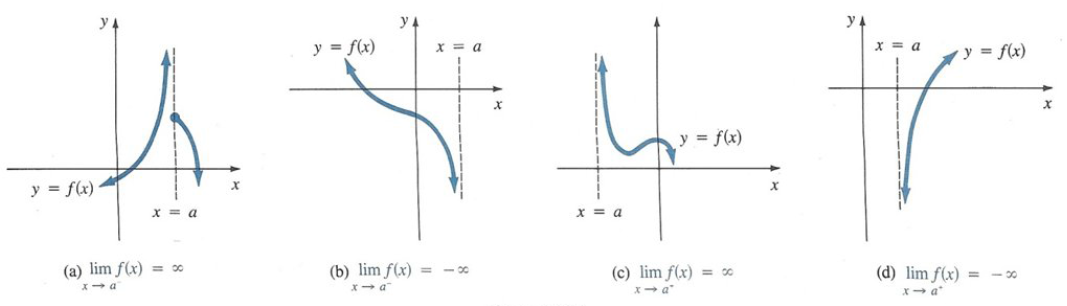
\includegraphics[width=0.89\textwidth]{in.png}\\[1cm]
  \end{center}
 
\noindent Note that $\displaystyle \lim _{x\rightarrow \infty} \dfrac{1}{x}=0$ and $\displaystyle \lim _{x\rightarrow -\infty} \dfrac{1}{x}=0$.

\subsubsection{Limits at Infinity of a Rational Function}
A rational function is a quotient of two polynomials, $f(x)=\dfrac{p_m(x)}{q_n (x)}$, where $m$ and $n$ are the degrees of the two polynomials.
\begin{enumerate}
\item \textbf{If} $m<n$, then $\displaystyle \lim _{x\rightarrow \infty}f(x)=0$.

\noindent \textbf{Example:} Find $\displaystyle \lim _{x\rightarrow \infty}\dfrac{x+1}{x^2+4} $.\\

\textbf{Solution:} The degree of the numerator is one, the degree of the denominator is two. Therefore $\displaystyle \lim _{x\rightarrow \infty}\dfrac{x+1}{x^2+4} =0$, since  $\displaystyle \lim _{x\rightarrow \infty}\dfrac{\frac{1}{x}+\frac{1}{x^2}}{1+\frac{4}{x^2}}=\dfrac{0+0}{1+0} =0$.
\item \textbf{If} $m>n$, then $\displaystyle \lim _{x\rightarrow \infty}f(x)=\pm \infty$ . (sign depends on the polynomials $p_m(x)$ and $q_n(x)$, if they are of the same sign as $x$ gets larger, the quotient is positive, if they are of opposite signs, the quotient is negative)

\textbf{Example:} Find $\displaystyle \lim _{x\rightarrow \infty}\dfrac{x^3-2x^2+3x+4}{3x+5}$.\\

\textbf{Solution:} $\displaystyle \lim _{x\rightarrow \infty}\dfrac{x^3-2x^2+3x+4}{3x+5}=\lim _{x\rightarrow \infty}\dfrac{1-\frac{2}{x}+\frac{3}{x^2}+\frac{4}{x^3}}{\frac{3}{x^2}+\frac{5}{x^3}}=\dfrac{1}{0}=\infty$.
\item \textbf{If} $m=n$, then $\displaystyle \lim _{x\rightarrow \infty}f(x)=\dfrac{a}{b}$, where $a$ is the coefficient of $x^m$ in the numerator and $b$ is the coefficient of $x^n$ in the denominator.


\textbf{Example:} Find $\displaystyle \lim _{x\rightarrow \infty}\dfrac{x^3-4x+1}{3x^3+2x+7}$.\\

\textbf{Solution:} $\displaystyle \lim _{x\rightarrow \infty}\dfrac{x^3-4x+1}{3x^3+2x+7}=\lim _{x\rightarrow \infty} \dfrac{1-\frac{4}{x^2}+\frac{1}{x^3}}{3+\frac{2}{x^2}+\frac{7}{x^3}}=\dfrac{1-0+0}{3+0+0}=\dfrac{1}{3}$.\\


\textbf{You Try It:} What is $\displaystyle \lim _{x\rightarrow \infty}\dfrac{a_0x^m+a_1x^{m-1}+\cdots + a_m}{b_0x^n+b_1x^{n-1}+\cdots +b_n}$, where $a_0, b_0 \neq 0$ and $m$ and $n$ are positive integers, when (a)\, $m>n$ \quad (b)\, $m=n$ \quad (c)\, $m<n$.

\textbf{You Try It:} Find $\displaystyle \lim _{x\rightarrow 4} \dfrac{x-4}{\sqrt{x}-2}$.
\end{enumerate}
\section{Continuity}
A function $f(x)$ is \textbf{continuous} at a point $x=a$ if 
\begin{enumerate}
\item $f(a)$ is defined.
\item $\displaystyle \lim _{x\rightarrow a} f(x)$ exists.
\item $\displaystyle \lim _{x\rightarrow a} f(x) =f(a)$.
\end{enumerate}
Notice that, for $f(x)$  to be continuous at $x=a$, all three conditions must be satisfied. If at least one condition fails, $f$ is said to have a discontinuity at $x=a$. For example, $f(x)=x^2+1$ is continuous at $x=2$ since $\displaystyle \lim _{x\rightarrow 2} f(x)=5=f(2)$. The first condition above implies that a function can be continuous only at points of its domain. Thus, $f(x)=\sqrt{4-x^2}$ is not continuous at $x=3$ because $f(3)$ is imaginary, i.e., not defined.

\noindent A function $f$ is right-continuous (continuous from the right) at a point $x=a$ in its
domain if $\displaystyle \lim _{x\rightarrow a^+}f(x)=f(a)$. It is left-continuous (continuous from the left) at $x=a$ if $\displaystyle \lim _{x\rightarrow a^-}f(x)=f(a)$. A function is continuous at an interior point $x=a$ of its domain if and only if it is both right-continuous and left-continuous at $x=a$.

\noindent \textbf{Example:} Determine whether $f(x)=x^2+1$ is continuous at $x=1$.

\noindent \textbf{Solution:} $\displaystyle \lim _{x\rightarrow 1} x^2+1=f(1)=1^2+1=2$. Therefore $f(x)=x^2+1$ is continuous at $x=1$. 

\noindent \textbf{Example:} Determine whether $f(x)=\dfrac{|x|}{x}$ is continuous at $x=0$.

\noindent \textbf{Solution:} Since $f(0)$ is not defined, $f(x)$ is not continuous at $x=0$.

\noindent \textbf{Example:} Determine whether 
 \[f(x)= \left\{ 
\begin{array}{l l}
  \dfrac{|x|}{x}, & \quad \hbox{if}~~~ x\neq 0 \\
 0, & \quad \hbox{if}~~~ x=0,\\ \end{array} \right. \]
 is continuous at $x=0$.
 
 \noindent \textbf{Solution:} $f(0)$ now defined. Then 
 
 Then $\displaystyle \lim _{x\rightarrow 0} f(x)$ must be considered in two steps, 
 \begin{eqnarray*}
 \lim _{x\rightarrow 0^-}f(x) &=& \lim _{x\rightarrow 0^-} (-1) = -1.\\
 \lim _{x\rightarrow 0^+}f(x) &=& \lim _{x\rightarrow 0^+} (1) = 1.
 \end{eqnarray*}
 Sine the limits are not the same, $\displaystyle \lim _{x\rightarrow 0} f(x)$ does not exist and $f(x)$ is not continuous at $x=0$.
 
 \noindent \textbf{You Try It:} Determine whether the function defined by 
 \[ f(x) = \left\{ 
\begin{array}{l l}
  x^2, & \quad \hbox{if}~~~ x<2 \\
  5, & \quad \hbox{if}~~~x=2\\
 -x+6, & \quad \hbox{if}~~~ x>2,\\ \end{array} \right. \]
 is continuous at the point $x=2$.
 
 
\noindent A function $f(x)$ is \textbf{discontinuous} at $x=a$ if one or more of the conditions for continuity fails there.
 
 \noindent \textbf{Example:} (a)\, $f(x)=\dfrac{1}{x-2}$ is discontinuous at $x=2$, because $f(2)$ is not defined (has a zero denominator) and because $\displaystyle \lim _{x\rightarrow 2}f(x)$ does not exist (equals $\infty$). The function is, however, continuous everywhere except at $x=2$, where it is said to have an \textit{infinite discontinuity}. 
 
 \noindent (b)\, $f(x)=\dfrac{x^2-4}{x-2}$ is discontinuous at $x=2$ because $f(2)$ is not defined (both numerator and denominator are zero) and because $\displaystyle \lim _{x\rightarrow 2}f(x)=4$. The discontinuity here is called \textit{removable} since it may be removed by redefining the function as $f(x)=\dfrac{x^2-4}{x-2}$ for $x\neq 2$ and $f(2)=4$. (Note the discontinuity in (a) cannot be removed because the limit also does not exist.)
 
 \section{The $\varepsilon - \delta$ Definition of Continuity}
 $f(x)$ is continuous at $x=a$, if for any $\varepsilon >0$, we can find $\delta >0$, such that, $|f(x)-f(a)|<\varepsilon$ whenever $0<|x-a|<\delta$.
 
 \noindent \textbf{Example:} Prove that $f(x)=x^2$ is continuous at $x=2$.
 
 \noindent \textbf{Solution:} Must show that, given any $\varepsilon >0$, we can find $\delta>0$, such that $|f(x)-f(2)|=|x^2-4|<\varepsilon$ when $|x-2|<\delta$.
 
 \noindent Choose $\delta \leq 1$, so that $|x-2|<1$ or $1<x<3$ ($x\neq 2$). Then $|x^2-4|=|(x-2)(x+2)|=|x-2||x+2| <\delta|x+2|<5\delta$. Taking $\delta =\min \{1, \frac{\varepsilon}{5}\}$ whichever is smaller, then we have $|x^2-4|<\varepsilon$ whenever $|x-2|<\delta$.
 
 
 \noindent \textbf{You Try It:} (a)\, Prove that $f(x)=x$ is continuous at any point $x=x_0$.\\
 (b)\, Prove that $f(x)=2x^3+x$ is continuous at any point $x=x_0$.
 \subsubsection{Theorems on Continuity}
 \begin{enumerate}
 \item[Theorem $1$.] If $f(x)$ and $g(x)$ are continuous at $x=a$, so are the functions $f(x) \pm g(x), \, f(x)g(x)$ and $\dfrac{f(x)}{g(x)}$ if $g(x) \neq 0$.
 \item[Theorem $2$.] The following functions are continuous in every finite interval (a)\, all polynomials \quad (b)\, $\sin x$ and $\cos x$ \quad (c)\, $a^x, a>0$.
 \item[Theorem $3$.] If $y=f(x)$ is continuous at $x=a$ and $z=g(y)$ is continuous at $y=b$ and if $b=f(a)$, then the function $z=g[f(x)]$ called a function of a function or composite function is continuous at $x=a$.
 
 \textbf{Briefly:} A continuous function of a continuous function is continuous. 
 \item[Theorem $4$.] If $f(x)$ is continuous in a closed interval, it is bounded in the interval.
\end{enumerate} 
\noindent \textbf{You Try It:} Suppose that $f(x)\leq g(x)\leq h(x)$ for all $x$ in an open interval containing  $a$ and $\displaystyle \lim _{x\rightarrow a}f(x)=\lim _{x\rightarrow a}h(x)=L$. Then, show that $\displaystyle \lim _{x\rightarrow a}g(x)=L$.
\section{Tutorial Questions}
\begin{enumerate}
\item Let \[f(x) = \left\{ 
\begin{array}{l l}
  3x-1, & \quad x< 0\\
  0, & \quad x=0\\
  2x+5, & \quad x >0,\\ \end{array} \right. \]
  Evaluate (i)\, $\displaystyle \lim _{x\rightarrow 2}f(x) $ \quad (ii)\, $\displaystyle \lim _{x\rightarrow -3}f(x)$ \quad (iii)\, $\displaystyle \lim _{x\rightarrow 0^+}f(x)$ \quad (iv)\, $\displaystyle \lim _{x\rightarrow 0^-}f(x)$ \quad (v)\, $\displaystyle \lim _{x\rightarrow 0}f(x)$.
  \item If $f(x)=\dfrac{3x+|x|}{7x-5|x|}$. Evaluate (i)\, $\displaystyle \lim _{x\rightarrow \infty}f(x)$ \quad (ii)\,$\displaystyle \lim _{x\rightarrow -\infty}f(x)$ \quad (iii)\, $\displaystyle \lim _{x\rightarrow 0^+}f(x)$ \\
   (iv)\, $\displaystyle \lim _{x\rightarrow 0^-}f(x)$ \quad (v)\, $\displaystyle \lim _{x\rightarrow 0}f(x)$
\item Use the theorems on limits to evaluate each of the following limits.\\
(i)\, $\displaystyle \lim _{x\rightarrow 0}\dfrac{x^3-8}{x-2}$ \quad (ii)\, $\displaystyle \lim _{x\rightarrow 0}{\dfrac{\sqrt{3+x}-\sqrt{3}}{{x}}}$  \quad (iii)\, $\displaystyle \lim _{x\rightarrow \infty}{\dfrac{8x^2+4}{2x^2-x+2}}$ \quad (iv)\, $\displaystyle \lim _{x\rightarrow 2}{(4x^2-x+5)}$\\
(v)\, $\displaystyle \lim _{x \rightarrow 0}{\dfrac{\sqrt{x+4}-2}{x}}$ \quad (vi)\, $\displaystyle \lim _{x\rightarrow \infty}{\dfrac{a_0+a_1x+\cdots +a_mx^m}{b_0+b_1x+\cdots +b_nx^n}}$ \quad (vii)\, $\displaystyle \lim _{x\rightarrow \infty}{\dfrac{(3x-1)(2x+3)}{(5x-3)(4x+5)}}$\\
(viii)\, $\displaystyle \lim _{x\rightarrow  0}{\dfrac{\sin 3x}{x}}$ \quad (ix)\, $\displaystyle \lim _{x\rightarrow 0}{\dfrac{6x-\sin 2x}{2x+3\sin 4x}}$ \quad (x)\, $\displaystyle \lim _{x\rightarrow 0}{\dfrac{\sin x}{\sin 2x}}$ \quad (xi)\, $\displaystyle \lim _{x\rightarrow 4}{\dfrac{2x-8\sqrt{x}+8}{\sqrt{x}-2}}$.
\item For $f(x)=5x-6$, find a $\delta >0$ such that  whenever $0<|x-4|<\delta$, then $|f(x)-14|<\varepsilon$ when (i)\, $\varepsilon =\frac{1}{2}$ \quad (ii)\, $\varepsilon =0.001$.
\item Verify (i)\, $\displaystyle \lim _{x\rightarrow 2}\dfrac{x^2-4}{x-2}=4$ \quad (ii)\, $\displaystyle \lim _{x\rightarrow 0}x^2 \cos \left(\frac{1}{x}\right)=0$.
\item Give the points of discontinuity of each of the following functions.\\
(i)\, $f(x)=\dfrac{x}{(x-2)(x-4)}$ \quad (ii)\, $f(x)=x^2\sin \left(\frac{1}{x}\right), f(0)=0$ \\
(iii)\, $f(x)=\sqrt{(x-3)(6-x)}, 3 \leq x\leq 6$ \quad (iv)\, $f(x)=\dfrac{1}{1+2\sin x}$.
\item For what values of $x$ in the domain of definition is each of the following functions continuous?\\
(i)\, $f(x)=\dfrac{x}{x^2-1}$ \quad (ii)\, $f(x)=\dfrac{1+\cos x}{3+\sin x }$ \quad (iii)\, $f(x)=10^{-\frac{1}{(x-3)^2}}$ \\ (iv)\, $f(x)=\dfrac{x-|x|}{x}$.
\item Given that the function $f:\mathbb{R} \to \mathbb{R}$ be defined by
\[f(x) = \left\{ 
\begin{array}{l l}
  x^2-4, & \quad x \geq 2\\
  2ax+b, & \quad 0<x<2\\
  e^x, & \quad x\leq 0,\\ \end{array} \right. \] 
  is continuous at all points in $\mathbb{R}$. Find the values of $a$ and $b$.
  \item Find the values of $a$ and $b$ such that the function $f$ will be continuous on $\mathbb{R}$
  \[f(x) = \left\{ 
\begin{array}{l l}
  ax-3, & \quad x< 2\\
  3-x-2x^2, & \quad 2\leq x \leq 4\\
  bx+7, & \quad x >4.\\ \end{array} \right. \]
\item  Determine all values of the the constant $A$ so that the following is continuous for all values of $x$, 
\[f(x) = \left\{ 
\begin{array}{l l}
  A^2x-A, & \quad x \geq 3\\
  4, & \quad x <3.\\ \end{array} \right. \] 
\item Determine all the values of the constants $A$ and $B$ so that the following is continuous for all values of $x$,
\[f(x) = \left\{ 
\begin{array}{l l}
  Ax-B, & \quad x\leq -1\\
  2x^2+3Ax+B, & \quad -1<x\leq 1\\
  4, & \quad x >1.\\ \end{array} \right. \]
  \item The function $f:\mathbb{R} \to \mathbb{R}$ is defined by 
  \[f(x) = \left\{ 
\begin{array}{l l}
 \sin x, & \quad x\leq 0\\
  ax+b, & \quad 0<x \leq 3\\
  x^3, & \quad x >3.\\ \end{array} \right. \]
  Find all the values of $a$ and $b$ if $f$ is continuous on $\mathbb{R}$.
  \item Let $f:\mathbb{R} \to \mathbb{R}$ be the function defined by 
  \[f(x) = \left\{ 
\begin{array}{l l}
  x^2, & \quad x\geq 2\\
  ax+b, & \quad 1<x<2\\
  2-x, & \quad x\leq 1,\\ \end{array} \right. \]
  where $a$ and $b$ are constants. If $f$ is continuous on $\mathbb{R}$, find the values $a$ and $b$.
\end{enumerate}
\chapter{Differentiation}
\begin{center}
	\small{\parbox{18cm}{
		\begin{raggedright}
		{\small
		\textit{Any man who can drive safely while kissing a pretty girl is simply not giving the kiss the attention it deserves.}
 }
 
				\vspace{.5cm}\hfill{---Albert Einstein }
		\end{raggedright}
	}
} 
\end{center}
\textbf{Increments.} The \textit{increment} $\Delta x$ of a variable $x$ is the change in $x$ as it increases or decreases from one value $x=x_0$ to another value $x=x_1$ in its domain. Here, $\Delta x=x_1-x_0$ and we may write $x_1=x_0+\Delta x$. If the variable $x$ is given an increment $\Delta x$ from $x=x_0$ (i.e., if $x$ changes from $x=x_0$ to $x_1=x_0+\Delta x$) and a function $y=f(x)$ is thereby given an increment $\Delta y=f(x_0+\Delta x)-f(x_0)$ from $y=f(x_0)$, then the quotient 
\begin{equation*}
\dfrac{\Delta y} {\Delta x}=\dfrac{\hbox{change in}~~ y}{\hbox{change in }~ x}, 
\end{equation*}
is called the \textit{average rate of change} of the function on the interval between $x=x_0$ and $x_1=x_0+\Delta x$.
 
\noindent Let $f(x)$ be defined at any point $x_0$ in $(a,b)$. The derivative of $f(x)$ at $x=x_0$ is defined as 
\begin{equation*}
f'(x_0)=\lim _{h\rightarrow 0}\dfrac{f(x_0+h)-f(x_0)}{h}
\end{equation*}
if this limit exists. A function is called \textbf{differentiable} at a point $x=x_0$, if it has a derivative at that point, i.e., if $f'(x_0)$ exists.  If we write $x=x_0+h$, then $h=x-x_0$ and $h$ approaches $0$ if and only if $x$ approaches $x_0$. Therefore, an equivalent way of stating the definition of the derivative, is 
\begin{equation*}
f'(x_0)=\lim _{x\rightarrow x_0} \dfrac{f(x)-f(x_0)}{x-x_0}.
\end{equation*}

\noindent \textbf{Example:} If $f(x)=x^3-x$, find a formula for $f'(x)$.

\noindent \textbf{Solution:} 
\begin{eqnarray*}
f'(x) &=& \lim _{h\rightarrow 0} \dfrac{f(x+h)-f(x)}{h} =\lim _{h\rightarrow 0}\dfrac{[(x+h)^3-(x+h)]-[x^3-x]}{h}\\
&=& \lim _{h\rightarrow 0} \dfrac{x^3+3x^2h+3xh^2+h^3-x-h-x^3+x}{h}\\
&=& \lim _{h\rightarrow 0} \dfrac{3x^2h+3xh^2+h^3-h}{h}\\
&=& \lim _{h\rightarrow 0} (3x^2+3xh+h^2-1) =3x^2-1.
\end{eqnarray*}

\noindent \textbf{Example:} If $f(x)=\sqrt{x}$, find the derivative of $f$.

\noindent \textbf{Solution:} 
\begin{eqnarray*}
f'(x) &=& \lim _{h\rightarrow 0} \dfrac{f(x+h)-f(x)}{h}\\
&=& \lim _{h\rightarrow 0} \dfrac{\sqrt{x+h}-\sqrt{x}}{h}\\
&=& \lim _{h\rightarrow 0} \dfrac{\sqrt{x+h}-\sqrt{x}}{h} \cdot \dfrac{\sqrt{x+h}+\sqrt{x}}{\sqrt{x+h}-\sqrt{x}}\\
&=& \lim _{h\rightarrow 0} \dfrac{(x+h)-x}{h(\sqrt{x+h}+\sqrt{x})}\\
&=& \lim _{h\rightarrow 0} \dfrac{1}{\sqrt{x+h}+\sqrt{x}}\\
&=& \dfrac{1}{\sqrt{x} +\sqrt{x}} =\dfrac{1}{2\sqrt{x}}. 
\end{eqnarray*}
\noindent The derivative at $x$ may be denoted by $f'(x)$, $y'$, $\dfrac{dy}{dx}$, $\dfrac{d}{dx}(f(x))$. The symbol $\dfrac{d}{dx}$ is called \textbf{differentiation operator} because it indicates the operation of \textbf{differentiation}. The process of finding derivatives of functions is called \textbf{differentiation}.

\noindent  A function $f$ is differentiable at $x_0$ if $f'(x_0)$ exists. It is \textbf{differentiable on an open interval} $(a,b)$ [or $(a,\infty)$ or $(-\infty , a)$ or $(-\infty , \infty)$], if it is differentiable at every number in the interval.

\noindent \textbf{Example:} Where is the function $f(x)=|x|$ differentiable?

\noindent \textbf{Solution:} If $x>0$, then $|x|=x$ and we can choose $h$ small enough that $x+h>0$ and hence $|x+h|=x+h$. Therefore, for $x>0$, 
\begin{eqnarray*}
f'(x) &=& \lim _{h\rightarrow 0}\dfrac{|x+h|-|x|}{x}\\
&=&\lim _{h\rightarrow 0} \dfrac{(x+h)-x}{h}=\lim _{h\rightarrow 0}\dfrac{h}{h}=1,
\end{eqnarray*}
and so $f$ is differentiable for any $x>0$. 

\noindent Similarly, for $x<0$, we have $|x|=-x$ and $h$ can be chosen small enough that $x+h<0$ and so $|x+h|=-(x+h)$. Therefore, for $x<0$, 
\begin{eqnarray*}
f'(x) &=& \lim _{h\rightarrow 0}\dfrac{|x+h|-|x|}{h}\\
&=& \lim _{h\rightarrow 0}\dfrac{-(x+h)-(-x)}{h} =\lim _{h\rightarrow 0} \dfrac{-h}{h}=-1,
\end{eqnarray*} 
and so $f$ is differentiable for any $x<0$. 

\noindent For $x=0$ we have to investigate 
\begin{eqnarray*}
f'(0) &=& \lim _{h\rightarrow 0}\dfrac{f(0+h)-f(0)}{h}\\
&=& \lim _{h\rightarrow 0} \dfrac{|0+h|-|0|}{h} \quad (\hbox{if it exists}). 
\end{eqnarray*}
Let's compute the left and right limits separately;
\begin{eqnarray*}
\lim _{h\rightarrow 0^+} \dfrac{|0+h|-|0|}{h} &=& \lim _{h\rightarrow 0^+}\dfrac{|h|}{h}=\lim _{h\rightarrow 0^+} 1=1.\\
\lim _{h\rightarrow 0^-} \dfrac{|0+h|-|0|}{h} &=& \lim _{h\rightarrow 0^-}\dfrac{|h|}{h}=\lim _{h\rightarrow 0^-} (-1)=-1.
\end{eqnarray*}
Since these limits are different $f'(0)$ does not exist.  Thus, $f$ is differentiable at all $x$ except $0$.
\section{Differentiation Techniques (Finding Derivatives)}
\begin{enumerate}
\item \begin{equation*}
f'(x_0)=\lim _{h\rightarrow 0}\dfrac{f(x_0+h)-f(x_0)}{h}
\end{equation*}
if this limit exists.
\item The derivative of any constant function is zero, i.e., $c'=0$.
\item For any real number $n$, 
\begin{equation*}
(x^n)'=nx^{n-1}.
\end{equation*}
When differentiating, results can be expressed in a number of ways. For example, (i)\, if $y=3x^2$ then $\dfrac{dy}{dx}=6x$, \quad (ii)\, if $f(x)=3x^2$ then $f'(x)=6x$, \quad (iii)\, the differential coefficient of $3x^2$ is $6x$. \\
For example, if $f(x)=\sqrt{x}=x^{\frac{1}{2}}$, then $f'(x)=\dfrac{1}{2}x^{\frac{1}{2}-1}=\frac{1}{2}x^{-\frac{1}{2}}=\dfrac{1}{2\sqrt{x}}$.\\
\textbf{You Try It:} Using the general rule, differentiate the following with respect to $x$ :\\ (a)\, $f(x)=5x^7$ \quad (b)\, $f(x)=\dfrac{4}{x^2}$.
\item For any constant $c$, $(cf(x))'=cf'(x)$. For example, $(5x^3)'=5(x^3)'=5(3x^2)=15x^2$.
\item The derivative of a sum (difference) is the sum (difference) of the derivatives, 
\begin{equation*}
(f(x)\pm g(x))'=f'(x)\pm g'(x).
\end{equation*}
For example, \[(3x^5-2x^2+1)'=(3x^5)'-(2x^2)'+1'=3(x^5)'-2(x^2)'+0=3(5x^4)-2(2x)=15x^4-4x.\]
\item Product Rule 
\begin{equation*}
(f(x)g(x))'=f(x)g'(x)+g(x)f'(x).
\end{equation*}
\item Quotient Rule
\begin{equation*}
\left(\dfrac{f(x)}{g(x)}\right)'=\dfrac{g(x)f'(x)-f(x)g'(x)}{(g(x))^2}.
\end{equation*}
\item \textbf{Parametric Equations.} If the coordinates $(x,y)$ of a point $P$ on a curve are given as functions $x=f(u)$ and $y=g(u)$ of a third variable or \textit{parameter} $u$, the equations $x=f(u)$ and $y=g(u)$ are called \textit{parametric equations of the curve}. For example, $x=\frac{1}{2}t, \, y=4-t^2$ or $x=\cos \theta, \, y=4\sin ^2 \theta$.

\noindent \textbf{The First Derivative} $\dfrac{dy}{dx}$ is given by 
\begin{equation*}
\dfrac{dy}{dx} =\dfrac{dy/ du}{dx/ du}.
\end{equation*}
\textbf{The Second Derivative} $\dfrac{d^2y }{dx^2}$ is given by 
\begin{equation*}
\dfrac{d^2y}{dx^2} =\dfrac{d}{du}\left( \dfrac{dy}{dx}\right)\dfrac{du}{dx}.
\end{equation*}
\textbf{Example:} Find $\dfrac{dy}{dx}$ and $\dfrac{d^2y}{dx^2}$ given $x=\theta-\sin \theta$ and $y=1-\cos \theta$.

\noindent \textbf{Solution:} Note that $\dfrac{dx}{d\theta}=1-\cos \theta$ and $\dfrac{dy}{d\theta}=\sin \theta$, so 
\begin{equation*}
\dfrac{dy}{dx} =\dfrac{dy/ d\theta}{dx/ d\theta}=\dfrac{\sin \theta}{1-\cos \theta}.
\end{equation*}
Also \begin{eqnarray*}
\dfrac{d^2y}{dx^2} &=& \dfrac{d}{d\theta}\left( \dfrac{\sin \theta}{1-\cos \theta}\right)\dfrac{d\theta}{dx}\\
&=& \dfrac{\cos \theta -1}{(1-\cos \theta)^2}\cdot \dfrac{1}{1-\cos \theta} =-\dfrac{1}{(1-\cos \theta)^2}.
\end{eqnarray*}
\textbf{Example:} Find $\dfrac{dy}{dx}$ and $\dfrac{d^2y}{dx^2}$ given $x=e^t\cos t$ and $y=e^t\sin t$.

\noindent \textbf{Solution:} Note that $\dfrac{dx}{dt}=e^t(\cos t -\sin t)$ and $\dfrac{dy}{dt}=e^t(\sin t +\cos t)$, so 
\begin{equation*}
\dfrac{dy}{dx} =\dfrac{dy/ dt}{dx/ dt}=\dfrac{\sin t +\cos t}{\cos t -\sin t}.
\end{equation*}
Also 
\begin{eqnarray*}
\dfrac{d^2y}{dx^2} &=& \dfrac{d}{dt}\left(\dfrac{\sin t +\cos t}{\cos t -\sin t} \right)\dfrac{dt}{dx}\\
&=& \dfrac{2}{(\cos t - \sin t)^2} \cdot \dfrac{1}{e^t(\cos t -\sin t)} =\dfrac{2}{e^t(\cos t -\sin t)^3}.
\end{eqnarray*}
\end{enumerate}
\begin{theorem}
If $f(x)=c$ is a constant function, then $f'(x)=0$ for all real numbers $x$. 
\end{theorem}
\begin{proof}
Observe that $f'(x)=\displaystyle \lim _{h\rightarrow 0}\dfrac{f(x+h)-f(x)}{h}=\displaystyle \dfrac{c-c}{h}=0$.
\end{proof}
\begin{theorem}[Product Rule]
If $f$ and $g$ are both differentiable at $x$, then the product function $fg$ is also differentiable at $x$ and $(fg)'(x)=f(x)g'(x)+g(x)f'(x)$.
\end{theorem}
\begin{proof}
\begin{equation*}
(fg)'(x)=\lim _{h\rightarrow 0}\dfrac{f(x+h)g(x+h)-f(x)g(x)}{h}.
\end{equation*}
Trick of adding and subtracting $f(x+h)g(x)$ to the numerator,
\begin{eqnarray*}
\lim _{h\rightarrow 0}\dfrac{f(x+h)g(x+h)-f(x+h)g(x)+f(x+h)g(x)-f(x)g(x)}{h} &=&\\
\lim _{h\rightarrow 0} {f(x+h)}\lim _{h\rightarrow 0}\dfrac{g(x+h)-g(x)}{h}+g(x)\lim _{h\rightarrow 0}\dfrac{f(x+h)-f(x)}{h} &=&\\
f(x)g'(x)+g(x)f'(x).
\end{eqnarray*}
\end{proof}
\begin{theorem}
If $g$ is differentiable at $x$ and $g(x)\neq 0$, then 
\begin{equation*}
\left(\dfrac{1}{g}\right)'(x)=-\dfrac{g'(x)}{(g(x))^2}.
\end{equation*}
\end{theorem}
\begin{proof}
\begin{eqnarray*}
\lim _{h\rightarrow 0} \dfrac{\frac{1}{g(x+h)}-\frac{1}{g(x)}}{h} &=& \lim _{h\rightarrow 0}\dfrac{g(x)-g(x+h)}{h(g(x))(g(x+h))}\\
&=& \lim _{h\rightarrow 0} \dfrac{-(g(x+h)-g(x))}{h}\dfrac{1}{g(x)g(x+h)}\\
&=& \lim _{h\rightarrow 0} \dfrac{-(g(x+h)-g(x))}{h} \lim _{h\rightarrow 0}\dfrac{1}{g(x)g(x+h)}\\
&=& -g'(x)\dfrac{1}{(g(x))^2}.
\end{eqnarray*}
\end{proof}
\begin{theorem}
If $f$ and $g$ are differentiable at $x$ and $g(x)\neq 0$, then $\dfrac{f}{g}$ is differentiable at $x$ and 
$\left(\dfrac{f}{g}\right)'(x)=\dfrac{g(x)f'(x)-f(x)g'(x)}{(g(x))^2} $.
\end{theorem}
\begin{proof}
Since $\dfrac{f}{g}=f\left(\dfrac{1}{g}\right)$, we have
\begin{eqnarray*}
\left(\dfrac{f}{g}\right)'(x) &=&\left(f\cdot \dfrac{1}{g}\right)'(x)\\
&=& f'(x)\dfrac{1}{g(x)}+f(x)\left(\dfrac{1}{g}\right)'(x)\\
&=& \dfrac{f'(x)}{g(x)}+f(x)\left(-\dfrac{g'(x)}{(g(x))^2}\right)\\
&=& \dfrac{f'(x)g(x)-f(x)g'(x)}{(g(x))^2}.
\end{eqnarray*}
\end{proof}
\textbf{Example:} $f(x)=\dfrac{x^2-1}{x^2+1}$, then $f'(x)=\dfrac{(x^2+1)(2x)-(x^2-1)(2x)}{(x^2+1)^2}=\dfrac{4x}{(x^2+1)^2}$.

\noindent \textbf{Example:} If $f(x)=\dfrac{x}{x^2+1}$, then $f'(x)=\dfrac{(x^2+1)-x(2x)}{(x^2+1)^2}=\dfrac{1-x^2}{(x^2+1)^2}$.

\noindent \textbf{Example:} If $f(x)=\dfrac{1}{x}$, then $f'(x)=-\dfrac{1}{x^2}$.

\noindent \textbf{Example:} If $x=\cos t$ and $y=t\sin t$, find $\dfrac{dy}{dx}$.

\noindent \textbf{Solution:} \begin{equation*}
\dfrac{dy}{dx}=\dfrac{\dfrac{d}{dt}(t\sin t)}{\dfrac{d}{dt}(\cos t)}=\dfrac{\sin t+t\cos t}{-\sin t}.
\end{equation*}
\section{Derivatives of Trigonometric Functions}
Recall : 
\begin{equation*}
\lim _{h\rightarrow 0} \dfrac{\sin h}{ h}=1 \quad \hbox{and} \quad \lim _{h\rightarrow 0} \dfrac{1-\cos h}{h}=0.
\end{equation*}
\begin{eqnarray*}
(\sin x)' &=& \lim _{h\rightarrow 0} \dfrac{\sin (x+h)-\sin x}{h}\\
&=& \lim _{h\rightarrow 0} \dfrac{\sin x \cos h +\cos x \sin h -\sin x}{h}\\
&=& \lim _{h\rightarrow 0} \dfrac{\sin x (\cos h-1)+\cos x \sin h}{h}\\
&=& \lim _{h\rightarrow 0} \left(-\sin x \dfrac{(1-\cos h)}{h}+\left(\cos x\dfrac{\sin h}{h}\right)\right)\\
&=& -\sin x (0)+\cos x (1).
\end{eqnarray*}
Hence $(\sin x)'=\cos x$.

\noindent \textbf{Example:} Find $\dfrac{dy}{dx}$ if $y=x^3\sin x$.

\noindent \textbf{Solution:} $\dfrac{dy}{dx}=(x^3\sin x)'=x^3(\sin x)'+\sin x (x^3)'=x^3\cos x +3x^2\sin x$.

\noindent \textbf{Example:} Determine whether the function, 
\[ f(x) = \left\{ 
\begin{array}{l l}
  x^3\sin \left(\dfrac{1}{x}\right), & \quad \hbox{if}~~~ x\neq 0 \\
 0, & \quad \hbox{if}~~~ x=0,\\ \end{array} \right. \]
 is differentiable at $x=0$.
 
\noindent \textbf{Solution:}  Observe that 
\begin{equation*}
\lim _{h\rightarrow 0} \dfrac{h^3\sin \frac{1}{h}-0}{h}=\lim _{h\rightarrow 0}h^2\sin \frac{1}{h}=0.
\end{equation*}

\noindent \textbf{Logarithmic Functions.} Assume $a>0$ and $a\neq 1$. If $a^y=x$, then define $y=\log _a x$. Let $\ln x \equiv \log _e x$ ($\ln x$ is called the \textit{natural logarithm} of $x$).

\noindent \textbf{Basic Properties of Logarithms}
\begin{enumerate}
\item $\log _a 1 =0$ (In particular, $\ln 1 =0$).
\item $\log _a a=1$ (In particular, $\ln e =1$).
\item $\log _a uv=\log _a u +\log _a v$.
\item $\log _a \left(\dfrac{u}{v}\right)=\log _a u-\log _a v$.
\item $\log _a u^r =r\log _a u$.
\end{enumerate}

\noindent \textbf{Derivatives of $\ln x$ and $e^x$} are $\dfrac{d}{dx}e^x=e^x$ and $\dfrac{d}{dx}\ln x =\dfrac{1}{x}$. Also $\dfrac{d}{dx}(a^x)=a^x\ln x, \, a>0$.

\noindent \textbf{Example:} Calculate the derivative $\dfrac{d}{dx}[(\sin x +x)\cdot (x^3-\ln x)]$.

\noindent \textbf{Solution:}  We know that $\dfrac{d}{dx} \sin x =\cos x, \dfrac{d}{dx} x=1, \, \dfrac{d}{dx}x^3=3x^2$ and $\dfrac{d}{dx}\ln x =\dfrac{1}{x}$. Therefore, by the addition rule, 
\begin{equation*}
\dfrac{d}{dx} (\sin x +x) =\dfrac{d}{dx}\sin x +\dfrac{d}{dx} x =\cos x +1
\end{equation*} 
and 
\begin{equation*}
\dfrac{d}{dx} (x^3-\ln x)=\dfrac{d}{dx}x^3-\dfrac{d}{dx}\ln x =3x^2-\dfrac{1}{x}.
\end{equation*}
Now we may conclude the calculation by applying the product rule;
\begin{eqnarray*}
\dfrac{d}{dx}[(\sin x +x)\cdot(x^3-\ln x)] &=& \dfrac{d}{dx} (\sin x +x)\cdot (x^3-\ln x) +(\sin x +x)\cdot \dfrac{d}{dx}(x^3-\ln x)\\
&=& (\cos x +1)\cdot (x^3-\ln x) +(\sin x +x)\cdot \left(3x^2-\dfrac{1}{x}\right)\\
&=& 4x^3-1 +x^3\cos x +3x^2\sin x -\dfrac{1}{x}\sin x -\ln x \cos x -\ln x. 
\end{eqnarray*}

\noindent \textbf{You Try It:} Calculate the derivative 
\begin{equation*}
\dfrac{d}{dx}\left(\sin x \cdot \left( \cos x -\dfrac{x}{e^x+\ln x}\right)\right).
\end{equation*}
\section{Derivative of a Composition [The Chain Rule]}
We calculate the derivative of a composition by 
\begin{equation*}
[f\circ g(x)]'=f'(g(x))\cdot g'(x).
\end{equation*}
If $y=f(u)$ where $u=g(x)$, then 
\begin{equation*}
\dfrac{dy}{dx}=\dfrac{dy}{du}\cdot \dfrac{du}{dx}=f'(u)\dfrac{du}{dx}=f'(g(x))g'(x).
\end{equation*}
Similarly, if $y=f(u)$ where $u=g(v)$ and $v=h(x)$, then 
\begin{equation*}
\dfrac{dy}{dx}=\dfrac{dy}{du}\cdot \dfrac{du}{dv}\cdot \dfrac{dv}{dx}.
\end{equation*}

\noindent \textbf{Example:} Calculate the derivative $\dfrac{d}{dx}(\sin (x^3-x^2))$.

\noindent \textbf{Solution:}  This is the composition of functions, so we must apply the Chain Rule.  It is essential to recognize what function will play the role of $f$ and what function will play the role of $g$. Notice that, if $x$  is the variable, then $x^3-x^2$ is applied first and $\sin$ applied next. So it must be that $g(x)=x^3-x^2$ and $f(s)=\sin s$. Notice that $\dfrac{d}{ds}f(s)=\cos s$ and $\dfrac{d}{dx}g(x)=3x^2-2x$. Then 
\begin{equation*}
\sin (x^3-x^2) =f\circ g(x)
\end{equation*}
and \begin{eqnarray*}
\dfrac{d}{dx}(\sin (x^3-x^2)) &=& \dfrac{d}{dx}(f\circ g(x))\\
&=& \left[\dfrac{df}{ds}(g(x)) \right]\cdot \dfrac{d}{dx}g(x)\\
&=& \cos (g(x)) \cdot (3x^2-2x)\\
&=& [\cos (x^3-x^2)]\cdot (3x^2-2x).
\end{eqnarray*}

\noindent \textbf{Example:} Calculate the derivative $\dfrac{d}{dx}\ln \left(\dfrac{x^2}{x-2}\right)$.

\noindent \textbf{Solution:} Let $h(x)=\ln \left(\dfrac{x^2}{x-2}\right)$. Then $h=f\circ g$, where $f(s)=\ln s$ and $g(x)=\dfrac{x^2}{x-2}$.  So $\dfrac{d}{ds}f(s)=\dfrac{1}{s}$ and $\dfrac{d}{dx} g(x)=\dfrac{(x-2)\cdot 2x-x^2\cdot 1}{(x-2)^2}=\dfrac{x^2-4x}{(x-2)^2}$. As a result, 
\begin{eqnarray*}
\dfrac{d}{dx}h(x) &=& \dfrac{d}{dx} (f\circ g)\\
&=& \left[\dfrac{df}{ds}(g(x)) \right]\cdot \dfrac{d}{dx}g(x)\\
&=& \dfrac{1}{g(x)}\cdot \dfrac{x^2-4x}{(x-2)^2}\\
&=& \dfrac{1}{\dfrac{x^2}{x-2}} \cdot \dfrac{x^2-4x}{(x-2)^2}\\
&=& \dfrac{x-4}{x(x-2)}.
\end{eqnarray*}

\noindent \textbf{You Try It:} Calculate the derivative of $\tan (e^x-x)$.
\section{Continuity and Differentiation}
What is the relationship between continuity and differentiation? It appears that functions that have derivatives must be continuous.
\begin{theorem}
If a function  $f$ is differentiable at a point $x$, then it is continuous at $x$.
\end{theorem}
\begin{proof}
We want to show that $f$ is continuous at $x$, i.e., $\displaystyle \lim _{t\rightarrow x} f(t)=f(x)$ or $\displaystyle \lim _{h\rightarrow 0} f(x+h)=f(x)$, where $h=t-x$. It will be sufficient to show that $\displaystyle \lim _{h\rightarrow 0} [f(x+h)-f(x)]=0$.

\noindent Now, 
\begin{eqnarray*}
\lim _{h\rightarrow 0} [f(x+h)-f(x)] &=& \lim _{h\rightarrow 0} \left[\dfrac{f(x+h)-f(x)}{h}\right]h\\
&=& \lim _{h\rightarrow 0} \dfrac{f(x+h)-f(x)}{h} \lim _{h\rightarrow 0} h \\
&=& f'(x)\cdot 0 \\
&=& 0, 
\end{eqnarray*}
because $f'(x)$ is finite. Thus $f$ is continuous at $x$.
\end{proof}
\noindent \textbf{Converse is false:} For example, the function $f(x)=|x|$ is continuous at $x=0$, but it is not differentiable there. 

\section{Higher Order Derivatives}
If $f(x)$ is differentiable in an interval, its derivative is given by $f'(x), \, y'$ or $\dfrac{dy}{dx}$ where $y=f(x)$.

\noindent If $f'(x)$ is also differentiable in the interval, its derivative is denoted by $f''(x), \, y''$ or $\dfrac{d}{dx}\left(\dfrac{dy}{dx}\right)=\dfrac{d^2y}{dx^2}$.

\noindent Similarly, the $nth$ derivative of $f(x)$, if it exists, is denoted by $f^{(n)}, \, y^{(n)}$ or $\dfrac{d^ny}{dx^n}$ where $n$ is called the order of the derivative.

\noindent \textbf{Example:} Let $y=f(x)=\frac{1}{2}x^4-3x^2+1$.

\noindent \textbf{Solution:} Derivative $y'=f'(x)=\dfrac{d}{dx}(\frac{1}{2}x^4-3x^2+1)=2x^3-6x$.

\noindent Second derivative $y''=f''(x)=\dfrac{d^2y}{dx^2}=\dfrac{d}{dx}(2x^3-6x)=6x^2-6$.

\noindent Third derivative $y'''=f'''(x)=\dfrac{d^3y}{dx^3}=\dfrac{d}{dx}(6x^2-6)=12x$.

\noindent Fourth derivative $y^{(4)}=f^{(4)}(x)=\dfrac{d^4y}{dx^4}=\dfrac{d}{dx}(12x)=12$.
\section{Implicit Differentiation}
Compare 
\begin{enumerate}
\item $x^2 -y^3 =3 \Longleftrightarrow y=\sqrt[3]{x^2-3}$.
\item $x^2+y^2=1 \Longleftrightarrow y=\pm \sqrt{1-x^2}$.
\item $x^3+y^2=3xy \Longleftrightarrow ????????$.
\end{enumerate}  
\textbf{Implicit Functions.} A function in which the dependent variable is expressed solely in terms of the independent variable $x$, namely $y=f(x)$, is said to be an \textbf{explicit function}, for example, $y=\frac{1}{2}x^3-1$. An equation $f(x,y)=0$, on perhaps certain restricted ranges of the variables, is said to define \textit{$y$ implicitly} as a function of $x$.

\noindent \textbf{Example:} (a)\, The equation $xy +x-2y-1=0$, with $x\neq 2$, defines the function $y=\dfrac{1-x}{x-2}$. \quad (b)\, The equation $4x^2+9y^2-36=0$ defines the function $y=\frac{2}{3}\sqrt{9-x^2}$ when $|x|\leq 3$ and $y\geq 0$ and the function $y=-\frac{2}{3}\sqrt{9-x^2}$ when $|x|\leq 3$ and $y\leq 0$.

\noindent The derivative $y'$ may be obtained by one of the following procedures:
\begin{enumerate}
\item Solve, when possible, for $y$ and differentiate with respect to $x$. 
\item Thinking of $y$ as a function of $x$, differentiate both sides of the given equation with respect to $x$ and solve the resulting relation for $y'$. This differentiation process is known as \textit{implicit differentiation}.
\end{enumerate}
\textbf{Example:} Find $\dfrac{dy}{dx}$ if $x^2+y^2=4$.

\noindent \textbf{Solution:} We differentiate both sides of the equation 
\begin{eqnarray*}
\dfrac{d}{dx}x^2 +\dfrac{d}{dx}y^2 &=& \dfrac{d}{dx} 4\\
2x +2y\dfrac{dy}{dx} &=0&.
\end{eqnarray*}
Solving the derivative yields
\[\dfrac{dy}{dy}=-\dfrac{x}{y}.\]

\noindent \textbf{Example:} Find $\dfrac{d^2y}{dx^2}$ if $x^2+y^2=4$.

\noindent \textbf{Solution:} From the above example, we already know that the first derivative is 
\[\dfrac{dy}{dx}=-\dfrac{x}{y}.\]
Hence by the Quotient Rule
\begin{eqnarray*}
\dfrac{d^2y}{dx^2}  &=& -\dfrac{d}{dx}\left(\dfrac{x}{y}\right)\\
&=& -\dfrac{y\cdot 1-x\cdot \dfrac{dy}{dx}}{y^2}\\
&=& -\dfrac{y-x\left(-\dfrac{x}{y}\right)}{y^2} \quad \hbox{\fbox{Substituting for $\dfrac{dy}{dx}$}}\\
&=& -\dfrac{y^2+x^2}{y^3}.
\end{eqnarray*}
Noting that $x^2+y^2=4$ permits us to write the second derivative as 
\[\dfrac{d^2y}{dx^2}=-\dfrac{4}{y^3}.\]


\noindent \textbf{Example:} Find $\dfrac{dy}{dx}$ if $\sin y=y\cos 2x$.

\noindent \textbf{Solution:} 
\begin{eqnarray*}
\dfrac{d}{dx}\sin y &=& \dfrac{d}{dx}y\cos 2x\\
\cos y \dfrac{dy}{dx} &=& y(-\sin 2x \cdot 2)+\cos 2x \dfrac{dy}{dx}\\
(\cos y-\cos 2x)\dfrac{dy}{dx} &=& -2y\sin 2x\\
\dfrac{dy}{dx} &=& -\dfrac{2y\sin 2x}{\cos y-\cos 2x}.
\end{eqnarray*}
\noindent \textbf{Example:} Find $y'$, given $xy+x-2y-1=0$.

\noindent \textbf{Solution:} We have 
\begin{equation*}
x\dfrac{d}{dx}(y)+y\dfrac{d}{dx}(x)+\dfrac{d}{dx}(x)-2\dfrac{d}{dx}(y)-\dfrac{d}{dx}(1)=\dfrac{d}{dx}(0)
\end{equation*}
or 
$xy'+y+1-2y'=0$, then $y'=\dfrac{1+y}{2-x}$.

\noindent \textbf{Example:} Find $y'$, given $x^2y-xy^2+x^2+y^2=0$.

\noindent \textbf{Solution:} 
\begin{eqnarray*}
\dfrac{d}{dx}(x^2y)-\dfrac{d}{dx}(xy^2)+\dfrac{d}{dx}(x^2)+\dfrac{d}{dx}(y^2) &=& 0\\
x^2\dfrac{d}{dx}(y)+y\dfrac{d}{dx}(x^2)-x\dfrac{d}{dx}(y^2)-y^2\dfrac{d}{dx}(x)+\dfrac{d}{dx}(x^2)+\dfrac{d}{dx}(y^2) 
&=& 0.
\end{eqnarray*}
Hence, $x^2y'+2xy-2xyy'-y^2+2x+2yy'=0$ and $y'=\dfrac{y^2-2x-2xy}{x^2+2y-2xy}$.

\noindent \textbf{Example:} Find $y'$ and $y''$, given $x^2-xy+y^2=3$.

\noindent \textbf{Solution:} 
\begin{equation*}
\dfrac{d}{dx}(x^2)-\dfrac{d}{dx}(xy)=\dfrac{d}{dx}(y^2)=2x-xy'-y+2yy'=0. \quad \hbox{So} \quad  y'=\dfrac{2x-y}{x-2y}.
\end{equation*}
Then 
\begin{eqnarray*}
y''=\dfrac{(x-2y)\dfrac{d}{dx}(2x-y)-(2x-y)\dfrac{d}{dx}(x-2y)}{(x-2y)^2} &=& \dfrac{(x-2y)(2-y')-(2x-y)(1-2y')}{(x-2y)^2}\\
&=& \dfrac{3xy'-3y}{(x-2y)^2} = \dfrac{3x\left(\dfrac{2x-y}{x-2y}\right)-3y}{(x-2y)^2} =\dfrac{6(x^2-xy+y^2)}{(x-2y)^2}\\
&=& \dfrac{18}{(x-2y)^2}.
\end{eqnarray*}

\noindent \textbf{You Try It:} Find $y''$, given $x^3-3xy+y^3=1$.

\section{Logarithmic Differentiation}
Take natural logarithm ($\ln$) both sides, differentiate implicitly and solve for $y'$.

\noindent \textbf{Example:} Compute $y'$ if $y=\dfrac{x^2\sqrt[3]{7x-14}}{(1+x^2)^4}$.

\noindent \textbf{Solution:} $y=\dfrac{x^2\sqrt[3]{7x-14}}{(1+x^2)^4} \Rightarrow \ln y =\ln \left(\dfrac{x^2\sqrt[3]{7x-14}}{(1+x^2)^4}\right)$.
\begin{eqnarray*}
\ln y &=& 2\ln x +\frac{1}{3}\ln (7x-14) -4\ln (1+x^2) \\
\dfrac{1}{y}y' &=& 2\left(\dfrac{1}{x}\right)+\dfrac{1}{3}\left(\dfrac{(7x-14)'}{7x-14}\right)-4\left(\dfrac{(1+x^2)'}{1+x^2}\right) \\
&=& \dfrac{2}{x} +\dfrac{7}{3(7x-14)} -\dfrac{8x}{1+x^2}\\
y' &=& y\left(\dfrac{2}{x} +\dfrac{7}{3(7x-14)} -\dfrac{8x}{1+x^2}\right)\\
&=& \dfrac{x^2\sqrt[3]{7x-14}}{(1+x^2)^4} \left(\dfrac{2}{x} +\dfrac{7}{3(7x-14)} -\dfrac{8x}{1+x^2}\right).
\end{eqnarray*}
\section{Derivatives of Inverse Trigonometric Functions}
If $x=\sin y$, the inverse function is written $y=\sin ^{-1} x$ or $y=\arcsin x$. The inverse trigonometric functions are \textit{multivalued} functions.


\noindent \textbf{Example:} Find the derivative of $y=\sin ^{-1} x$.

\noindent \textbf{Solution:} Differentiate implicitly with respect to $x$. Then $\sin y =x$. Hence,  
\begin{eqnarray*}
(\sin y)' &=& x'\\
\cos y y' &=& 1\\
y' &=& \dfrac{1}{\cos y} \\
y' &=& \dfrac{1}{\sqrt{1-\sin ^2 y}}\\
&=& \dfrac{1}{\sqrt{1-x^2}}.
\end{eqnarray*}

\noindent \textbf{Some Derivatives.} $\dfrac{d}{dx} (\cos ^{-1} x)=-\dfrac{1}{\sqrt{1-x^2}}, \quad \dfrac{d}{dx}(\cot ^{-1} x) =-\dfrac{1}{1+x^2}, \quad \dfrac{d}{dx}(\sec ^{-1}x)=\dfrac{1}{x\sqrt{x^2-1}}$.

\noindent \textbf{You Try It:} Show that the derivative of $\tan ^{-1} x =\dfrac{1}{1+x^2}$.
\section{Tutorial Questions}
\begin{enumerate}
\item Show directly from definition that the derivative of $f(x)=x^3$ is $3x^2$.
\item Show from definition that $\dfrac{d}{dx}(\sqrt{x})=\dfrac{1}{2\sqrt{x}}$.
\item Determine whether each of the following functions is differentiable at $x=0$.\\
(i)\,  $f(x) = \left\{ 
\begin{array}{l l}
  x^3\sin \left(\frac{1}{x}\right), & \quad x\neq 0\\
  0, & \quad x=0\\ \end{array} \right.$ \quad (ii)\, $f(x)=x|x|$ \quad (iii)\,  $f(x) = \left\{ 
\begin{array}{l l}
  \dfrac{x-|x|}{x}, & \quad x\neq 0\\
  0, & \quad x=0\\ \end{array} \right. $.
  \item Show that $f(x)=\cos x$ is differentiable at any $x \in \mathbb{R}$ and that $f'(x)=-\sin x$.
  \item Find $\dfrac{dy}{dx}$ for each of the following functions\\
  (i)\, $y=\sin ^2(3x+\frac{\pi}{6})$ \quad (ii)\, $y=(ax+b)^m(cx+d)^n$ \quad (iii)\, $y=\cos (x^2-3x+1)$ \\
   (iv)\, $y=\dfrac{x}{1+x^2}$ \quad (v)\, $y=\sqrt{\dfrac{ax+b}{cx+d}}$ \quad (vi)\, $e^{xy}+y\ln x=\cos 2x$ \quad (vii)\, $y=\sec ^{-1} x$\\ (viii)\, $x=t\cos t$ and $y=t\sin t$ \quad (ix)\, $xy=\sin (x+y)$ \quad (x)\, $\dfrac{x}{y^2}+\dfrac{y^2}{x}=5$\\ (xi)\, $\cos (x-y)=ye^{xy}$ \quad (xii)\, $x=\sec t$ and $y=\tan t$ \quad (xiii)\, $xy^3-3x^2=xy+5$.
   \item Use logarithmic differentiation to find derivatives of each of the following functions\\
   (i)\, $y=x^x, x>0$ \quad (ii)\, $y=x^{\ln x}, x>0$ \quad (iii)\, $y=\sqrt[3]{\dfrac{(x+1)(x+2)}{(x^2+1)(x^2+2)}}$\\
   (iii)\, $y=\sqrt{x+1}\sqrt{x+2}\sqrt[4]{x+3}$ \quad (iv)\, $y(x)=y_1(x)y_2(x)\cdots y_n(x)$ \quad (v)\, $y=x^{\sqrt{x}}, x>0$\\
   (vi)\, $y=\dfrac{\sqrt[3]{x^4+6x^2}(8x+3)^5}{(2x^2+7)^{\frac{2}{3}}}$ \quad (vii)\, $y=(x^2+1)^{(x+1)^x}, x>-1$ \quad (viii)\, $y=x^x2^x$ \\ (ix)\, $y=x^{x^x}$ \quad (x)\, $y=x^{\cos x}$ \quad (xi)\, $y=x^{(x+1)^{\ln x}}$ \quad (xii)\, $y=(\ln x)^x$ \quad (xiii)\, $y=\dfrac{(x^2+1)^x}{x^2}$.
   \item Use implicit differentiation to find $\dfrac{dy}{dx}$.\\
   (i)\, $(y-1)^2=4(x+2)$ \quad (ii)\, $(x^2+y^2)^6=x^3-y^3$ \quad (iii)\, $y^4-y^2=10x-3$ \quad (iv)\, $y=\sin xy$\\
   (v)\, $\dfrac{x+y}{x-y}=x$ \quad (vi)\, $xy=\sin (x+y)$ \quad (vii)\, $x+y=\cos xy$ \quad (viii)\, $x\sin y-y\cos x=1$.
   \item Find $\dfrac{dy}{dx}$ if $xy^2+4y^3+3x=0$ at $(1,-1)$.
   \item Find $\dfrac{d^2y}{dx^2}$.\\
   (i)\, $4y^3=6x^2+1$ \quad (ii)\, $xy^4=5$ \quad (iii)\, $x+y=\sin y$ \quad (iv)\, $y^2-x^2=\tan 2x$ \quad  (v)\, $x^3+y^3=27$.
   \item Use implicit differentiation to find $\dfrac{dy}{dx}$. Then, solve for $y$ explicitly in terms of $x$ and differentiate. Show that the two answers are equivalent.\\
   (i)\, $x^3y=x+1$ \quad (ii)\, $y\sin x =x-2y$.
   \item If $y=\tan x$, prove that $y'''=2(1+y^2)(1+3y^2)$.
   \item Given $y^2\sin x +y =\tan ^{-1} x$. find $y'$.
   \item Find the first derivatives of the following functions 
   \begin{itemize}
   \item[(i)] $y=\sin ^{-1} (2x-3)$.
   \item[(ii)] $y=\tan ^{-1} 3x^2$.
   \item[(iii)] $y=x\sqrt{a^2-x^2}+a^2\sin ^{-1} \left(\dfrac{x}{a}\right)$.
   \item[(iv)] $y=x\csc ^{-1} \left(\dfrac{1}{x}\right) +\sqrt{1-x^2}$.
   \item[(v)] $y=\dfrac{1}{ab}\tan ^{-1}\left(\dfrac{b}{a} \tan x\right)$.
\end{itemize} 
\item Find the first derivatives of the following functions 
\begin{itemize}
\item[(i)] $y=\ln (x^3+2)(x^2+3)$.
\item[(ii)] $y=\ln \left(\dfrac{x^4}{(3x-4)^2}\right)$.
\item[(iii)] $y=x^23^x$.
\item[(iv)] $y=\ln (x+\sqrt{1+x^2})$.
\item[(v)] $y=\ln (\ln \tan x)$.
\item[(vi)] $y=\tan ^2 e^{3x}$.
\end{itemize} 
\item If $y=x^2e^x$, show that $y'''=(x^2+6x+6)e^x$.
\item If $y=e^{-2x}(\sin 2x +\cos 2x)$. Show that $y''+4y'+8y=0$.
\item Find $\dfrac{dy}{dx}$ and $\dfrac{d^2y}{dx^2}$
\begin{itemize}
\item[(i)] $x=2+t, \, y=1+t^2$.
\item[(ii)] $x=2\sin t, \, y=\cos 2t$.
\item[(iii)] $x=\cos ^3 \theta , \, y=\sin ^3 \theta$.
\item[(iv)] $x=a(\cos \phi +\phi \sin \phi), \, y=a(\sin \phi -\phi \cos \phi)$.
\item[(v)] $x=t+\dfrac{1}{t}, \, y=t+1$.
\end{itemize}    
\end{enumerate}
\chapter{Applications of the Derivative}
\begin{center}
	\small{\parbox{18cm}{
		\begin{raggedright}
		{\small
		\textit{Gravitation cannot be held responsible for people falling in
love. How on earth can you explain in terms of chemistry
and physics so important a biological phenomenon as first
love? Put your hand on a stove for a minute and it seems
like an hour. Sit with that special girl for an hour and it
seems like a minute. That's relativity.}
 }
 
				\vspace{.5cm}\hfill{---Albert Einstein}
		\end{raggedright}
	}
} 
\end{center}
\section{Approximation by Differentials}
A method for approximating the value of a function near a known value. The method uses the tangent line at a  known value of the function to approximate the function's graph. Let $\Delta x$ and $\Delta y$ represent the changes in $x$ and $y$ for the function and $dx$ and $dy$ represents the changes in $x$ and $y$ for the tangent line.
\begin{center}
 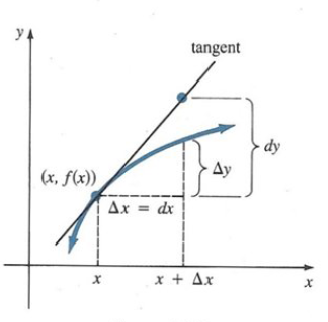
\includegraphics[width=0.4\textwidth]{tan.png}\\[1cm]
  \end{center}
 
\noindent This is also written as 
\begin{equation*}
f(x+\Delta x)=f(x)+\Delta y =f(x)+f'(x)\Delta x.
\end{equation*}

\noindent \textbf{Example:} Approximate $\sqrt{10}$ by differentials.

\noindent \textbf{Solution:} $\sqrt{10}$ is near $\sqrt{9}$, so we will use $f(x)=\sqrt{x}$ with $x=9$ and $\Delta x =10-9=1$. Note that $f'(x)=\dfrac{1}{2\sqrt{x}}$. Therefore
\begin{eqnarray*}
\sqrt{10} &=& f(x+\Delta x)\\
&\approx & f(x)+ f'(x)\Delta x\\
&=& \sqrt{x} +\dfrac{1}{2\sqrt{x}}\Delta x =\sqrt{9} +\dfrac{1}{2\sqrt{9}} (1)\\
&=& \dfrac{19}{6}.
\end{eqnarray*}
\noindent \textbf{Example:} Find an approximate value of $\sqrt[3]{9}$.

\noindent \textbf{Solution:} We set $f(x)=\sqrt[3]{x}$. Suppose to find $f(9)$. Note that $f'(x)=\frac{1}{3}x^{-\frac{2}{3}}$ and hence, $f(8)=2$ and $f'(8)=\frac{1}{12}$, where $x=8$ and $\Delta x =9-8=1$. Therefore, 
\begin{eqnarray*}
\sqrt[3]{9} &=& f(9) \approx 2+\dfrac{1}{12} (1)\\
&=& \dfrac{25}{12}\\
&\approx & 2.0833.
\end{eqnarray*}
 \noindent \textbf{Example:} Find an approximate value for $\tan 46^\circ$.
 
 \noindent \textbf{Solution:} Radial measure $46^\circ =45^\circ +1^\circ$ corresponds to $\dfrac{\pi}{4} +\dfrac{\pi}{180}$ and note that $f(x)=\tan x$, then $f'(x)=\sec ^2 x$ and $f(\frac{\pi}{4})=1, \, f'(\frac{\pi}{4})=2$. Therefore
 \begin{equation*}
 \tan 46^\circ = \tan \left(\dfrac{\pi}{4}+\dfrac{\pi}{180}\right) \approx \tan \frac{\pi}{4} +\sec ^2 \frac{\pi}{4} \left(\dfrac{\pi}{180}\right) = 1+\dfrac{\pi}{90} \approx 1.0349.
 \end{equation*} 
 \section{The Mean Value Theorem}
 Suppose $f(x)$ is continuous on $[a,b]$ and differentiable on $(a,b)$. Then, there exists a $c$ in $(a,b)$ at which the tangent line is parallel to the secant line joining the points $(a,f(a))$ and $(b,f(b))$, i.e., at which $f'(c)=\dfrac{f(b)-f(a)}{b-a}$, 
 
 \noindent \textbf{OR} \\
 
 
\noindent  If $f(x)$ is continuous in $[a,b]$ and differentiable in $(a,b)$, then there exists a point $c$ in $(a,b)$ such that 
 \begin{equation*}
 f'(c)=\dfrac{f(b)-f(a)}{b-a}, \quad a<c<b.
 \end{equation*}
 \begin{center}
 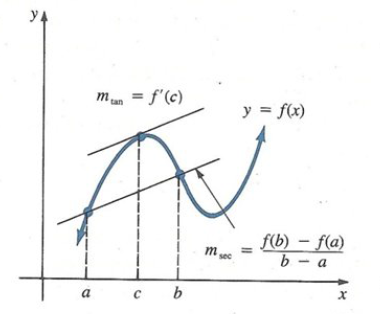
\includegraphics[width=0.4\textwidth]{mean.png}\\[1cm]
  \end{center}
 \noindent The word \textbf{mean} in The Mean Value Theorem refers to the mean (or average) rate of change of $f$ in the interval $[a,b]$.
 
 
\noindent If $f(a)=f(b)=0$, then the theorem says that there exists a $c$ in $(a,b)$ at which $f'(c)=0$. The graphs suggest that there must be at least one point on the graph, that corresponds to a number $c$ in $(a,b)$, at which the tangent is horizontal. This special case of the Mean Value Theorem is called \textbf{Rolle's Theorem} \footnote{Michel Rolle, a French mathematician (1652-1719)}. 
\begin{center}
 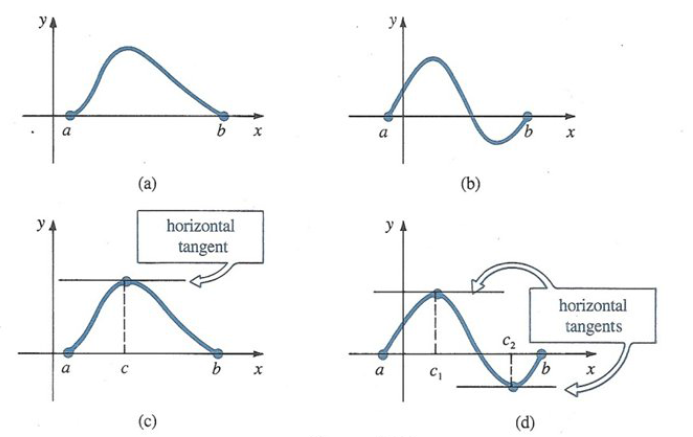
\includegraphics[width=0.6\textwidth]{rolle.png}\\[1cm]
  \end{center}
\noindent \textbf{Example:} Consider $f(x)=\sqrt{x-1}$ on $[2,5]$, $f(x)$ is continuous when $x-1\geq 0$, i.e., $x\geq 1$. In particular, $f(x)$ is continuous on $[2,5]$ and $f'(x)=\dfrac{1}{2\sqrt{x-1}}$, so differentiable when $x>1$. In particular, $f(x)$ is differentiable on $(2,5)$. 
\begin{equation*}
\dfrac{f(b)-f(a)}{b-a} =\dfrac{f(5)-f(2)}{5-2} =\dfrac{\sqrt{5-1}-\sqrt{2-1}}{3}=\dfrac{1}{3}.
\end{equation*} 
The Mean Value Theorem asserts that, for some $c$ in $(2,5), \, f'(c)=\dfrac{1}{3}$. Let us find it.
\begin{eqnarray*}
f'(x) &=&\dfrac{1}{3}\\
\dfrac{1}{2\sqrt{x-1}} &=&\dfrac{1}{3}\\
2\sqrt{x-1} &=& 3\\
4(x-1) &=& 9\\
x-1 &=&\dfrac{9}{4}\\
x &=& \dfrac{13}{4}.
\end{eqnarray*}
Notice that $\dfrac{13}{4}$ is in $(2,5)$, so we may take $c=\dfrac{13}{4}$.

\noindent \textbf{Example:} Show that if $f(x)=\tan x$ on the interval $0\leq x\leq k$ where $k<\dfrac{\pi}{2}$, then $\tan k \geq k$.

\noindent \textbf{Solution:} By the Mean Value Theorem
\begin{equation*}
\dfrac{\tan k -\tan 0}{k-0} =\sec ^2 c,
\end{equation*}
 for some $c\in (0,k)$. But $\sec ^2 c \geq 1$ and $\tan 0 =0$. So 
 \begin{equation*}
 \dfrac{\tan k}{k} \geq 1 \Longrightarrow \tan k \geq k.
 \end{equation*}
 
 \noindent \textbf{Example:} Use The Mean Value Theorem to show that $|\cos a -\cos b|\leq |a-b|$.
 
 \noindent \textbf{Solution:} The function $\cos x$ is continuous and differentiable for all $x$. By the Mean Value Theorem
 \begin{eqnarray*}
 (\cos x)' &=& \dfrac{\cos a -\cos b}{a-b}\\
 |(\cos x)'| &=& \left|\dfrac{\cos a -\cos b}{a-b} \right|,
 \end{eqnarray*}
 but $(\cos x)'=-\sin x$ and $|(\cos x)'|\leq 1$, therefore
 \begin{equation*}
 \dfrac{|\cos a -\cos b|}{|a-b|}\leq 1 \Longrightarrow |\cos a -\cos b|\leq |a-b|.
 \end{equation*}
 
 \noindent \textbf{Example:} Prove that $\dfrac{b-a}{1+b^2}<\tan ^{-1} b -\tan ^{-1} a < \dfrac{b-a}{1+a^2}$ for $a<b$.
 
 \noindent \textbf{Solution:} Let $f(x)=\tan ^{-1} x $. Since $f'(x)=\dfrac{1}{1+x^2}, \,f'(c)=\dfrac{1}{1+c^2} $. By the Mean Value Theorem
 \begin{equation*}
 \dfrac{f(b)-f(a)}{b-a}=\dfrac{\tan ^{-1} b-\tan ^{-1} a}{b-a} =\dfrac{1}{1+c^2}, \quad a<c<b.
 \end{equation*}
 Then, from $a<c<b$, we have 
 \begin{eqnarray*}
 a^2<c^2<b^2 &\Longrightarrow& 1+a^2<1+c^2<1+b^2\\
 \dfrac{1}{1+a^2}>\dfrac{1}{1+c^2}>\dfrac{1}{1+b^2} &\Longrightarrow &  \dfrac{1}{1+b^2}<\dfrac{1}{1+c^2}<\dfrac{1}{1+a^2}\\
 \dfrac{1}{1+b^2}<\dfrac{\tan ^{-1} b -\tan ^{-1} a}{b-a} <\dfrac{1}{1+a^2} &\Longrightarrow & \dfrac{b-a}{1+b^2}<\tan ^{-1} b -\tan ^{-1} a < \dfrac{b-a}{1+a^2}.
 \end{eqnarray*}
 
 \noindent \textbf{Example:} Use the Mean Value Theorem, to prove that if $0<a<b$, then $1-\dfrac{a}{b}<\ln \left(\dfrac{b}{a}\right)<\dfrac{b}{a}-1$. Hence show that $\dfrac{1}{6}<\ln 1.2 < \dfrac{1}{5}$.
 
 \noindent \textbf{Solution:} Let $f(x)=\ln x$ and $f'(x)=\dfrac{1}{x}$. By the Mean Value Theorem, there exists $c\in (a,b)$ such that 
 \begin{equation*}
f'(c)=\dfrac{1}{c}=\dfrac{\ln b -\ln a}{b-a}. 
 \end{equation*}
 Then, from $a<c<b$ we have
 \begin{eqnarray*}
 a<c<b  &\Longrightarrow & \dfrac{1}{b}< \dfrac{1}{c} <\dfrac{1}{a} \\
 \dfrac{1}{b} <\dfrac{\ln b -\ln a}{b-a} <\dfrac{1}{a} &\Longrightarrow & \dfrac{b-a}{b}<\ln b -\ln a < \dfrac{b-a}{a}\\
 &\Longrightarrow & 1-\dfrac{a}{b}<\ln \left(\dfrac{b}{a}\right)<\dfrac{b}{a}-1.
 \end{eqnarray*}
 
\noindent Now, $\ln (1.2)=\ln \left(\dfrac{12}{10}\right)=\ln \left(\dfrac{6}{5} \right)$. Therefore $a=5$ and $b=6$. Substituting in \\$1-\dfrac{a}{b}<\ln \left(\dfrac{b}{a}\right)<\dfrac{b}{a}-1$, we have 
\begin{equation*}
1-\dfrac{5}{6}<\ln \left(\dfrac{6}{5}\right)<\dfrac{6}{5}-1 \Longrightarrow \dfrac{1}{6}<\ln 1.2 < \dfrac{1}{5}.
\end{equation*}
\section{Some Corollaries of The Mean Value Theorem}
\begin{corollary}
If $f'(x)=0$ at all points of the interval $(a,b)$, then $f(x)$ must be a constant in the interval.
\end{corollary}
\begin{proof}
Let $x_1<x_2$ be any two different points in $(a,b)$. By the Mean Value Theorem for\\
 $x_1<x<x_2$, 
\begin{equation*}
\dfrac{f(x_2)-f(x_1)}{x_2-x_1} =f'(x)=0.
\end{equation*} 
Thus $f(x_1)=f(x_2)$. Since $x_1$ and $x_2$ are arbitrarily chosen, the function $f(x)$ has the same value at all points in the interval. Thus, $f(x)$ is constant.
\end{proof}
\begin{corollary}
If $f'(x)>0$ at all points of the interval $(a,b)$, then $f(x)$ is strictly increasing.
\end{corollary}
\begin{proof}
Let $x_1<x_2$ be any two different points in $(a,b)$. By the Mean Value Theorem for\\ $x_1<x<x_2$, 
\begin{equation*}
\dfrac{f(x_2)-f(x_1)}{x_2-x_1} =f'(x)>0.
\end{equation*}
Thus $f(x_2)>f(x_1)$ for $x_2>x_1$ and so $f(x)$ is strictly increasing.
\end{proof}
\section{Indeterminate Forms}
Happens when $\displaystyle \lim _{x\rightarrow a} \dfrac{f(x)}{g(x)}$ tends to  $\dfrac{0}{0}$ or $\dfrac{\infty}{\infty}$ as $x\rightarrow a$. Think of the situation $\displaystyle \lim _{x\rightarrow a} \dfrac{f(x)}{g(x)}\rightarrow \dfrac{0}{0}$ where $f(x)$ and $g(x)$ are differentiable  (and therefore continuous  so $f(a)=\displaystyle \lim _{x\rightarrow a} f(x)=0$ and $g(a)=\displaystyle \lim _{x\rightarrow a}g(x)=0$.), then 
\begin{eqnarray*}
\lim _{x\rightarrow a} \dfrac{f(x)}{g(x)} &=& \lim _{x\rightarrow a} \dfrac{f(x)-f(a)}{g(x)-g(x)}\\
&=& \lim _{x\rightarrow a} \dfrac{\dfrac{f(x)-f(a)}{x-a}}{\dfrac{g(x)-g(a)}{x-a}} \quad \hbox{(provided the denominator is not zero)}\\
&=& \dfrac{\displaystyle \lim _{x\rightarrow a}\dfrac{f(x)-f(a)}{x-a}}{\displaystyle \lim _{x\rightarrow a}\dfrac{g(x)-g(a)}{x-a}}\\
&=& \dfrac{f'(a)}{g'(a)} =\dfrac{\displaystyle \lim _{x\rightarrow a} f'(x)}{\displaystyle \lim _{x\rightarrow a} g'(x)} \quad \hbox{(provided $f'(x)$ and $g'(x)$ are also continuous.)}
\end{eqnarray*}

\noindent \textbf{Example:} 
\begin{equation*}
\lim _{x\rightarrow 2} \dfrac{x^2-4}{x-2} =\lim _{x\rightarrow 2} \dfrac{(x^2-4)'}{(x-2)'}=\lim _{x\rightarrow 2} \dfrac{2x}{1}=2\cdot 2 =4.
\end{equation*}

\begin{theorem}
If $\displaystyle \lim  \dfrac{f(x)}{g(x)}=\lim \dfrac{f'(x)}{g'(x)}$ provided that $\displaystyle \lim \dfrac{f(x)}{g(x)}$ is of the type $\dfrac{0}{0}$ or $\dfrac{\infty}{\infty}$, this is called \textbf{L'H$\hat{o}$pital's Rule}: if either $\displaystyle \lim \dfrac{f(x) }{g(x)}=\dfrac{0}{0}$ or $\dfrac{\infty}{\infty}$.
\end{theorem}

\noindent \textbf{Examples:} (a)\, $\displaystyle \lim _{x\rightarrow 0}\dfrac{\sin 2x}{\sin 5x}=\lim _{x\rightarrow 0}\dfrac{2\cos 2x}{5\cos 5x}=\dfrac{2\cdot 1}{5\cdot 1}=\dfrac{2}{5}$. \\
(b)\, $\displaystyle \lim _{x\rightarrow \infty} \dfrac{e^{3x}}{x}=\lim _{x\rightarrow \infty} \dfrac{3e^{3x}}{1}=\infty$.\\
(c)\, $\displaystyle \lim _{x\rightarrow 0} \dfrac{e^x-1}{x^3}=\lim _{x \rightarrow 0} \dfrac{e^x}{3x^2}=\infty$.

\noindent \textbf{The form $\infty -\infty$.} A given limit that is not immediately $\dfrac{0}{0}$ or $\dfrac{\infty}{\infty}$ can be converted to one of these forms by combination of algebra and a little cleverness. 

\noindent \textbf{Example:}  Evaluate $\displaystyle \lim _{x\rightarrow 0} \left[\dfrac{1+3x}{\sin x}-\dfrac{1}{x}\right]$.

\noindent \textbf{Solution:} We note $\dfrac{1+3x}{\sin x}\rightarrow \infty$ and $\dfrac{1}{x}\rightarrow \infty$. However, after writing the difference as a single fraction, we recognize the form $\dfrac{0}{0}$.
\begin{eqnarray*}
\lim _{x\rightarrow 0} \left[\dfrac{1+3x}{\sin x}-\dfrac{1}{x}\right] &=& \lim _{x\rightarrow 0} \dfrac{3x^2+x-\sin x}{x\sin x}\\
&=& \lim _{x\rightarrow 0} \dfrac{6x+1-\cos x}{x\cos x +\sin x}\\
&=& \lim _{x\rightarrow 0} \dfrac{6+\sin x}{-x\sin x +2\cos x } \\
&=& \dfrac{6+0}{0+2} =3.
\end{eqnarray*}

\noindent \textbf{The form $0\cdot \infty$.} By suitable manipulation, L'H$\hat{o}$pital's Rule can sometimes be applied to the limit form $0\cdot \infty$.

\noindent \textbf{Example:} Evaluate $\displaystyle \lim _{x\rightarrow \infty} x\sin \left(\dfrac{1}{x}\right)$.

\noindent \textbf{Solution:} Write the given expression as 
\begin{equation*}
\lim _{x\rightarrow \infty} \dfrac{\sin \left(\dfrac{1}{x}\right)}{\dfrac{1}{x} }
\end{equation*}
and recognize that we have the form $\dfrac{0}{0}$. Hence, 
\begin{eqnarray*}
\lim _{x\rightarrow \infty} x\sin \left(\dfrac{1}{x}\right) &=& \lim _{x\rightarrow \infty}\dfrac{(-x^{-2}\cos \frac{1}{x})}{(-x^{-2})}\\
&=& \lim _{x\rightarrow \infty} \cos \frac{1}{x} =1.
\end{eqnarray*}

\noindent \textbf{The form $0^0, \, \infty ^0, \, 1^\infty$.} Suppose $y=f(x)^{g(x)}$ tends towards   $0^0, \, \infty ^0, \, 1^\infty$ as $x\rightarrow a$ or $x\rightarrow \infty$. By taking the natural logarithm of $y$ ;
\begin{equation*}
\ln y=\ln f(x)^{g(x)} =g(x)\ln f(x)
\end{equation*}
and we see 
\begin{equation*}
\lim _{x\rightarrow a} \ln y =\lim _{x\rightarrow a} g(x)\ln f(x)
\end{equation*}
is of the form $0\cdot \infty$. If it is assumed that $\displaystyle \lim _{x\rightarrow a} \ln y =\ln (\lim _{x\rightarrow a} y)=L$, then $\displaystyle \lim _{x\rightarrow a}= e^L$ or 
\begin{equation*}
\lim _{x\rightarrow a} f(x)^{g(x)} =e^L.
\end{equation*}

\noindent \textbf{Example:} Evaluate $\displaystyle \lim _{x\rightarrow 0^+} x^{\frac{1}{\ln x}}$.

\noindent \textbf{Solution:} The form is $0^0$. Now, if we set $y=x^{\frac{1}{\ln x}}$, then 
\begin{equation*}
\ln y= \dfrac{1}{\ln x} \ln x =1.
\end{equation*}
Notice we do not need L'H$\hat{o}$pital's Rule in this case since 
\begin{equation*}
\lim _{x\rightarrow 0^+} \ln y =1.
\end{equation*}
Hence, $\displaystyle \lim _{x\rightarrow 0^+}y =e^1$ or equivalently $\displaystyle \lim _{x\rightarrow 0^+}x^{\frac{1}{\ln x}}=e$.

\noindent \textbf{Example:} Evaluate $\displaystyle \lim _{x\rightarrow 0} (1+x)^{\frac{1}{x}}$.

\noindent \textbf{Solution:} The limit form is of the form $1^\infty$. If $y=(1+x)^{\frac{1}{x}}$, then 
\begin{equation*}
\ln y =\frac{1}{x}\ln (1+x).
\end{equation*}
Now, $\displaystyle \lim _{x\rightarrow 0} \dfrac{\ln (1+x)}{x}$ has the form $\dfrac{0}{0}$ and so 
\begin{eqnarray*}
\lim _{x\rightarrow 0}\dfrac{\ln (1+x)}{x} &=& \lim _{x\rightarrow 0} \dfrac{\frac{1}{1+x}}{1}\\
&=& \lim _{x\rightarrow 0}  \dfrac{1}{1+x} =1.
\end{eqnarray*}
Thus, 
\begin{equation*}
\lim _{x\rightarrow 0} (1+x)^{\frac{1}{x}} =e.
\end{equation*}

\noindent \textbf{Example:} Evaluate $\displaystyle \lim _{x\rightarrow \infty} \left(1-\dfrac{3}{x}\right)^{2x}$.

\noindent \textbf{Solution:} The limit form is $1^\infty$. If $y=\left(1-\dfrac{3}{x}\right)^{2x}$ then $\ln y =2x \ln \left(1-\dfrac{3}{x}\right)$. Observe that the form $\displaystyle \lim _{x\rightarrow \infty}2x \ln \left(1-\dfrac{3}{x}\right)$ is $\infty \cdot 0$, whereas the form of $\displaystyle \lim _{x\rightarrow \infty} \dfrac{2\ln (1-\frac{3}{x})}{\frac{1}{x}}$ is $\dfrac{0}{0}$. Therefore, 
\begin{eqnarray*}
\lim _{x\rightarrow \infty} \dfrac{2\ln (1-\frac{3}{x})}{\frac{1}{x}} &=& \lim _{x\rightarrow \infty} 2\dfrac{\dfrac{\frac{3}{x^2}}{(1-\frac{3}{x})}}{-\frac{1}{x^2}} \\
&=& \lim _{x\rightarrow \infty} \dfrac{-6}{(1-\frac{3}{x})} =-6.
\end{eqnarray*}
Finally, we conclude that 
\begin{equation*}
\lim _{x\rightarrow \infty} \left( 1-\dfrac{3}{x}\right)^{2x}=e^{-6}.
\end{equation*}
\section{Extrema of Functions}
Suppose a function $f$ is defined on an interval $I$. The \textbf{maximum} and \textbf{minimum} values of $f$ on $I$ (if there are any) are said to be \textbf{extrema} of the function. 
\begin{definition}
\begin{itemize}
\item[(i)] A number $f(c_1)$ is an \textbf{absolute maximum} of a function $f$ if $f(x)\leq f(c_1)$ for every $x$ in the domain of $f$.
\item[(ii)] A number $f(c_1)$ is an \textbf{absolute minimum} of a function $f$ if $f(x)\geq f(c_1)$ for every $x$ in the domain of $f$.
\end{itemize}
\end{definition}
\begin{center}
 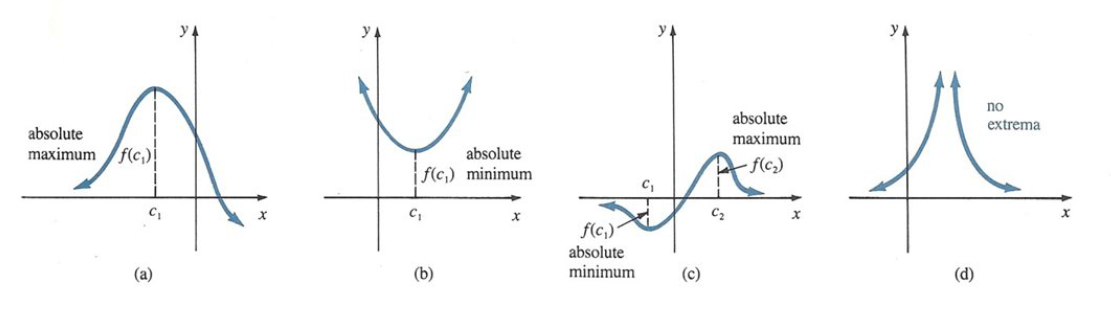
\includegraphics[width=0.8\textwidth]{good.png}\\[1cm]
  \end{center}
\noindent \textbf{Example:} The function $f(x)=x^2$ has the absolute minimum $f(0)=0$ but has no absolute maximum.

\noindent \textbf{Example:} $f(x)=\dfrac{1}{x}$ has neither an absolute maximum nor an absolute minimum.

\noindent The interval on which a function is defined is very important in the consideration of extrema. 

\noindent \textbf{Example:} $f(x)=x^2$ defined only on the closed interval $[1,2]$, has the absolute maximum $f(2)=4$ and the absolute minimum $f(1)=1$. On the other hand, if $f(x)=x^2$ is defined on the open interval $(1,2)$, then $f$ has no absolute extrema. In this case, $f(1)$ and $f(2)$ are not defined.

\begin{theorem}[Extreme Value Theorem]
A function $f$ continuous on $[a,b]$ always has an absolute maximum and an absolute minimum on the interval.
\end{theorem}
\begin{definition}
\begin{itemize}
\item[(i)] A number $f(c_1)$ is a \textbf{relative maximum} of a function $f$ if $f(x)\leq f(c_1)$ for every $x$ in some open interval that contains $c_1$.
\item[(ii)] A number $f(c_1)$ is a \textbf{relative minimum} of a function $f$ if $f(x)\geq f(c_1)$ for every $x$ in some open interval that contains $c_1$.
\end{itemize}
\end{definition}

\begin{definition}
A \textbf{critical value} of a function $f$ is a number $c$ in its domain for which $f'(c)=0$ or $f'(c)$ does not exist.
\end{definition}
\noindent \textbf{Example:} Find the critical values of $f(x)=x^3-15x+6$.

\noindent \textbf{Solution:} 
\begin{equation*}
f'(x)=3x^2-15.
\end{equation*}
The critical values are those numbers for which $f'(x)=0$, namely $\pm \sqrt{5}$.

\noindent \textbf{Example:} Find the critical value of $f(x)=(x+4)^{\frac{2}{3}}$.

\noindent \textbf{Solution:} By power rule for functions,  
\begin{equation*}
f'(x)=\dfrac{2}{3}(x+4)^{-\frac{1}{3}}=\dfrac{2}{3(x+4)^{\frac{1}{3}}}.
\end{equation*}
In this instance we see that $f'(x)$ does not exist when $x=-4$. Since $-4$ is in the domain of $f$, we conclude it is a critical value.

\begin{theorem}
If a function $f$ has a relative extremum at a number $c$, then $c$ is a critical value.
\end{theorem}
\section{Tutorial Questions}
\begin{enumerate}
\item Evaluate each of the following limits using L'hopital's rule.\\
(i)\, $\displaystyle \lim _{x\rightarrow 0}\dfrac{\sin x}{x}$ \quad (ii)\, $\displaystyle \lim _{x\rightarrow 0}\dfrac{\sin x}{e^x-e^{-x}}$ \quad (iii)\, $\displaystyle \lim _{x\rightarrow \infty}\dfrac{\ln x}{e^x}$ \quad (iv)\, $\displaystyle \lim _{x\rightarrow \infty}\dfrac{6x^2-5x+7}{4x^2-2x}$\\
(v)\, $\displaystyle \lim _{x\rightarrow \infty}\dfrac{e^{3x}}{x^2}$ \quad (vi)\, $\displaystyle \lim _{x\rightarrow \infty}\dfrac{x^4}{e^{2x}}$ \quad (vii)\, $\displaystyle \lim _{t\rightarrow {\frac{\pi}{4}}^+}\dfrac{\tan t}{\tan 3t}$ \quad (viii)\, $\displaystyle \lim _{x\rightarrow {1}^+}\dfrac{\ln x}{\sqrt{x-1}}$\\
(ix)\, $\displaystyle \lim _{x\rightarrow 0}\left[\dfrac{1+3x}{\sin x}-\dfrac{1}{x}\right]$ \quad (x)\, $\displaystyle \lim _{x\rightarrow \infty}x\sin \left(\frac{1}{x}\right)$ \quad (xi)\, $\displaystyle \lim _{x\rightarrow 0} x^{\frac{1}{\ln x}}$ \quad (xii)\, $\displaystyle \lim _{x\rightarrow 0}(1+x)^{\frac{1}{x}}$\\
(xiii)\, $\displaystyle \lim _{x\rightarrow \infty}\left(1-\frac{3}{x}\right)^{2x}$ \quad (xiv)\, $\displaystyle \lim _{x\rightarrow 0^+}x^x$ \quad (xv)\, $\displaystyle \lim _{x\rightarrow \infty}x(e^{\frac{1}{x}}-1)$ \quad (xvi)\, $\displaystyle \lim _{x\rightarrow 0}\left(\dfrac{1}{x}-\dfrac{1}{\sin x}\right)$.
\item Evaluate each of the following limits using L'Hopital's rule.\\
(i)\, $\displaystyle \lim _{x\rightarrow \infty}(2+e^x)^{e^{-x}}$ \quad (ii)\, $\displaystyle \lim _{x\rightarrow 0^-}(1-e^x)^{x^2}$ \quad (iii)\, $\displaystyle \lim _{x\rightarrow \infty}x^2e^{-x}$ \quad (iv)\, $\displaystyle \lim _{x\rightarrow \infty} (x+e^x)^{\frac{2}{x}}$\\
(v)\, $\displaystyle \lim _{x\rightarrow 0}x\ln (\sin x)$ \quad (vi)\, $\displaystyle \lim _{x\rightarrow 0}x^{\ln ^2 x}$ \quad (vii)\, $\displaystyle \lim _{x\rightarrow 0}(1+5\sin x)^{\cot x}$ \quad (viii)\, $\displaystyle \lim _{x\rightarrow \infty}\left(\dfrac{3x}{3x+1}\right)^x$\\
(ix)\, $\displaystyle \lim _{x\rightarrow 0}x^{(1-\cos x)}$ \quad (x)\, $\displaystyle \lim _{t\rightarrow \infty}\left(1+\frac{3}{t}\right)^t$ \quad (xi)\, $\displaystyle \lim _{x\rightarrow 0}\left(\dfrac{1}{e^x-1}-\dfrac{1}{x}\right)$ \quad (xii)\, $\displaystyle \lim _{x\rightarrow 0}\dfrac{\tan x}{2x}$\\
(xiii)\, $\displaystyle \lim _{x\rightarrow 0^+}(1+x)^{\frac{1}{x^2}}$ \quad (xiv)\, $\displaystyle \lim _{x\rightarrow {\frac{\pi}{2}}^+}(\sin ^2 x)^{\tan x}$ \quad (xv)\, $\displaystyle \lim _{\theta\rightarrow 0}\theta \csc 4\theta$ \quad (xvi)\, $\displaystyle \lim _{x\rightarrow 0^+}x\ln x$.
\item Evaluate each of the following using L'hopital's rule.\\
(i)\, $\displaystyle \lim _{r\rightarrow 0}\dfrac{r-\cos r}{r-\sin r}$ \quad (ii)\, $\displaystyle \lim _{x\rightarrow -\infty}\dfrac{1+e^{-2x}}{1-e^{-2x}}$ \quad (iii)\, $\displaystyle \lim _{x\rightarrow 0}\dfrac{e^x-x-1}{2x^2}$ \quad 
(iv)\, $\displaystyle \lim _{x\rightarrow 0}\dfrac{x-\tan ^{-1}x}{x-\sin ^{-1} x}$\\ (v)\, $\displaystyle \lim _{x\rightarrow 0^+}(\cos x)^{\frac{1}{x^2}}$ \quad (vi)\, $\displaystyle \lim _{x\rightarrow \infty}\left(1+\frac{a}{x}\right)^x$ \quad (vii)\, $\displaystyle \lim _{x\rightarrow \infty}x^{\frac{1}{x}}$ \quad (viii)\, $\displaystyle \lim _{x\rightarrow \frac{\pi}{4}}(\tan x)^{\tan x}$\\
(ix)\, $\displaystyle \lim _{x\rightarrow 0}(x^2)^x$ \quad (x)\, $\displaystyle \lim _{x\rightarrow 0}x^3\ln x$ \quad (xi)\, $\displaystyle \lim _{x\rightarrow 0}\dfrac{3^x-2^x}{x}$ \quad (xii)\, $\displaystyle \lim _{x\rightarrow 1^+}(\ln x)^{\ln x}$\\
(xiii)\, $\displaystyle \lim _{x\rightarrow 0}x^{\sin x}$ \quad (xiv)\, $\displaystyle \lim _{x\rightarrow \infty}(1+2x)^{\frac{1}{3x}}$ \quad (xv)\, $\displaystyle \lim _{x\rightarrow 0}\left(\dfrac{e^x\sec x}{x}-\dfrac{\sin x}{x^2}\right)$ \quad (xvi)\, $\displaystyle \lim _{x\rightarrow \infty}\dfrac{(x^2+3x+3)^{x+1}}{(x+1)^{2x+1}(x+2)}$.

\end{enumerate}
\section{Graphing and the First Derivative}
Knowing that a function does, or does not, possess relative extrema is a great aid in drawing its graph. 
\begin{theorem}
Let $f$ be continuous on $[a,b]$ and differentiable on $(a,b)$, except possibly at the critical value $c$.
\begin{itemize}
\item[(i)] If $f'(x)>0$ for $a<x<c$ and $f'(x)<0$ for $c<x<b$, then $f(c)$ is a \textbf{relative maximum}.
\item[(ii)]  If $f'(x)<0$ for $a<x<c$ and $f'(x)>0$ for $c<x<b$, then $f(c)$ is a \textbf{relative minimum}.
\item[(iii)] If $f'(x)$ has the same algebraic sign on $a<x<c$ and $c<x<b$, then $f(c)$ is not an extremum.
\end{itemize}
\end{theorem}
\begin{center}
 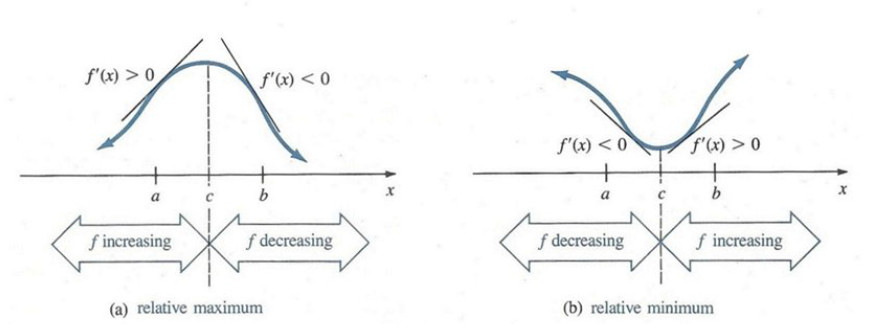
\includegraphics[width=0.8\textwidth]{min.png}\\[1cm]
  \end{center}
\noindent \textbf{Example:} For each of the following functions, find all the critical points and classify each as a relative maximum, relative minimum or neither. (a)\, $f(x)=3x^{\frac{5}{3}}-15x^{\frac{2}{3}}$ and (b)\, $f(x)=x^3-3x^2+3x-1$.

\noindent \textbf{Solution:} (a)\,\underline{Critical points:}
\begin{eqnarray*}
f'(x) &=& 5x^{\frac{2}{3}}-10x^{-\frac{1}{3}}\\
&=& 5x^{-\frac{1}{3}}(x-2)\\
&=& \dfrac{5(x-2)}{x^{\frac{1}{3}}},
\end{eqnarray*}
which is zero when $x=2$ and undefined when $x=0$. Therefore $x=0$ is a relative maximum and $x=2$ is a relative minimum.

\noindent (b)\, \underline{Critical points:}
\begin{eqnarray*}
f'(x) &=& 3x^2-6x+3 \\
&=& 3(x^2-2x+1)\\
&=& 3(x-1)^2, 
\end{eqnarray*}
which is defined everywhere and zero when $x=1$. Therefore $x=1$ is neither.

\noindent Sometimes there is an easier way to test a critical point. Our goal is to relate the concept of the concavity of a graph with the second derivative of a function. Often a shape that is concave upwards is said to ``hold water'' whereas a shape that is concave downwards ``spills water''.
\begin{definition}
Let $f$ be differentiable on $(a,b)$.
\begin{itemize}
\item[(i)] If $f'$ is an increasing function on $(a,b)$, then the graph of $f$ is \textbf{concave upwards} on the interval.
\item[(ii)]  If $f'$ is a decreasing function on $(a,b)$, then the graph of $f$ is \textbf{concave downwards} on the interval
\end{itemize}
\end{definition}
\begin{center}
 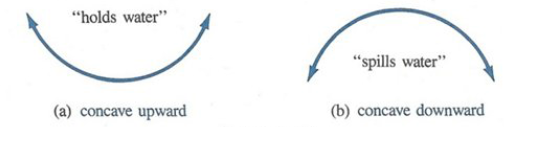
\includegraphics[width=0.5\textwidth]{great.png}\\[1cm]
  \end{center}
\begin{theorem}[Test for Concavity] Let $f$ be a function for which $f''$ exists on $(a,b)$.
\begin{itemize}
\item[(i)] If $f''(x)>0$ for all $x$ in $(a,b)$, then the graph is concave upward on $(a,b)$.
\item[(ii)] If $f''(x)<0$ for all $x$ in $(a,b)$, then the graph is concave downward on $(a,b)$.
\end{itemize}
\end{theorem}
\begin{center}
 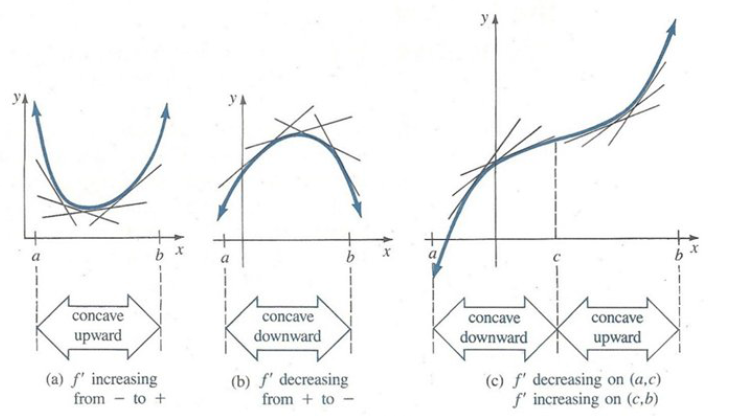
\includegraphics[width=0.6\textwidth]{turn.png}\\[1cm]
  \end{center}
\noindent \textbf{Example:} Determine the intervals on which the graph of $f(x)=-x^3+\frac{9}{2}x^2$ is concave upward and the intervals for which the graph is concave downward.

\noindent \textbf{Solution:} From 
\begin{eqnarray*}
f'(x) &=& -3x^2+9x\\
f''(x) &=& -6x+9 =6\left(-x+\frac{3}{2}\right),
\end{eqnarray*}
we see that $f''(x)>0$ when $6\left(-x+\frac{3}{2}\right)>0 $ or $x<\frac{3}{2}$ and that $f''(x)<0$ when $6\left(-x+\frac{3}{2}\right)<0$ or $x>\frac{3}{2}$. It follows that the graph of $f$ is concave upward on $(-\infty , \frac{3}{2})$ and concave downward on $(\frac{3}{2}, \infty)$.

\subsection{Point of Inflection}
\begin{definition}
Let $f$ be continuous at $c$. A point $(c, f(c))$ is a \textbf{point of inflection} if there exists  an open interval $(a,b)$ that contains $c$ such that the graph of $f$ is either 
\begin{itemize}
\item[(i)] concave upward on $(a,c)$ and concave downward on $(c,b)$ or 
\item[(ii)] concave downward on $(a,c)$ and concave upward on $(c,b)$.
\end{itemize}
\end{definition}
\noindent As a consequence, we observe that \textit{a point of inflection $(c,f(c))$ occurs at a number $c$ for which $f''(c)=0$ or $f''(c)$ does not exist}.

\noindent \textbf{Example:} Find any points of inflection of $f(x)=-x^3+x^2$.

\noindent \textbf{Solution:} The first and second derivatives of $f$ are, respectively, 
\begin{equation*}
f'(x)=-3x^2+2x \quad \hbox{and}~~ f''(x)=-6x+2.
\end{equation*}
Since $f''(x)=0$ at $\frac{1}{3}$, the point $(\frac{1}{3}, \frac{2}{27})$ is the only possible point of inflection. Now, 
\begin{eqnarray*}
f''(x) &=& 6\left(-x+\frac{1}{3}\right)>0\quad  \hbox{for}~~ x<\frac{1}{3}\\
f''(x) &=& 6\left(-x+\frac{1}{3}\right)<0\quad  \hbox{for}~~ x>\frac{1}{3}, 
\end{eqnarray*}
implies that the graph of $f$ is concave upward on $(-\infty , \frac{1}{3})$ and concave downward on $(\frac{1}{3}, \infty)$. Thus $(\frac{1}{3}, f(\frac{1}{3}))$ or $(\frac{1}{3}, \frac{2}{27})$ is a point of inflection.

\noindent \textbf{Second Derivative Test.} If $c$ is a critical value of $y=f(x)$ and, say, $f''(c)>0$, then the graph of $f$ is concave upward on some interval $(a,b)$ that contains $c$.  Necessarily then, $f(c)$ is a relative minimum. Similarly, $f''(c)<0$ at a critical value $c$ implies $f(c)$ is a relative maximum.
\begin{theorem}[Second Derivative Test for Relative Extrema] Let $f$ be a function for which $f''$ exists on an interval $(a,b)$ that contains the critical number $c$. 
\begin{itemize}
\item[(i)] If $f''(c)>0$, then $f(c)$ is a relative minimum.
\item[(ii)] If $f''(c)<0$, then $f(c)$ is a relative maximum.
\end{itemize} 
\end{theorem}
\begin{center}
 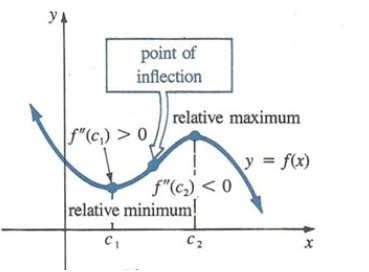
\includegraphics[width=0.3\textwidth]{point.png}\\[1cm]
  \end{center}
\noindent However, if $f''(c)=0$ then nothing can be concluded about the nature of the critical point.

\noindent \textbf{Example:} for each of the following functions, find all of the critical points and classify each as relative maximum, relative minimum or neither. (a)\, $f(x)=x^3-3x+2$ \quad (b)\, $f(x)=\frac{1}{2}x-\sin x$ on $0<x<2\pi$.

\noindent \textbf{Solution:} (a)\, 
\begin{eqnarray*}
f'(x) &=& 3x^2-3 \\
&=& 3(x^2-1) =3(x-1)(x+1),
\end{eqnarray*}
which is defined everywhere and zero at $x=1$ and $x=-1$. Computing $f''(x)=6x$, then 
\begin{eqnarray*}
f''(-1) &=& -6<0 \Rightarrow \hbox{relative maximum at}~~x=-1.\\
f''(1) &=& 6>0 \Rightarrow \hbox{relative minimum at}~~ x=1.
\end{eqnarray*}

\noindent (b)\, $f'(x)=\frac{1}{2}-\cos x$ which is defined everywhere and zero when $\cos x =\frac{1}{2}\Rightarrow x=\frac{\pi}{3}, \frac{5\pi}{3}$. Computing $f''(x)=\sin x$, then 
\begin{eqnarray*}
f''\left(\frac{\pi}{3}\right) &=& \sin \frac{\pi}{3} =\frac{\sqrt{3}}{2} >0 \Rightarrow \hbox{relative minimum at}~~x=\frac{\pi}{3}.\\
f''\left(\frac{5\pi}{3}\right) &=& \sin \frac{5\pi}{3} =-\frac{\sqrt{3}}{2} <0 \Rightarrow \hbox{relative maximum at}~~x= \frac{5\pi}{3}.
\end{eqnarray*}

\section{Sketching the graph of $y=f(x)$}
\section{Tutorial Questions}
\begin{enumerate}
\item Use differentials to compute approximate value of \\
(i)\, $\sqrt[3]{25}$ \quad (ii)\, $\sin 31^\circ$ \quad (iii)\, $\ln (1.12)$ \quad (iv)\, $\sqrt[5]{36}$ \quad (v)\, $\sqrt[5]{31}$ \quad (vi)\, $\cos 62^\circ$ \\
 (vii)\, $\sin 48^\circ$ \quad (viii)\, $(1005)^{\frac{1}{3}}$ \quad (ix)\, $\tan 31^\circ$ \quad (x)\, $\ln (1.2)$ \quad (xi)\, $\sqrt{26}$ \quad (xii)\, $\tan ^{-1}(1.1)$ \\ (xiii)\, $(1.1)^2+6(1.1)^2$ \quad (xiv)\, $\sin 1^\circ$ \quad (xv)\, $\dfrac{1}{\sqrt{96}}$.
 \item Verify Rolle's Theorem for $f(x)=x^2(1-x)^2, \quad 0\leq x\leq 1$.
 \item Find the value of $c$ in Rolle's Theorem when $f(x)=(x-a)^m(x-b)^n$ where $m$ and $n$ are positive integers.
 \item If $f'(x)\leq 0$ at all points of $(a,b)$, prove that $f(x)$ is monotonic decreasing in $(a,b)$. Under what conditions is $f(x)$ strictly decreasing in $(a,b)$?
 \item Use the mean value theorem to show that $\sin x \leq x$ and $\tan x\geq x$. Hence show that $\dfrac{\sin x}{x}$ is strictly decreasing on $(0,\frac{\pi}{2})$.
 \item Suppose $f$ and $g$ are continuous on $[a,b]$, differentiable on $(a,b)$ and $f'(x)=g'(x)$ for all $x\in (a,b)$. Show that $f(x)=g(x)+c$, where $c$ is a constant.
 \item Use the mean value theorem, to prove that, if $0<a<b$, then $(1-\frac{a}{b})<\ln(\frac{b}{a})<(\frac{b}{a}-1)$. Hence show that $\frac{1}{6}<\ln (1.2)<\frac{1}{5}$.
 \item Show that if $0<a<b$, then $\dfrac{b-a}{\sqrt{1-a^2}}<\sin ^{-1} (b)-\sin ^{-1}(a)<\dfrac{b-a}{\sqrt{1-b^2}}$. Hence show that $\left(\dfrac{\pi}{6}+\dfrac{\sqrt{3}}{15}\right)<\sin ^{-1}(0.6)<\left(\dfrac{\pi}{6}+\dfrac{1}{8}\right)$.
 \item Use the Mean Value Theorem to prove the following inequalities
 \begin{itemize}
 \item[(i)] $\ln (1+x) < x$ if $x>0$.
 \item[(ii)] $\sqrt{1+x} <1+\frac{1}{2}x$ if $x>0$.
 \item[(iii)] $\dfrac{x-1}{x}<\ln x <x-1$ for $x>1$.
 \end{itemize}
\item Find the relative extrema of the given functions.\\
(i)\, $f(x)=2x^3+3x^2-36x$ \quad (ii)\, $f(x)=x^5-\frac{5}{3}x^3+2$ \quad (iii)\, $4x-6x^{\frac{2}{3}}+2$ \\ (iv)\, $f(x)=\dfrac{x^2-2x+2}{x-1}$.
\item Find the relative extrema and the points of inflection of the following functions.\\
(i)\, $f(x)=x^4+8x^3+18x^2$ \quad (ii)\, $f(x)=x^6-3x^4+5$ \quad (iii)\, $f(x)=10-(x-3)^{\frac{1}{3}}$ \\
(iv)\, $f(x)=x(x-1)^{\frac{5}{2}}$.
\item Sketch the graphs of the following functions.\\
(i)\, $f(x)=2x^2-5x-3$ \quad (ii)\, $f(x)=\dfrac{x+1}{(x-2)(3x+5)}$ \quad (iii)\, $f(x)=x^4$ \quad (iv)\, $f(x)=x^9$\\
(v)\, $f(x)=\dfrac{2x-1}{(x+2)(x-3)}$ \quad (vi)\, $f(x)=\dfrac{x+1}{x-1}$ \quad (vii)\, $f(x)=\left(\dfrac{x+1}{x-1}\right)^2$.
\end{enumerate}

\chapter{Integration}
\begin{center}
	\small{\parbox{18cm}{
		\begin{raggedright}
		{\small
		\textit{If it's your job to eat a frog, it's best to do it first thing in the morning. And If it's your job to eat two frogs, it's best to eat the biggest one first.}
 }
 
				\vspace{.5cm}\hfill{---Mark Twain}
		\end{raggedright}
	}
} 
\end{center}
\section{Anti-derivatives}
In this chapter we shall see that an equally important problem is :
\begin{equation*}
Given~ a~ function~ f,~ find~ a~ function~ whose~ derivative~ is~ the~ same~ as~ f.
\end{equation*}
That is, for a given function $f$, we wish to find another function $F$ for which $F'(x)=f(x)$ for all $x$ on some interval.
\begin{definition}
A function $F$ is said to be an \textbf{anti-derivative} of a function $f$ if $F'(x)=f(x)$ on some interval.
\end{definition}

\noindent \textbf{Example:} An anti-derivative of $f(x)=2x$ is $F(x)=x^2$ since $F'(x)=2x$.

\noindent There is always more than one anti-derivative of a function. For instance, in the foregoing example, $F_1(x)=x^2-1$ and $F_2(x)=x^2+10$ are also anti-derivatives of $f(x)=2x$ since $F_1'(x)=F_2'(x)=f(x)$. Indeed, if $F$ is an anti-derivative of a function $f$, then so is $G(x)=F(x)+C$, for any constant $C$. This is a consequence of the fact that 
\begin{equation*}
G'(x)=\dfrac{d}{dx}(F(x)+C)=F'(x)+0=F'(x)=f(x).
\end{equation*}
Thus, $F(x)+C$ stands for a \textbf{set of functions} of which each member has a derivative equal to $f(x)$.
\begin{theorem}
If $G'(x)=F'(x)$ for all $x$ in some interval $[a,b]$, then 
\begin{equation*}
G(x)=F(x)+C
\end{equation*}
for all $x$ in the interval.
\end{theorem}

\noindent \textbf{Examples:} (a)\, The anti-derivative of $f(x)=2x$ is $G(x)=x^2+C$.\\
(b)\, The anti-derivative of $f(x)=2x+5$ is $G(x)=x^2+5x+C$ since $G'(x)=2x+5$.

\section{Indefinite Integral }
For convenience let's introduce a notation for an anti-derivative of a function. If $F'(x)=f(x)$, we shall represent the most general anti-derivative of $f$ by 
\begin{equation*}
\int f(x) dx =F(x) +C.
\end{equation*}
The symbol $\displaystyle \int$ is called an \textbf{integral sign}, and the notation $\displaystyle \int f(x)$ is called the \textbf{indefinite integral} of $f(x)$ with respect to $x$. The function $f(x)$ is called the \textbf{integrand}. The process of finding an anti-derivative is called \textbf{anti-differentiation} or \textbf{integration}. The number $C$ is called a \textbf{constant of integration}. Just as $\dfrac{d}{dx} ()$ denotes differentiation with respect to $x$, the symbol $\displaystyle \int ()dx$ denotes integration with respect to $x$.

\section{The Indefinite Integral of a Power}
When differentiating the power $x^n$, we multiply by the exponent $n$ and decrease the exponent by $1$. To find an anti-derivative of $x^n$, the reverse of the differentiation rule would be : \textit{Increase the exponent by $1$ and divide by the new exponent $n+1$}.

\noindent If $n$ is a rational number, then for $n\neq -1$
\begin{equation*}
\int x^n dx =\dfrac{x^{n+1}}{n+1}+C.
\end{equation*}
\begin{proof}
Notice that 
\begin{equation*}
\dfrac{d}{dx}\left(\dfrac{x^{n+1}}{n+1}+C\right) =(n+1)\dfrac{x^{(n+1)-1}}{n+1}+0 =x^n.
\end{equation*}
\end{proof}
\noindent \textbf{Example:} Evaluate (a)\, $\displaystyle \int x^6\, dx$ \quad (b)\, $\displaystyle \int \dfrac{1}{x^5}\,  dx$.

\noindent \textbf{Solution:} \\
(a)\, $\displaystyle \int x^6 \, dx =\dfrac{x^7}{7} +C$.\\
(b)\, By writing $\dfrac{1}{x^5}$ as $x^{-5}$, we have $\displaystyle \int x^{-5}\, dx=\dfrac{x^{-4}}{-4}+C =-\dfrac{1}{4x^4}+C$.

\noindent \textbf{Example:} Evaluate $\displaystyle \int \sqrt{x}\,  dx$.

\noindent \textbf{Solution:} We first write $\displaystyle \int \sqrt{x}\, dx =\int x^{\frac{1}{2}}dx$ and therefore 
\begin{equation*}
\int x^{\frac{1}{2}}dx =\dfrac{x^{\frac{3}{2}}}{\frac{3}{2}} +C=\frac{2}{3}x^{\frac{3}{2}} +C.
\end{equation*}

\noindent The following property of indefinite integrals is an immediate consequence of the fact that the derivative of a sum is the sum of derivatives.

\begin{theorem}
If $F'(x)=f(x)$ and $G'(x)=g(x)$, then 
\begin{equation*}
\int [f(x) \pm g(x)]dx=\int f(x)dx \pm \int g(x)dx =F(x) \pm G(x) +C.
\end{equation*}
\end{theorem}
\noindent \textbf{Example:} Evaluate $\displaystyle \int (x^{-\frac{1}{2}}+x^4)dx$.

\noindent \textbf{Solution:} We can write 
\begin{equation*}
\int (x^{-\frac{1}{2}}+x^4)dx =\int x^{-\frac{1}{2}}dx +\int x^4 dx =\frac{x^{\frac{1}{2}}}{\frac{1}{2}}+\frac{x^5}{5}+C=2x^{\frac{1}{2}}+\frac{x^5}{5}+C.
\end{equation*} 
\begin{theorem}
If $F'(x)=f(x)$, then 
\begin{equation*}
\int kf(x)dx=k\int f(x)dx
\end{equation*}
for any constant $k$.
\end{theorem}

\noindent The anti-derivative, or indefinite integral, of any finite sum can be obtained by integrating each term.

\noindent \textbf{Example:} Evaluate $\displaystyle \int \left(4x-2x^{-\frac{1}{3}}+\frac{5}{x^2} \right)dx$.

\noindent \textbf{Solution:} It follows that 
\begin{eqnarray*}
\int \left(4x-2x^{-\frac{1}{3}}+\frac{5}{x^2} \right)dx &=& 4\int x dx-2\int x^{-\frac{1}{3}}dx +5\int x^{-2}dx\\
&=& 4\cdot \dfrac{x^2}{2}-2\cdot \dfrac{x^{\frac{2}{3}}}{\frac{2}{3}}+5\cdot \dfrac{x^{-1}}{-1}+C\\
&=&2x^2 -3x^{\frac{2}{3}}-5x^{-1} +C.
\end{eqnarray*}
\section{Some Ant-Differentiation Formulas}
\begin{enumerate}
\item $\displaystyle \int cf(x)dx=c\int f(x)dx $.
\item $\displaystyle \int [f(x)\pm g(x)]=\displaystyle \int f(x)dx \pm \displaystyle \int g(x)dx$.
\item $\displaystyle \int x^n dx =\dfrac{1}{n+1} x^{n+1} + C$ for $n\neq -1$.
\item $\displaystyle \int adx =ax +C $.
\item $\displaystyle \int \cos x dx =\sin x +C$.
\item $\displaystyle \int \sin x dx =-\cos x +C$.
\item $\displaystyle \int\sec ^2 x dx =\tan x +C$.
\item $\displaystyle \int e^x dx =e^x +C$.
\item $\displaystyle \int \dfrac{1}{x} dx =\ln |x| +C$.
\item $\displaystyle \int \dfrac{1}{\sqrt{1-x^2}}dx =\sin ^{-1} x +C$.
\item $\displaystyle \int \dfrac{1}{1+x^2}dx= \tan ^{-1} x +C$.
\end{enumerate}

\noindent \textbf{Example:} Evaluate $\displaystyle \int \left(\frac{5}{x}-2\sqrt[3]{x^2}\right)dx$.

\noindent \textbf{Solution:} We may write 
\begin{eqnarray*}
\int \left(\frac{5}{x}-2\sqrt[3]{x^2}\right)dx &=& 5\int \dfrac{1}{x} dx -2\int x^{\frac{2}{3}}dx\\
&=& 5\ln |x| -2\dfrac{1}{\frac{5}{3}}x^{\frac{5}{3}} +C\\
&=& 5\ln |x| -\frac{6}{5}x^{\frac{5}{3}} +C.
\end{eqnarray*}
\section{$u-$Substitution}
\subsubsection{The Indefinite Integral of a Power of a Function}
\begin{theorem}
If $F$ is an anti-derivative of $f$, then 
\begin{equation*}
\int f(g(x))g'(x)dx=F(g(x))+C.
\end{equation*}
\end{theorem}

\noindent \textbf{Example:} Evaluate $\displaystyle \int \dfrac{x}{(4x^2+3)^6} dx$.

\noindent \textbf{Solution:} Let us rewrite the integral as 
\begin{equation*}
\int (4x^2+3)^{-6} xdx
\end{equation*}
and make the identifications 
\begin{equation*}
u=4x^2+3 \quad \hbox{and} \quad du=8xdx.
\end{equation*}
\begin{eqnarray*}
\int (4x^2+3)^{-6} xdx  &=&\frac{1}{8} \int \overbrace{(4x^2+3)^{-6}}^{u^{-6}} \overbrace{8x dx}^{du}\\
&=&\frac{1}{8}\int u^{-6} du \\
&=& \frac{1}{8} \cdot \frac{u^{-5}}{-5}+C\\
&=& -\frac{1}{40}(4x^2+3)^{-5} +C.
\end{eqnarray*}

\noindent \textbf{Example:} Evaluate $\displaystyle \int x(x^2+2)^3 dx$.

\noindent \textbf{Solution:} If $u=x^2+2$ then $du=2xdx$. Thus, 
\begin{eqnarray*}
\int x(x^2+2)^3 dx &=& \frac{1}{2} \int \overbrace{(x^2+2)^3}^{u^3} \overbrace{2xdx}^{du}\\
&=& \frac{1}{2}\int u^3 du\\
&=& \frac{1}{2}\cdot \frac{u^4}{4} +C\\
&=& \frac{1}{8} (x^2+2)^4 +C.
\end{eqnarray*}

\noindent \textbf{You Try It:} Evaluate $\displaystyle \sqrt[3]{(7-2x^3)^4}x^2 dx$.

\noindent \textbf{Example:} Evaluate $\displaystyle \int \sin 10x\, dx$.

\noindent \textbf{Solution:} If $u=10x$, we then need $du=10dx$. Accordingly, we write
\begin{eqnarray*}
\int \sin 10x\, dx &=& \frac{1}{10} \int \sin 10x (10dx)\\
&=& \frac{1}{10} \int \sin u \,  du\\
&=& \frac{1}{10} (-\cos u) +C\\
&=& -\frac{1}{10}\cos 10x +C.
\end{eqnarray*}

\noindent \textbf{You Try It:} Evaluate $\displaystyle \int \sec ^2 (1-4x)\, dx$.

\section{Sigma Notation}
It is helpful to introduce a special notation that enables us to write an indicated sum of constants such as 
$1+2+3+\cdots +n, \, 2^2+4^2+6^2 +\cdots + (2n)^2$ and $\dfrac{1}{3} +\dfrac{1}{4}+\dfrac{1}{5}+\cdots +\dfrac{1}{2n-1}$ in a concise manner.

\noindent Let $a_k$ be a real number depending on the integer $k$. We denote the sum 
\begin{equation*}
a_1+a_2+a_3+\cdots + a_n
\end{equation*}
by the symbol
\begin{equation*}
\sum _{k=1}^n a_k.
\end{equation*}
Since $\sum$ is the capital Greek letter sigma, it is called \textbf{sigma notation} or \textbf{summation notation}. The variable $k$ is called the \textbf{index of summation}. Thus, $\displaystyle \sum _{k=1}^n a_k$ is the sum of all numbers of the form $a_k$ as $k$ takes on the successive values $k=1, k=2, \cdots$, and concludes with $k=n$.

\noindent \textbf{Examples:} (a)\, $\displaystyle \sum _{k=1}^5 (3k-1)=[3(1)-1]+[3(2)-1]+[3(3)-1]+[3(4)-1]+[3(5)-1]=2+5+8+11+14$.\\
(b)\, $\displaystyle \sum _{k=1}^4 \dfrac{1}{(k+1)^2}=\dfrac{1}{2^2}+\dfrac{1}{3^2}+\dfrac{1}{4^2}+\dfrac{1}{5^2}$.\\
(c)\, $\displaystyle \sum _{k=1}^{100}k^3=1^3+2^3+3^3+\cdots +98^3+99^3+100^3$.

\noindent The index of summation is often called a \textbf{dummy variable} since the symbol itself is not important, it is the successive integer values of the index and the corresponding sum that are important. In general, 
\begin{equation*}
\sum _{k=1}^n a_k =\sum _{i=1}^n a_i =\sum _{j=1}^n a_j =\sum _{m=1}^n a_m
\end{equation*}
and so on.
\subsection{Summation Formulas}
The number $n$ is a positive integer, then 
\begin{enumerate}
\item $\displaystyle \sum _{k=1}^n c =nc$.
\item $\displaystyle \sum _{k=1}^n k =\dfrac{n(n+1)}{2}$.
\item $\displaystyle \sum _{k=1}^n k^2 =\dfrac{n(n+1)(2n+1)}{6}$.
\item $\displaystyle \sum _{k=1}^n k^3 =\dfrac{n^2(n+1)^2}{4}$.
\item $\displaystyle \sum _{k=1}^n k^4 =\dfrac{n(n+1)(6n^3+9n^2+n-1)}{30}$.
\end{enumerate}

\noindent \textbf{Example:} Evaluate $\displaystyle \sum _{k=1}^{10}(k+2)^3$.

\noindent \textbf{Solution:} By the Binomial Theorem, we can write as 
\begin{eqnarray*}
\sum _{k=1}^{10}(k+2)^3 &=& \sum _{k=1}^{10}(k^3+6k^2+12k+8)\\
&=& \sum _{k=1}^{10} k^3 +6\sum _{k=1}^{10} k^2 +12\sum _{k=1}^{10} k +\sum _{k=1}^{10} 8.
\end{eqnarray*}
With $n=10$, it follows from the summation formulas, that 
\begin{eqnarray*}
\sum _{k=1}^{10}(k+2)^3 &=& \dfrac{10^2{11}^2}{4}+6\dfrac{10(11)(21)}{6}+12\dfrac{10(11)}{2}+10\cdot 8\\
&=& 3025 +2310+660+80=6075.
\end{eqnarray*}
\section{Area Under a Graph}
As the derivative is motivated by the geometric problem of constructing a tangent to a curve, the historical problem leading to the definition of a definite integral is the problem of finding area. Specifically, we are interested in finding the area $A$ of a region bounded between the $x-$axis, the graph of a non-negative function $y=f(x)$ defined on some interval $[a,b]$ and 
\begin{itemize}
\item[(i)] the vertical lines $x=a$ and $x=b$.
\item[(ii)] the $x-$intercepts of the graph.
\end{itemize}
\begin{center}
 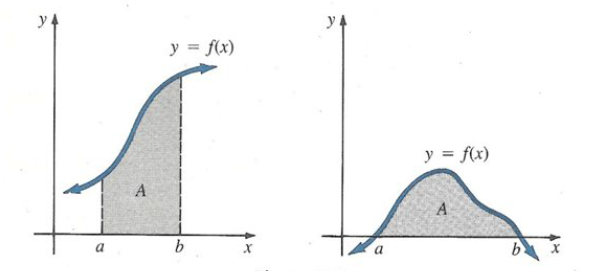
\includegraphics[width=0.5\textwidth]{area.png}\\[1cm]
  \end{center}
\section{Riemann Sums}
Thinking integral as area, you can approximate the value of an integral by approximating the area. A \textbf{Riemann Sum} is a sum of areas of rectangles. To estimate $\displaystyle \int _a^b f(x)\, dx$, where $a<b$. 
\begin{center}
 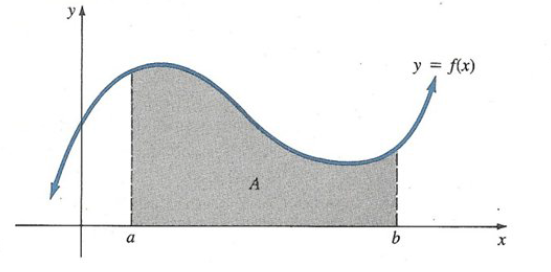
\includegraphics[width=0.5\textwidth]{area1.png}\\[1cm]
  \end{center}
\noindent First, divide the interval $[a,b]$ into $n$ subintervals, using $x_0, x_1, x_2, \dots , x_n$ as endpoints for the subintervals, 
\begin{equation*}
a=x_0<x_1<\cdots <x_{n-1}<x_n=b.
\end{equation*}
The subintervals are then 
\begin{equation*}
[x_0, x_1], [x_1, x_2], \cdots , [x_{n-1}, x_n].
\end{equation*} 
For simplicity, let the subintervals have the same length, $\Delta x =\dfrac{b-a}{n}$. You then have $x_i=a+i\Delta x$. Choose a point $c$ in each subinterval and construct a rectangle above the subinterval with height $f(c)$. For simplicity, above the $i$th subinterval $[x_{i-1}, x_i]$ make the height of the rectangle $f(x_i)$. The sum of the area of the rectangles is an approximation to $\displaystyle \int _a^b f(x)\, dx$. The $i$th rectangle has width $\Delta x$ and height $f(x_i)$, hence the area $A_i=f(x_i)\Delta x$. Thus :
\begin{eqnarray*}
\int _a^b f(x)\, dx &\approx &  A_1 +A_2 +\cdots +A_n \\
&=& f(x_1)\Delta x +f(x_2)\Delta x +\cdots +f(x_n)\Delta x \\
&=& \sum _{i=1}^n f(x_i)\Delta x.
\end{eqnarray*}
This is the Riemann Sum for the integral $\displaystyle \int _a^b f(x)\, dx$. In general, if you increase $n$, you will improve your approximation.

\noindent \textbf{Example:} Find the area of the region bounded by the graphs of $f(x)=2x, \, x=0, \, x=1$ and the $x$-axis by calculating the limit of the Riemann Sums.

\noindent \textbf{Solution:} First divide the interval $[0,1]$ into $n$ subintervals of equal length, 
\begin{equation*}
\Delta x =\dfrac{b-a}{n}=\dfrac{1-0}{n}=\dfrac{1}{n}.
\end{equation*}
Therefore, 
\begin{equation*}
x_i=a+i\Delta x =0+i\cdot \dfrac{1}{n}=\dfrac{i}{n}.
\end{equation*}
The $n$th Riemann Sum is 
\begin{eqnarray*}
\sum _{i=1}^n f(x_i)\Delta x &=& \sum _{i=1}^n f\left(\dfrac{i}{n}\right) \Delta x \\
&=& \sum _{i=1}^n 2\left(\dfrac{i}{n}\right) \Delta x =\sum _{i=1}^n 2\left(\dfrac{i}{n}\right)\left(\dfrac{1}{n}\right)\\
&=&\sum _{i=1}^n \dfrac{2}{n^2}i
\end{eqnarray*}
Inside the summation, $\dfrac{2}{n^2}$ does not involve $i$, and so you can pull it outside the summation.
\begin{eqnarray*}
\sum _{i=1}^n \dfrac{2}{n^2}i &=& \dfrac{2}{n^2}\sum _{i=1}^n i \\
&=& \dfrac{2}{n^2}\left[\dfrac{n(n+1)}{2}\right] =\dfrac{2n^2+2n}{2n^2}\\
&=& 1+\dfrac{1}{n}.
\end{eqnarray*}
Finally, you can find the limit of the Riemann Sums :
\begin{equation*}
\lim _{n\rightarrow \infty} \sum _{i=1}^n f(x_i)\Delta x =\lim _{n\rightarrow \infty} \left(1+\dfrac{1}{n}\right)=1.
\end{equation*}


\noindent \textbf{Example:} Find the area of the region bounded by the graphs of $f(x)=(x-1)^2+2, \, x=-1, \, x=2$ and the $x$-axis by finding the limit of the Riemann Sums.

\noindent \textbf{Solution:} Divide $[-1,2]$ as follows $\Delta x =\dfrac{2-(-1)}{n}=\dfrac{3}{n}$, then $x_i=a+i\Delta x =-1+\dfrac{3i}{n}$. Then,  the $n$th Riemann Sum is \\
\begin{eqnarray*}
\sum _{i=1}^n f(x_i)\Delta x &=&\sum _{i=1}^n f\left(-1+\dfrac{3i}{n}\right) \cdot \dfrac{3}{n} \\
&=& \sum _{i=1}^n \left[\left(-1+\dfrac{3i}{n}-1\right)^2+2\right]\cdot \dfrac{3}{n} \\
&=& \sum _{i=1}^n  \left[\left(\dfrac{3i}{n}-2\right)^2+2\right]\cdot \dfrac{3}{n} \\
&=& \sum _{i=1}^n \left[\dfrac{9i^2}{n^2}-\dfrac{12i}{n}+4+2\right] \cdot \dfrac{3}{n} 
\end{eqnarray*}
\begin{eqnarray*}
&=& \sum _{i=1}^n \left[\dfrac{27}{n^3}i^2-\dfrac{36}{n^2}i+\dfrac{18}{n}\right]\\
&=& \dfrac{27}{n^3}\sum _{i=1}^n i^2-\dfrac{36}{n^2}\sum _{i=1}^n i+\dfrac{18}{n}\sum _{i=1}^n 1\\
&=& \dfrac{27}{n^3} \left[\dfrac{n(n+1)(2n+1)}{6}\right]-\dfrac{36}{n^2}\left[\dfrac{n(n+1)}{2}\right]+\dfrac{18}{n}(n)\\
&=&\dfrac{9(n+1)(2n+1)}{2n^2}-\dfrac{18(n+1)}{n}+18.
\end{eqnarray*}
The area is the limit of the Riemann Sum 
\begin{equation*}
\lim _{n\rightarrow \infty} \sum _{i=1}^n f(x_i)\Delta x =\lim _{n\rightarrow \infty} \left[ \dfrac{9(n+1)(2n+1)}{2n^2}-\dfrac{18(n+1)}{n}+18\right] =9-18-18 =9.
\end{equation*}

\noindent \textbf{You Try It:} Find the area of the function $f(x)=x$ on $[0,1]$ by finding the limit of the Riemann Sums.
\subsection{The Definite Integral}
The geometric problems that motivated the development of the integral calculus (determination of
lengths, areas, and volumes) arose in the ancient civilizations of Northern Africa. Where solutions were
found, they related to concrete problems such as the measurement of a quantity of grain. Greek
philosophers took a more abstract approach. In fact, Eudoxus (around 400 B.C.) and Archimedes
(250 B.C.) formulated ideas of integration as we know it today.
Integral calculus developed independently, and without an obvious connection to differential
calculus. The calculus became a ‘‘whole’’ in the last part of the seventeenth century when Isaac Barrow,
Isaac Newton, and Gottfried Wilhelm Leibniz (with help from others) discovered that the integral of a
function could be found by asking what was differentiated to obtain that function.

\begin{definition}
Let $f$ be a function defined on a closed interval $[a,b]$. Then the \textbf{definite integral} of $f$ from $a$ to $b$, denoted by $\displaystyle \int _{a}^b f(x)\, dx$, is defined to be 
\begin{equation*}
\int _{a}^b f(x)\, dx =\lim _{n\rightarrow \infty}\sum _{i=1}^n f(x_i)\Delta x.
\end{equation*}
\end{definition}
\noindent The numbers $a$ and $b$ are called the \textbf{lower} and \textbf{upper limits of integration}, respectively. If the limit exists, the function $f$ is said to be \textbf{integrable} on the interval. 
\subsection{Properties of the Definite Integral}
The following two definitions prove to be useful when working with definite integrals.
\begin{theorem}
If $f(a)$ exists, then 
\begin{equation*}
\int _a^a f(x)dx=0.
\end{equation*}
\end{theorem}
\begin{theorem}
If $f$ is integrable on $[a,b]$, then 
\begin{equation*}
\int _b^a f(x)dx=-\int _a^b f(x)dx.
\end{equation*}
\end{theorem}
\noindent \textbf{Example:} By definition 
\begin{equation*}
\int _1^1 (x^3+3x)dx=0.
\end{equation*}
\begin{theorem}
Let $f$ and $g$ be integrable functions on $[a,b]$. Then, 
\begin{itemize}
\item[(i)] $\displaystyle \int _{a}^b kf(x)\, dx=k\int _{a}^b f(x)\, dx$ where $k$ is any constant.
\item[(ii)] $\displaystyle \int _{a}^b [ f(x) \pm g(x)]\, dx=\int _{a}^b f(x)\, dx \pm \int _{a}^b g(x)\, dx$.
\item[(iii)] $\displaystyle \int _{a}^b f(x)\, dx=\int _{a}^c f(x)\, dx +\int _{c}^b f(x)\, dx$, where $c$ is any number in $[a,b]$.
\end{itemize}
\end{theorem}
\noindent The independent variable $x$ in a definite integral is called a \textbf{dummy variable} of integration. The value of the integral does not depend on the symbol used. In other words, 
\begin{equation*}
\int _{a}^b f(x)\, dx =\int _{a}^b f(r)\, dr =\int _{a}^b f(s)\, ds =\int _{a}^b f(t)\, dt
\end{equation*}
and so on.
\begin{theorem}
For any constant $k$, 
\begin{equation*}
\int _{a}^b k\, dx =k\int _{a}^b dx=k(b-a).
\end{equation*}
\end{theorem}
\begin{theorem}
Let $f$ be integrable on $[a,b]$ and $f(x)\geq 0$ for all $x$ in $[a,b]$, then 
\begin{equation*}
\int _{a}^b f(x)\, dx\geq 0.
\end{equation*}
\end{theorem}
\section{The Fundamental Theorem of Calculus}
In this theorem we shall see that the concept of an anti-derivative of a continuous function provides the bridge between the differential calculus and the integral calculus. 
\begin{theorem}
Let $f$ be continuous on $[a,b]$ and let $F$ be any function for which $F'(x)=f(x)$. Then 
\begin{equation*}
\int _{a}^b f(x)\, dx=F(b)-F(a).
\end{equation*}
\end{theorem}
\noindent The difference is usually written 
\begin{equation*}
F(x)\biggl|_{a}^b,
\end{equation*} 
that is, 
\begin{equation*}
\underbrace{\int _a^b f(x)\, dx}_{\hbox{definite integral}} =\underbrace{\int f(x)\, dx\biggl|_a^b}_{\hbox{indefinite integral}} =F(x)\biggl|_{a}^b.
\end{equation*}

\noindent \textbf{Example:} Evaluate $\displaystyle \int _{1}^3 x\, dx$.

\noindent \textbf{Solution:} An anti-derivative  of $f(x)=x$ is $F(x)=\dfrac{x^2}{2}$. Consequently, 
\begin{equation*}
\int _{1}^3 x\, dx =\dfrac{x^2}{2}\biggl|_{1}^3=\dfrac{9}{2}-\dfrac{1}{2}=4.
\end{equation*}
\section{Techniques of Integration}
\subsection{Integration by Parts}
Useful for integrands involving products of algebraic and exponential or logarithmic functions, such as $\displaystyle \int x^2e^x\, dx$ and $\displaystyle \int x\ln x\, dx$. This is the inverse operation of differentiating a product. If $u$ and $v$ are functions of $x$, then 
\begin{equation*}
\dfrac{d}{dx}(uv)=u\dfrac{dv}{dx}+v\dfrac{du}{dx}.
\end{equation*}
Integrate both sides, if $\dfrac{du}{dx}$ and $\dfrac{dv}{dx}$ are continuous, then 
\begin{eqnarray*}
uv &=& \int u\dfrac{dv}{dx}\, dx +\int v\dfrac{du}{dx}\, dx \\
\int u \dfrac{dv}{dx}\, dx &=& uv -\int v\dfrac{du}{dx}\, dx \\
\int u \, dv &=& uv -\int v\, du.
\end{eqnarray*}

\noindent \textbf{Example:} Evaluate $\displaystyle \int xe^x \, dx$.

\noindent \textbf{Solution:} Let $u=x, \, du=dx$ and $dv=e^x\, dx\Rightarrow v=\displaystyle \int dv=\int e^x\, dx=e^x$. Then, 
\begin{equation*}
\int xe^x \, dx=xe^x-e^x+C.
\end{equation*}

\noindent \textbf{Example:} Evaluate $\displaystyle \int x^2 \ln x\, dx$.

\noindent \textbf{Solution:} $x^2$ is more easily integrated than $\ln x$. So choose $dv=x^2\, dx$. Then, 
\begin{equation*}
dv=x^2\, dx \Rightarrow v=\int dv =\int x^2 \, dx =\dfrac{x^3}{3}.
\end{equation*}
and $u=\ln x \Rightarrow du=\dfrac{1}{x}\, dx$. Therefore, 
\begin{eqnarray*}
\int x^2 \ln x\, dx &=& \dfrac{x^3}{3}\ln x -\int \left(\dfrac{x^3}{3}\right)\left(\dfrac{1}{x}\right)\, dx\\
&=& \dfrac{x^3}{3}\ln x -\dfrac{1}{3}\int x^2\, dx \\
&=&  \dfrac{x^3}{3}\ln x -\dfrac{x^3}{9}+C.
\end{eqnarray*}

\noindent \textbf{Example:} Evaluate $\displaystyle \int \ln x \, dx$.

\noindent \textbf{Solution:} Choose $dv=dx \Rightarrow v=\displaystyle \int dv=\int dx=x$ and $u=\ln x\Rightarrow du=\dfrac{1}{x}\, dx$, therefore
\begin{eqnarray*}
\int \ln x\, dx &=& x\ln x -\int x\cdot \dfrac{1}{x}\, dx \\
&=& x\ln x -\int dx\\
&=&x\ln x -x+C.
\end{eqnarray*}

\noindent \textbf{You Try It:} Evaluate $\displaystyle \int x\tan ^{-1} x \, dx$.

\section{Using Integration by Parts Repeatedly}
\textbf{Example:} Evaluate $\displaystyle \int x^2e^x\, dx$.

\noindent \textbf{Solution:} Notice that the derivative of $x^2$ becomes simpler, whereas the derivative of $e^x$ does not. So you should let $u=x^2$ and $dv=e^x\, dx$. So 
\begin{eqnarray*}
dv=e^x\, dx  &\Rightarrow & v=\int dv=\int e^x\, dx =e^x\\
u=x^2 &\Rightarrow & du=2x\, dx.
\end{eqnarray*}
Integrating by parts one time we get, 
\begin{equation*}
\int x^2e^x\, dx =x^2e^x-\int 2xe^x\, dx.
\end{equation*}
Apply integration by parts a second time, where 
\begin{eqnarray*}
dv=e^x \, dx &\Rightarrow & v=\int dv =\int e^x \, dx =e^x\\
u=2x &\Rightarrow & du=2\, dx.
\end{eqnarray*}
Then, 
\begin{eqnarray*}
\int x^2e^x\, dx &=& x^2e^x-\int 2xe^x\, dx\\
&=& x^2e^x-\left(2xe^x-\int 2e^x\, dx\right)\\
&=& x^2e^x-2xe^x+2e^x+C\\
&=& e^x(x^2-2x+2)+C.
\end{eqnarray*}
\section{Evaluating a Definite Integral}
\textbf{Example:} Evaluate $\displaystyle \int _{1}^e \ln x \, dx$.

\noindent \textbf{Solution:} 
\begin{eqnarray*}
 \int _{1}^e \ln x \, dx &=& (x\ln x -x)\biggl |_{1}^e \\
 &=& (e\ln e -e)-(1\cdot \ln 1 -1)\\
 &=& (e-e)-(0-1)\\
 &=& 1.
\end{eqnarray*}
\section{Reduction Formulas}
These are formulas in which a given integral is expressed in terms of similar integrals of simpler form. 

\noindent \textbf{Example:} Let $n$ be a positive integer. Use integration  by parts to derive the reduction formula 
\begin{equation*}
\int x^n e^x\, dx =x^ne^x-n\int x^{n-1}e^x\, dx +C.
\end{equation*}

\noindent \textbf{Solution:} Let $u=x^n, \, dv=e^x\, dx$. Then $du=nx^{n-1}$, $v=\displaystyle \int dv=\int e^x \, dx=e^x$. So 
\begin{eqnarray*}
\int x^ne^x\, dx &=&x^ne^x-\int e^x(nx^{n-1})\, dx \\
&=& x^ne^x-n\int x^{n-1}e^x\, dx +C.
\end{eqnarray*} 
To illustrate the use of the reduction formula we calculate $\displaystyle \int x^ne^x\, dx$ for $n=1,2$.
\begin{eqnarray*}
n=1 &:& \int xe^x\, dx =xe^x-\int e^x\, dx=xe^x-e^x+C.\\
n=2 &:& \int x^2e^x\, dx =x^2e^x-2\int xe^x\, dx =x^2e^x-2xe^x+2e^x+C.
\end{eqnarray*}


\noindent \textbf{Example:} Evaluate $\displaystyle \int \sin ^n x \, dx$.

\noindent \textbf{Solution:} Rewrite as $\displaystyle \int \sin ^n x\, dx =\int \sin ^{n-1}x \sin x\, dx$. \\Then $u=\sin ^{n-1}x \Rightarrow du=(n-1)\sin ^{n-2}x \cos x\, dx$ and $dv=\sin x \Rightarrow \\ v=\displaystyle \int dv=\int \sin x \, dx =-\cos x$. Then , 
\begin{eqnarray*}
\int \sin ^n x \, dx &=&-\sin ^{n-1}x \cos x +(n-1)\int \sin ^{n-2}x \cos x \cos x \, dx\\
&=&-\sin ^{n-1}x \cos x +(n-1)\int \sin ^{n-2}x \cos ^2 x\, dx\\
&=&-\sin ^{n-1}x \cos x+(n-1)\int \sin ^{n-2}x (1-\sin ^2 x)\, dx\\
&=&-\sin ^{n-1}x \cos x+(n-1)\left[\int \sin ^{n-2}x \, dx -\sin ^n x \, dx\right]\\
\int \sin ^n x \, dx +(n-1)\int \sin ^n x \, dx &=&-\sin ^{n-1}x \cos x +(n-1)\int \sin ^{n-2}x \, dx\\
n\int \sin ^n x \, dx &=&-\sin ^{n-1}x \cos x +(n-1)\int \sin ^{n-2}x \, dx \\
\int \sin ^n x \, dx &=&- \dfrac{\sin ^{n-1}x\cos x}{n} +\dfrac{n-1}{n}\int \sin ^{n-2}x\, dx.
\end{eqnarray*}
\section{Partial Fractions}
This technique involves the decomposition of a rational function into the sum of two or more simpler rational functions. We will consider rational functions (quotients of polynomials) in which the numerator has a lower degree than the denominator. If this condition is not meet, we first carry out long division process, dividing the denominator into the  numerator, until we reduce the problem to an equivalent one involving a fraction in which the numerator has a lower degree than the denominator. 

\noindent \textbf{Example:} $\dfrac{x+7}{x^2-x-6}=\dfrac{2}{x-3}-\dfrac{1}{x+2}$, then 
\begin{eqnarray*}
\int \dfrac{x+7}{x^2-x-6}\, dx &=&\int \left(\dfrac{2}{x-3}-\dfrac{1}{x+2}\right)\, dx \\
&=& 2\int \dfrac{1}{x-3}\, dx -\int \dfrac{1}{x+2}\, dx\\
&=& 2\ln |x-3|-\ln |x+2| +C.
\end{eqnarray*}

\noindent \textbf{You Try It:} Evaluate $\displaystyle \int \dfrac{2x+1}{(x-1)(x+3)}\, dx$.
\subsection{Integrating with Repeated Factors}
 \textbf{Example:} Find $\displaystyle \int \dfrac{5x^2+20x+6}{x^3+2x^2+x}\, dx$.
 
 \noindent \textbf{Solution:} Factorise the denominator as $x(x+1)^2$. Then write the partial decomposition as 
 \begin{equation*}
 \dfrac{5x^2+20x+6}{x(x+1)^2}=\dfrac{A}{x}+\dfrac{B}{x+1} +\dfrac{C}{(x+1)^2}.
 \end{equation*}
 Substituting we get, $A=6, \, B=-1, \, C=9$, then 
 \begin{eqnarray*}
 \int \dfrac{5x^2+20x+6}{x^3+2x^2+x}\, dx &=& \int \dfrac{6}{x}\, dx -\int \dfrac{1}{x+1}\, dx +\int \dfrac{9}{(x+1)^2}\, dx\\
 &=& 6\ln |x|-\ln |x+1|+\dfrac{9(x+1)^{-1}}{-1} +C\\
 &=& \ln \left|\dfrac{x^6}{x+1}\right|-\dfrac{9}{x+1}+C.
 \end{eqnarray*}
 
 \noindent \textbf{You Try It:} Evaluate $\displaystyle \int \dfrac{6x-1}{x^3(2x-1)}\, dx$.
 \subsection{Integrating an Improper Rational Function}
 \textbf{Example:} Find $\displaystyle \int \dfrac{x^5+x-1}{x^4-x^3}\, dx$.
 
 \noindent \textbf{Solution:} This rational is improper, its numerator has a degree greater than that of its denominator. Carrying out long division, we have
 \begin{equation*}
\dfrac{x^5+x-1}{x^4-x^3} =x+1 +\dfrac{x^3+x-1}{x^4-x^3}.
 \end{equation*}
 Now, applying partial fraction decomposition produces
 \begin{equation*}
 \dfrac{x^3+x-1}{x^3(x-1)} =\dfrac{A}{x}+\dfrac{B}{x^2}+\dfrac{C}{x^3}+\dfrac{D}{x-1}.
 \end{equation*}
 We see that $A=0, \, B=0, \, C=1$ and $D=1$. So now we can integrate, 
 \begin{eqnarray*}
 \int \dfrac{x^5+x-1}{x^4-x^3}\, dx &=& \int \left(x+1+\dfrac{x^3+x-1}{x^4-x^3}\right)\, dx\\
 &=& \int \left(x+1+\dfrac{1}{x^3}+\dfrac{1}{x-1}\right)\, dx\\
 &=& \dfrac{x^2}{2}+x-\dfrac{1}{2x^2}+\ln |x-1|+C.
 \end{eqnarray*}
 
 \noindent \textbf{You Try It:} Evaluate $\displaystyle \int \dfrac{x^3-2x}{x^2+3x+2}\, dx$.
 \subsection{Quadratic Factors}
 \textbf{Example:} Find $\displaystyle \int \dfrac{dx}{x^2-4x+5}$.
 
 \noindent \textbf{Solution:} Here we cannot find real factors, but we can complete the square, 
 \begin{equation*}
 x^2-4x+5=(x-2)^2+1, 
 \end{equation*}
 therefore 
 \begin{equation*}
 \int \dfrac{dx}{x^2-4x+5} =\int \dfrac{dx}{(x-2)^2+1}=\tan ^{-1} (x-2) +C.
 \end{equation*}
 
 
 \noindent \textbf{Example:} Find $\displaystyle \int \dfrac{(x+3)dx}{x^2-4x+5}$.
 
 \noindent \textbf{Solution:} Completing the square, $\dfrac{x+3}{x^2-4x+5}=\dfrac{x+3}{(x-2)^2+1}$. Now since $x+3=x-2+5$, we have 
 \begin{eqnarray*}
 \int \dfrac{(x+3)dx}{x^2-4x+5} &=&\int \dfrac{(x-2+5)\, dx}{(x-2)^2+1}\\
 &=& \int \dfrac{(x-2)\, dx}{(x-2)^2+1} +\int \dfrac{5\, dx}{(x-2)^2+1}\\
 &=& \dfrac{1}{2}\ln ((x-2)^2+1)+5\tan ^{-1} (x-2)+C.
 \end{eqnarray*}
 
 \noindent \textbf{Example:} Find $\displaystyle \int \dfrac{(x+1)\, dx}{x(x^2+1)}$.
 
 \noindent \textbf{Solution:} Decompose into partial fractions, 
 \begin{equation*}
 \dfrac{x+1}{x(x^2+1)}=\dfrac{A}{x}+\dfrac{B+Cx}{x^2+1}.
 \end{equation*}
 Then $A=1, \, B=1, \, C=-1$, and our integral is 
 \begin{eqnarray*}
 \int \dfrac{(x+1)\, dx}{x(x^2+1)} &=& \int \dfrac{1}{x}\, dx +\int \dfrac{dx}{x^2+1}-\int \dfrac{x\, dx}{x^2+1}\\
 &=& \ln |x| +\tan ^{-1} x-\dfrac{1}{2}\ln (x^2+1)+C.
 \end{eqnarray*}
 
 \noindent \textbf{You Try It:} Evaluate $\displaystyle \int \dfrac{4x}{(x^2+1)(x^2+2x+3)}\, dx$.
 \section{Integration of Rational Functions of Sine and Cosine}
 Integrals of rational expressions that involve $\sin x$ and $\cos x$ can be reduced to integrals of quotients of polynomials by means of the substitution 
 \begin{equation*}
 t=\tan \left(\dfrac{x}{2}\right).
 \end{equation*}
 It then follows that $\cos x=\dfrac{1-t^2}{1+t^2}, \, \sin x =\dfrac{2t}{1+t^2}$ and $\dfrac{dx}{dt}=\dfrac{2}{1+t^2}$.
 
 \noindent \textbf{Example:} Evaluate $\displaystyle \int \dfrac{dx}{2+2\sin x+\cos x}$.
 
 \noindent \textbf{Solution:} We see that 
 \begin{equation*}
 \int \dfrac{dx}{2+2\sin x+\cos x} =\int \dfrac{2\, dt}{t^2+4t+3}.
\end{equation*}  
Since $t^2+4t+3=(t+1)(t+3)$, we use partial fractions, 
\begin{eqnarray*}
 \int \dfrac{dx}{2+2\sin x+\cos x} &=&\int \left(\dfrac{1}{t+1}-\dfrac{1}{t+3}\right)\, dt\\
 &=& \ln |t+1|-\ln |t+3|+C\\
 &=&\ln \left|\dfrac{t+1}{t+3}\right| +C\\
 &=&\ln \left|\dfrac{1+\tan \frac{x}{2}}{3+\tan \frac{x}{2}}\right| +C.
\end{eqnarray*}

\noindent \textbf{Example:} Evaluate $\displaystyle \int \dfrac{dx}{5+3\cos x}$.

\noindent \textbf{Solution:} The integral becomes 
\begin{eqnarray*}
\int \dfrac{dx}{5+3\cos x} &=& \int \dfrac{\dfrac{2dt}{1+t^2}}{5+3\left(\dfrac{1-t^2}{1+t^2}\right)}\\
&=& \int \dfrac{\dfrac{2dt}{1+t^2}}{\dfrac{5(1+t^2)+3(1-t^2)}{1+t^2}} = \int \dfrac{2dt}{8+2t^2}\\
&=& \int \dfrac{dt}{t^2+4} = \dfrac{1}{2}\tan ^{-1} \left(\frac{t}{2}\right) +C\\
&=& \dfrac{1}{2}\tan ^{-1} \left(\dfrac{1}{2}\tan \frac{x}{2}\right)+C.
\end{eqnarray*}

\noindent \textbf{You Try It:} Evaluate $\displaystyle \int \dfrac{dx}{5+4\cos x}$.

\section{Integration of Powers of Trigonometric Functions}
With the aid of trigonometric identities, it is possible to evaluate integrals of the type
\begin{equation*}
\int \sin ^m x \cos ^n x \, dx.
\end{equation*}
We distinguish two cases.\\

\noindent \textbf{Case 1: $m$ or $n$ is an odd positive integer.} Let us first assume that $m$ is an odd positive integer. By writing 
\begin{equation*}
\sin ^m x =\sin ^{m-1}x \sin x, 
\end{equation*} 
where $m-1$ is even, and using $\sin ^2 x =1-\cos ^2 x$, the integrand can be expressed as a \textit{sum} of powers of $\cos x$ times $\sin x$.

\noindent \textbf{Example:} Evaluate $\displaystyle \int \sin ^3 x\, dx$.

\noindent \textbf{Solution:} 
\begin{eqnarray*}
\int \sin ^3 x\, dx &=&\int \sin ^2 x\sin x \, dx\\
&=& \int (1-\cos ^2 x)\sin x \, dx \\
&=&\int \sin x\, dx +\int \cos ^2 x (-\sin x)\, dx\\
&=& -\cos x +\dfrac{1}{3}\cos ^3 x +C.
\end{eqnarray*}


\noindent \textbf{Example:} Evaluate $\displaystyle \int \sin ^5 x \cos ^2x\, dx$.

\noindent \textbf{Solution:}
\begin{eqnarray*}
\int \sin ^5 x \cos ^2 x\, dx &=& \int \cos ^2 x\sin ^4 x \sin x\, dx\\
&=& \int \cos ^2 x (\sin ^2 x)^2 \sin x \, dx\\
&=& \int \cos ^2 x (1-\cos ^2 x)^2 \sin x \, dx\\
&=& \int \cos ^2 x (1-2\cos ^2 x+\cos ^4 x)\sin x \, dx\\
&=& -\int \cos ^2 x (-\sin x)\, dx +2\int \cos ^4 x (-\sin x)\, dx -\int \cos ^6 x(-\sin x)\, dx \\
&=&-\dfrac{1}{3}\cos ^3 x +\dfrac{2}{5}\cos ^5 x-\dfrac{1}{7}\cos ^7 x +C.
\end{eqnarray*}
If $n$ is an odd positive integer, the procedure for evaluation is the same except that we seek an integrand that is the sum of powers of $\sin x$ times $\cos x$.

\noindent \textbf{Example:} Evaluate $\displaystyle \int \sin ^4 x \cos ^3 x\, dx$.

\noindent \textbf{Solution:} 
\begin{eqnarray*}
\int \sin ^4 x \cos ^3 x\, dx &=& \int \sin ^4 x \cos ^2 x \cos x\, dx\\
&=& \int \sin ^4 x (1-\sin ^2 x)\cos x\, dx\\
&=& \int \sin ^4 x (\cos x)\, dx -\sin ^6 x (\cos x)\, dx\\
&=&\dfrac{1}{5}\sin ^5 x -\dfrac{1}{7}\sin ^7 x +C.
\end{eqnarray*}
 \noindent \textbf{You Try It:} Evaluate $\displaystyle \int \sin ^2 x \cos ^3 x \, dx$.
 
 \noindent \textbf{Case II: $m$ and $n$ are both even non-negative integers.} When both $m$ and $n$ are even non-negative integers, the evaluation of the integral relies heavily on the identities, 
 \begin{equation*}
 \sin x \cos x =\dfrac{1}{2}\sin 2x, \quad \sin ^2 x =\dfrac{1-\cos 2x}{2}, \quad \cos ^2 x =\dfrac{1+\cos 2x}{2}.
\end{equation*}

\noindent \textbf{Example:} Evaluate $\displaystyle \int \cos ^4 x \, dx$.

\noindent \textbf{Solution:} 
\begin{eqnarray*}
 \int \cos ^4 x \, dx &=& \int (\cos ^2 x)^2 \,dx\\
 &=& \int \left(\dfrac{1+\cos 2x}{2}\right)^2 \, dx\\
 &=& \dfrac{1}{4}\int (1+2\cos 2x +\cos ^2 2x)\, dx\\
 &=&\dfrac{1}{4}\int \left(1+2\cos 2x+\dfrac{1+\cos 4x}{2}\right)\, dx\\
 &=& \dfrac{1}{4} \int \left(\dfrac{3}{2}+2\cos 2x+\dfrac{1}{2}\cos 4x\right)\, dx\\
 &=& \dfrac{3}{8}x+\dfrac{1}{4}\sin 2x +\dfrac{1}{32}\sin 4x +C.
\end{eqnarray*}
\textbf{You Try It:} Evaluate $\displaystyle \int \sin ^2 x \cos ^2 x\, dx$.  

\noindent Instead of $\sin ^8 x \cos ^6 x$, suppose you have $\sin 8x\cos 6x$.

\noindent \textbf{Example:} Find $\displaystyle \int _0^{2\pi}\sin 8x \cos 6x \, dx$.

\noindent More generally, find $\displaystyle \int _0^{2\pi} \sin px \cos qx\, dx$. Use the identity 
\begin{equation*}
\sin px \cos qx =\dfrac{1}{2}\sin (p+q)x +\dfrac{1}{2}\sin (p-q)x.
\end{equation*}
Thus $\sin 8x\cos 6x=\dfrac{1}{2}\sin 14x +\dfrac{1}{2}\sin 2x$. Separated like this, sine are easy to integrate, 
\begin{equation*}
\int _{0}^{2\pi}\sin 8x \cos 6x \, dx =\left(-\dfrac{1}{2}\dfrac{\cos 14x}{14}-\dfrac{\cos 2x}{4}\right)\biggl| _{0}^{2\pi}=0.
\end{equation*}
With two sines or two cosines, the addition formula, derive these formulas, 
\begin{eqnarray*}
\sin px \cos qx  &=& -\dfrac{1}{2}\cos (p+q)x+\dfrac{1}{2}\cos (p-q)x.\\
\cos px \cos qx &=& \dfrac{1}{2}\cos (p+q)x +\dfrac{1}{2}\cos (p-q)x.
\end{eqnarray*}

\noindent \textbf{You Try It:} Evaluate $\displaystyle \int \sin 2x \sin 4x\, dx$.
\section{Tutorial Questions}
\begin{enumerate}
\item Find the area of the region bounded by the graphs of $f(x)=2(x+2)^3, x=-2, x=0$ and the $x$-axis by calculating the Riemann sums.
\item Show that the function $f(x)=x$ on $[0,1]$ is Riemann integrable by calculating the Riemann sums.
\item Evaluate the following.\\
(i)\, $\displaystyle \int (x+2)\sin (x^2+4x-6)dx$ \quad (ii)\, $\displaystyle \int x^2e^{\sin x^3}\cos x^3 dx$ \quad (iii)\, $\displaystyle \int \dfrac{\tan ^{-1} x}{1+x^2}dx$ \\ (iv)\, $\displaystyle \int \dfrac{dx}{x(\ln x)^4}$ \quad (v)\, $\displaystyle \int x^2\sqrt{2x^3-4}dx$ \quad (vi)\, $\displaystyle \int \dfrac{3x}{\sqrt[3]{2x^2+3}}dx$ \quad (vii)\, $\displaystyle \int \dfrac{x\sin ^{-1}x^2}{\sqrt{1-x^4}}dx$.
\item Integrate (i)\, $\dfrac{1}{(x^2+1)(x+1)}$ \quad (ii)\, $\dfrac{x+5}{(2x-1)(x+3)}$ \quad (iii)\, $\dfrac{2x-5}{(x^2+4)(x+6)}$.
\item Evaluate each of the following integrals by using an appropriate substitution.\\
(i)\, $\displaystyle \int \dfrac{x^5 dx}{\sqrt{x^3+1}}$ \quad (ii)\, $\displaystyle \int x^7\sqrt{x^4+1}dx$ \quad (iii)\, $\displaystyle \int \sqrt{\dfrac{1+x}{1-x}}dx$ \quad (iv)\, $\displaystyle \int \dfrac{x}{2+\sqrt{x+1}}dx$\\ (v)\, $\displaystyle \int  \dfrac{x^{\frac{2}{3}}}{1+x^{\frac{1}{2}}}dx$ \quad (vi)\, $\displaystyle \int \dfrac{1}{x^{\frac{1}{2}}+x^{\frac{1}{4}}}dx$ \quad (vii)\, $\displaystyle \int \dfrac{\sqrt[3]{x}}{1+\sqrt{x}}dx$.
\item Evaluate each of the following integrals.\\
(i)\, $\displaystyle \int \sin ^3 x dx$ \quad (ii)\, $\displaystyle \int \sin x \cos x dx$ \quad (iii)\, $\displaystyle \int \sin ^3 x \cos ^3 x dx$ \quad (iv)\, $\displaystyle \int \sin 6x \cos 3x dx$ \quad (v)\, $\displaystyle \int \cos x \cos 4x dx$ \quad (vi)\, $\displaystyle \int \sin 2x\sin 4x\, dx$ \quad (vii)\, $\displaystyle \int _0^{\frac{\pi}{2}}\sin \frac{3}{2}x \cos \frac{1}{2}x\, dx$.
\item Use a suitable substitution to evaluate the following integrals.\\
(i)\, $\displaystyle \int \sec \theta d\theta$ \quad (ii)\, $\displaystyle \int \dfrac{d\theta}{1+\sin \theta}$ \quad (iii)\, $\displaystyle \dfrac{\sin \theta}{2+\sin \theta}d\theta$ \quad (iv)\, $\displaystyle \int \dfrac{d\theta}{a+b\cos \theta}$ if $a>b>0$.
\item Evaluate each of the following integrals.\\
(i)\, $\displaystyle \int xe^{3x}dx$ \quad (ii)\, $\displaystyle \int e^x\sin x dx$ \quad (iii)\, $\displaystyle \int \tan ^{-1} x dx$ \quad (iv)\, $\displaystyle \int e^{ax}\cos px dx $\quad (v)\, $\displaystyle \int x^3\cos x dx$.
\item 
\begin{itemize}
\item[(a)] Show that $\displaystyle \int x^m \ln x dx=x^{m+1}\left(\dfrac{\ln x}{m+1}-\dfrac{1}{(m+1)^2} \right), \, m \neq -1$.
\item[(b)] Show that $\displaystyle \int \sin ^n x dx=\dfrac{-\sin ^{n-1}x \cos x}{n}+\dfrac{n-1}{n}\int \sin ^{n-2}x dx, \, n\neq 0$.
\item[(c)] Show that $\displaystyle \int x^n e^{ax}dx=\dfrac{x^ne^{ax}}{a}-\dfrac{n}{a}\int x^{n-1}e^{ax}dx, \, n>0$.
\item[(d)] Show that $\displaystyle \int \sin ^m x \cos ^n x dx=-\dfrac{\sin ^{m-1}x \cos ^{n+1}x}{m+n}+\dfrac{m-1}{m+n}\int \sin ^{m-2} x \cos ^n xdx$ and so find $\displaystyle \int \sin ^6x \cos ^5 x dx$.
\item[(e)] Let $I_n=\displaystyle \int \sec ^n x dx, \, n=2,3,\dots$. Show that $I_n=\dfrac{\sec ^{n-2}x \tan x}{n-1}+\dfrac{n-2}{n-1}I_{n-2}$.
\item[(f)] Let $I_n=\displaystyle \int (\ln x)^n dx, n=1,2,\dots$. Show that $I_n=x(\ln x)-nI_{n-1}$.
\item[(g)] Let $\displaystyle I_n=\int x^ne^xdx, n=1,2,3,\dots$. Show that $I_n=x^ne^x-I_{n-1}$. Find $\displaystyle \int x^3e^xdx$.
\item[(h)] Let $I_n=\displaystyle \int (1+ax^2)^n dx$. Show that $(2n+1)I_n=2nI_{n-1}+x(1+ax^2)^n$.
\item[(i)] Let $\displaystyle \int _{0}^a (x^2+a^2)^{\frac{n}{2}}dx$. Show that $(n+1)I_n=2^{\frac{n}{2}}a^{n+1}+na^2I_{n-2}$.
\end{itemize}
\end{enumerate}
\end{document}